%%%%%%%%%%%%%%%%%%%%%%%%%%%%%%%%%%%%%%%%%
% Beamer Presentation
% LaTeX Template
% Version 1.0 (10/11/12)
%
% This template has been downloaded from:
% http://www.LaTeXTemplates.com
%
% License:
% CC BY-NC-SA 3.0 (http://creativecommons.org/licenses/by-nc-sa/3.0/)
%
%%%%%%%%%%%%%%%%%%%%%%%%%%%%%%%%%%%%%%%%%

%----------------------------------------------------------------------------------------
%	PACKAGES AND THEMES
%----------------------------------------------------------------------------------------

\documentclass[10]{article}
\pagestyle{plain}

\usepackage{graphicx} % Allows including images
\usepackage{booktabs} % Allows the use of \toprule, \midrule and \bottomrule in tables
\usepackage{blkarray} % Allows the use of labelled matrices
\usepackage{amsmath,amsfonts,amssymb}
\usepackage{mathtools}
%\usepackage[plain]{algorithm}
\usepackage{algorithm}
\usepackage[noend]{algpseudocode}

\usepackage[utf8]{inputenc}
\usepackage[english]{babel}
\usepackage{amsthm}

\usepackage{subcaption}

%\usepackage{setspace}
%\onehalfspacing
%\doublespacing
\usepackage{longtable}
%\usepackage[demo]{graphicx}
%\usepackage{tikz,pgfplots} 

% set margins
\usepackage[margin=1.0in]{geometry}

\newtheorem{theorem}{Theorem}[section]
%\newtheorem{corollary}{Corollary}[theorem]
\newtheorem{corollary}[theorem]{Corollary}
\newtheorem{lemma}[theorem]{Lemma}
\newtheorem{definition}{Definition}[section]
%\newtheorem{definition}[theorem]{Definition}


\graphicspath{{figs/}}

\usepackage{color}
%\usepackage{hyperref}       
%\usepackage{varioref}       
%\usepackage{cleveref}
\usepackage[colorlinks=true, allcolors=blue]{hyperref}


% declaration of the new block
\algblock{ParFor}{EndParFor}
% customising the new block
\algnewcommand\algorithmicparfor{\textbf{parallel for}}
\algnewcommand\algorithmicpardo{\textbf{do}}
\algnewcommand\algorithmicendparfor{\textbf{end parfor}}
\algrenewtext{ParFor}[1]{\algorithmicparfor\ #1\ \algorithmicpardo}
\algrenewtext{EndParFor}{\algorithmicendparfor}

% supprese EndParFor
\makeatletter
\ifthenelse{\equal{\ALG@noend}{t}}%
  {\algtext*{EndParFor}}
  {}%
\makeatother


\newcommand{\push}[1]{\text{push} \left ( #1 \right )}
\newcommand{\pop}{\text{pop}()}

\DeclareMathOperator*{\argmax}{arg\,max}
\DeclareMathOperator*{\argmin}{arg\,min}

\newcommand{\algoname}[1]{\textnormal{\textsc{#1}}}

\newcommand{\E}{\mathbb{E}}
\newcommand{\Var}{\mathrm{Var}}
\newcommand{\Cov}{\mathrm{Cov}}
\newcommand{\Bias}{\mathrm{Bias}}
\newcommand{\med}{\mathrm{median}}
\newcommand{\mean}{\mathrm{mean}}
%\newcommand{\argmax}{\mathrm{argmax}}
%\newcommand{\argmin}{\mathrm{argmin}}
\newcommand{\poly}{\mathrm{poly}}
\newcommand{\polylog}{\, \mathrm{polylog} \,}
\newcommand{\el}{\mathrm{else}}
\newcommand{\diag}{\mathrm{diag}}
\newcommand{\rank}{\mathrm{rank}}
\newcommand{\nnz}{\mathrm{nnz}}

%----------------------------------------------------------------------------------------
%	TITLE PAGE
%----------------------------------------------------------------------------------------

\title{Degree{S}ketch: Distributed Cardinality Sketches on Graphs with Applications}
\author{Benjamin W. Priest}
\date{\today} % Date, can be changed to a custom date

\begin{document}

\maketitle

\begin{abstract}
The identification of important vertices or edges is a ubiquitous problem in the analysis of graphs.
There are many application-dependent measures of importance, such as centrality indices (e.g. degree centrality, closeness centrality, betweenness centrality, and eigencentrality) and local triangle counts, among others.
Traditional computational models assume that the entire input fits into working memory, which is impractical for very large graphs.
The distributed memory model and streaming model are popular solutions to this problem of scale.
In the distributed memory model a collection of processors partition the graph and must optimize communication in addition to execution time.
The data stream model assumes only sequential access to the input, which is handled in small chunks.
Data stream algorithms use sublinear memory and a small number of passes and seek to optimize update time, query time, and post processing time.  

In this dissertation, we consider the application of distributed data stream algorithms to the sublinear approximation of several centrality indices, local triangle counts, and the simulation of random walks. 
We pay special attention to the recovery of \emph{heavy hitters} - the largest elements relative to the given index.

The first part of this dissertation focuses on serial graph stream algorithms.
We present new algorithms providing streaming approximations of degree centrality and a semi-streaming constant-pass approximation of closeness centrality.
We achieve our results by way of counting sketches and sampling sketches.

The second part of this dissertation considers vertex-centric distributed graph stream algorithms.
We develop hybrid pseudo-asynchronous communication protocols tailored to managing communication on distributed graph algorithms with asymmetric computational loads.
We use this protocol as a framework to develop distributed streaming algorithms utilizing cardinality sketches.
We present new algorithms for estimating local neighborhood sizes, as well as vertex- and edge-local triangle counts, with special attention paid to heavy hitter recovery.
We also utilize reservoir sampling and $\ell_p$ sampling sketches to optimize the semi-streaming simulation of many random walks in parallel in distributed memory.
We use these algorithms to approximate  $K$-path centrality as a proxy for recovery the top-$k$ betweenness centrality elements.
\end{abstract}

%\keywords{graph processing, evolving graphs, centrality, data stream model, sketching, pass-constrained algorithms}


%----------------------------------------------------------------------------------------
%----------------------------------------------------------------------------------------
\section{Introduction} \label{chap:intro}
%----------------------------------------------------------------------------------------
%----------------------------------------------------------------------------------------
\pagenumbering{arabic}



Many modern computing problems focus on complex relationship networks arising from real-world data. 
Many of these complex systems such as the Internet, communication networks, logistics and transportation systems, biological systems, epidemiological models, and social relationship networks map naturally onto graphs \cite{wasserman1994social}.
%These networks, sometimes labeled ``social networks'' due to their roots in human behavior, often exhibit similar structure and submit to similar analyses. 
A natural question that arises in the study of such networks is how to go about identifying ``important'' vertices and edges.
How one might interpret importance within a graph is contingent upon its domain.
Accordingly, investigators have devised a large number of importance measures that account for different structural properties. 
These measures implicitly define an ordering on graphs, and typically only the top elements vis-\'a-vis the ordering are of analytic interest.

However, most traditional RAM algorithms scale poorly to large datasets. 
This means that very large graphs tend to confound standard algorithms for computing various important orderings. 
Newer computational models such as the data stream model and the distributed memory model were introduced to address these scalability concerns.
The data steam model assumes only sequential access to the data, and permits a sublinear amount of additional working memory.
The time to update, query, and post process this data structure, as well as the number of passes and amount of additional memory are the important resources to optimize in the data stream model.
The data stream model is a popular computational model for handling scalability in sequential algorithms.
The distributed memory model partitions the data input across several processors, which may need to subsequently communicate with each other.
The amount of communication is an important optimization resource.
In practical terms, minimizing the amount of time processors spend waiting on their communication partners is also important.

Although both models have been applied to very large graphs independently, there is relatively little literature focusing on the union of the two models of computation. 
In this work we devise distributed data stream algorithms to approximate orderings of vertices and edges of large graphs. 
We focus in particular on recovering the heavy hitters of these orderings.
We consider the sublinear approximation of classic centrality scores, as well as local and global triangle counts.
We also describe space-efficient methods for sampling random walks and subtrees in scale-free vertex-centric distributed graphs, and their application to estimating some centrality indices.

%----------------------------------------------------------------------------------------
\section{Data Stream Models} \label{intro:sec:data_stream}
%----------------------------------------------------------------------------------------


\textbf{The data stream model}:
A stream $\sigma = \langle a_1, a_2, \dots, a_m \rangle$ is a sequence of elements in the universe $\mathcal{U}$, $|\mathcal{U}|=n$.
We assume throughout that that the hardware has working memory storage capabilities $o( \min \{m, n\})$.
We will use the notation $[p] = \{ 1, 2, \dots, p-1, p \}$ for $p \in \mathbb{Z}_{> 0}$ throughout for compactness. 
For $t \in [m]$, we will sometimes refer to the state of $\sigma$ after reading $t$ updates as $\sigma(t)$.
%Thus, clearly, storing $\sigma$ in working memory is not an option.
A streaming algorithm $\mathcal{A}$ accumulates a data structure $\mathcal{S}$ while reading over $\sigma$. 
We will sometimes use the notation $\mathcal{D}(\sigma)$ to indicate the data structure state after $\mathcal{A}$ has accumulated $\sigma$. 
Authors generally assume $|\mathcal{D}| = \widetilde{O}(1) = O(\log m + \log n)$, where here the tilde suppresses logarithmic factors.
We will also adopt the convention that, except where noted otherwise, we present space complexities in terms of machine words rather than bits.
Except where noted otherwise, we will assume the base 2 logarithm in our presentation.

\noindent
\textbf{The semi-streaming model}:
Unfortunately, logarithmic memory constraints are not always possible.
In particular, it is known that many fundamental properties of complex structured data such matrices and graphs require memory linear in some dimension of the data \cite{mahoney2011randomized, mcgregor2009graph}.
In such cases, the logarithmic requirements of streaming algorithms are sometimes relaxed to $O(n \polylog n)$ memory, where $\polylog n = \Theta(\log^c n)$ for some constant $c$. 
In the case of matrices, here $n$ refers to one of the matrix's dimensions, whereas for graphs $n$ refers to the number of vertices.
This is usually known as the \emph{semi-streaming model}, although some authors also use the term to refer to $O(n^{1+\gamma})$ for small $\gamma$ \cite{feigenbaum2005graph, muthukrishnan2005data}.

\noindent
\textbf{The frequency vector and dynamic streams}:
A stream $\sigma$ is often thought of as updates to a hypothetical frequency vector $\mathbf{f}(\sigma)$, which holds a counter for each element in $\mathcal{U}$.
We will drop the parameterization of $\mathbf{f}$ where it is clear.
We will sometimes parameterize $\mathbf{f}(t)$ to refer to $\mathbf{f}$ after reading $t \in [m]$ updates from $\sigma$.
$\mathcal{D}$ can be thought of as a lossy compression of $\mathbf{f}$ that approximately preserves some statistic thereof.
%
%\noindent
%\textbf{Dynamic streams}:
%If $\mathbf{f}$ is subject to change, then we call $\sigma$ a \emph{turnstile} or \emph{dynamic} stream.
The stream $\sigma$'s elements are of the form $(i, c)$, where $i$ is an index of $\mathbf{f}$ (an element of $\mathcal{U}$), $c \in [-L, \dots, L]$ for some integer $L$, and $(i,c)$ indicates that $\mathbf{f}_i \gets \mathbf{f}_i + c$.
Such a stream $\sigma$ is called a \emph{turnstile} or sometimes \emph{dynamic} stream. 
In the \emph{cash register} model only positive updates are permitted, whereas in the \emph{strict} turnstile model all elements of $\mathbf{f}$ are guaranteed to retain nonnegativity.

\noindent
\textbf{Data sketching}:
Let $\circ$ be the concatenation operator on streams.
For $\mathcal{A}$ a streaming algorithm, we call its data structure $\mathcal{S}$ a \emph{sketch transform} if there is an operator $\oplus$ such that, for any streams $\sigma_1$ and $\sigma_2$, 
%
\begin{equation} \label{eq:merge}
\mathcal{S}(\sigma_1) \oplus \mathcal{S}(\sigma_2) = \mathcal{S}(\sigma_1 \circ \sigma_2).
\end{equation}
%
$\mathcal{S}$ is usually determined by sampling hash functions from a suitable hash family. 
We will call the distribution over such samples $\Pi$ a \emph{sketch distribution}.
The accumulated object $\mathcal{S}(\sigma)$ is a sketch data structure.
We will sometimes abuse terms and refer to $\Pi$, $\mathcal{S}$, and $\mathcal{S}(\sigma)$ as \emph{sketches}.
The space of all possible sketch data structures given a sketch transform $\mathcal{S}$ is the sketch space $\mathbb{S}_\mathcal{S}$.
$(\mathbb{S}_\mathcal{S}, \oplus)$ forms a commutative monoid, where the operator identity is the result of applying $\mathbb{S}$ to an empty stream.

\noindent
\textbf{Linear sketching}:
A sketch distribution $\Pi$ is a \emph{linear sketch} distribution if $\mathcal{S} \sim \Pi$ is a linear function of frequency vectors $\mathbf{f}(\cdot)$ of fixed dimension.
%Typically $\mathcal{S}$ is drawn from a distribution $\Pi$ over such transforms.
%We will abuse terminology by referring to sketch distributions, sketch transforms, and sketch data structures as sketches where it is clear which is referenced.
%In particular, any turnstile streaming algorithm uses a linear sketch as a data structure \cite{li2014turnstile}.
%
For streams $\sigma_1$ and $\sigma_2$ with frequency vectors $\mathbf{f}_1$ and $\mathbf{f}_2$, scalars $a$ and $b$, and linear sketch transform $\mathcal{S}$, 
%
\begin{equation} \label{eq:linearity}
a\mathcal{S}(\mathbf{f}_1) + b\mathcal{S}(\mathbf{f}_2) = \mathcal{S}(a\mathbf{f}_1 + b\mathbf{f}_2).
\end{equation}
%
The sketch space and the $+$ operator form a commutative group, where the operator identity is the sketch transform applied to a zero vector.

\noindent
\textbf{The graph stream model}:
In this model, the stream $\sigma$ consists of $m$ edge insertions on $n$ vertices. 
This is sometimes termed the \emph{insert only} model in the literature.
The \emph{dynamic graph stream model} also allows edge deletions.
If the graph is weighted, the stream updates the weight of the corresponding edge, possibly bringing it into existence or, in the case of dynamic streams, deleting it.


\noindent
\textbf{DegreeSketch and local triangle count heavy hitters}:
Counting global and local triangles is a canonical problem in both the random access and data stream models. 
In the data stream model it is known that $\Omega(n^2)$ space is required to even decide whether a graph has any triangles \cite{bar2002reductions}.
Vertex-local triangle counts are similarly fraught in the data stream model, as they require $\Omega(n)$ space to even write them down. 
Recent advances in the graph stream literature achieve low variance via clever sampling from edge streams \cite{becchetti2008efficient, lim2015mascot, stefani2017triest}, and have been distributed to achieve better variance \cite{shin2018tri, shin2018dislr}.

We examine a different line of analysis altogether: utilizing \emph{cardinality sketches} to estimate local triangle counts via a sublinearization of the set intersection method.
We discuss trade-offs between different estimators of the intersection of cardinality sketches, as well as different cardinality sketches themselves.
We develop \algoname{DegreeSketch}, a distributed sketch data structure composed of cardinality sketches that can answer point queries about unions and intersections of vertex neighborhoods in a manner reminiscent of \algoname{CountSketch}.

We implement \algoname{DegreeSketch} using the famous \algoname{HyperLogLog} sketch \cite{flajolet2007hyperloglog}. 
We explore various algorithmic optimizations to \algoname{HyperLogLog}, including improved estimators \cite{heule2013hyperloglog, qin2016loglog, lang2017back, ertl2017new}, sparse register implementation \cite{heule2013hyperloglog}, and compressed registers \cite{xiao2017better}.
We introduce novel improvements to the compressed register implementation described in \cite{xiao2017better}, affording lossless merging of compressed sketches.
We also discuss the tradeoffs of using different cardinality sketches in implementations, such as \algoname{MinCount} \cite{giroire2009order}.

We demonstrate DegreeSketch as a tool for estimating local neighborhood sizes, as well as the edge- and vertex-local triangle count heavy hitters of large graphs. 
%
\begin{enumerate}
	\item \textbf{Local neighborhood size and neighborhood function}. We estimate the local neighborhood sizes and global neighborhood function of a graph using linear time and $O(n (\varepsilon^{-2} \log\log n + \log n))$ worst-case distributed memory
	\item \textbf{Edge-local triangle count heavy hitters}. We estimate the edge-local triangle count heavy hitters of a graph using the same asymptotic time and memory requirements.
	\item \textbf{Vertex-local triangle counts}. We estimate the vertex-local triangle counts (or, alternately, the heavy hitters) of a graph using the same asymptotic time and memory requirements.
%	linear time and \\$O(n (\varepsilon^{-2} \log\log n + \log n))$ worst-case distributed memory
\end{enumerate}
%
We analyze the performance of these algorithms on numerous large graphs, and discuss many practical optimizations to the underlying algorithms. 
We also discuss the limitations of the approach relating to high variance on small intersections and intersections of sets of differing sizes.


%------------------------------------------------
%------------------------------------------------
\section{Background and Notation} \label{chap:background}
%------------------------------------------------
%------------------------------------------------

This chapter introduces the basic concepts and notation that we will use throughout this document.
We will lay out the basic graph, probability, and linear algebraic definitions and notation conventions that will be referenced later
We also describe centrality indices as a class of functions on graphs.
Finally, we describe $k$-universal hash families, an important concept for many sketches, as well as some approximation definitions.
%Section \ref{sec:approx} introduces the major approximation paradigms we will consider throughout this document. 
%Section \ref{sec:turnstile} describes the turnstile model of computation and formally defines important streaming data primitives. 
%Section \ref{sec:sketch} discusses sketching in detail, and introduces the most important classes of sketches that we will use throughout this document. 
%It also delivers a brief overview of existing semi-streaming graph algorithms. 



%----------------------------------------------------------------------------------------
%----------------------------------------------------------------------------------------
\section{Graph Definitions and Notation} \label{background:sec:graphdef}
%----------------------------------------------------------------------------------------
%----------------------------------------------------------------------------------------

Throughout this document we will consider the graph $\mathcal{G} = (\mathcal{V}, \mathcal{E}, \mathbf{w})$.
We assume that $\mathcal{G}$ has no self loops, and that where $|\mathcal{V}| = n$ and $|\mathcal{E}| = m$.
For convenience of reference and indexing, we will often assume that $\mathcal{V} = [n]$ and $E = [m]$. 
%For convenience, we will usually assume that $\mathcal{V} = \{ 0, 1, \dots, n -1 \}$ and use elements of $V$ as subscripts.
We denote an edge connecting $x, y \in \mathcal{V}$ as $xy \in \mathcal{E}$. 
In general we will assume that $\mathcal{G}$ is an  undirected graph, except where noted otherwise. 
When we want to specify a direction on an edge, we will use the tuple notation $(x, y)$ for $x, y \in \mathcal{V}$.
If $\mathcal{G}$ is a weighted graph, then $\mathbf{w} \in \mathbb{R}^{{n \choose 2}}$ is the vector of edge weights. 
For $x, y \in \mathcal{V}$, $\mathbf{w}_{xy} \in \mathbb{R}_{\geq 0}$ is the weight associated with the edge $xy$ if $xy \in \mathcal{E}$, and is zero otherwise.
If $\mathcal{G}$ is unweighted, then $\mathbf{w}_e = 1$ for every $e \in \mathcal{E}$. 

Let $A \in \mathbb{R}^{n\times n}$ be the \emph{adjacency matrix} of $\mathcal{G}$, where $A_{x,y} = \mathbf{w}_{xy}$.
We will adopt the convention that, if $\mathcal{G}$ is unweighted, then the columns of $A$ correspond to the out edges whereas the rows of $A$ correspond to the in edges. 
Hence, $A_{:,x}$ is the out adjacency vector of vertex $x$, and $A_{x,:}$ is its in adjacency vector.

For $\mathcal{G}$ an unweighted graph, let $D \in \mathbb{R}^{n\times n}$ be a diagonal matrix, where $D_{x,x}$ is the \emph{degree} or \emph{valency} of vertex $x \in \mathcal{V}$, which can be computed as the row sum of the $x$th row of $A$. 
We define $L = D - A$ as the \emph{Laplace Matrix} or \emph{Laplacian} of $\mathcal{G}$.

Consider the signed vertex-edge incidence matrix, $B \in \mathbb{R}^{{n \choose 2} \times n}$, given by
%
\begin{equation} \label{eq:veim}
B_{xy,z} = 
\begin{cases}
1 & \textnormal{if $xy \in \mathcal{E}$ and $x=z$} \\
-1 & \textnormal{if $xy \in \mathcal{E}$ and $y=z$} \\
0 & \textnormal{else}.
\end{cases}
\end{equation}
%
Here we let $x$, $y$, and $z$ range over $\mathcal{V}$. 
Let $W \in \mathbb{R}^{n \times n}$ be a diagonal matrix such that $W_{x,y} = \sqrt{w_{xy}}$.
Then if $G$ is undirected, we can alternatively write the Laplacian as 
%
\begin{equation} \label{eq:laplacian}
L = BWW^TB^T.
\end{equation}
%
If $\mathcal{G}$ is unweighted, then we can simply write $L = BB^T$. 

%We define some more basic definitions below. 
A \emph{path} in $\mathcal{G}$ is a series of edges $(x_1 x_2, x_2 x_3, \dots, x_{\ell -1} x_\ell)$ where the tail of each edge is the head of the following edge in the path. 
The length, alternatively weight, of a path is the sum of the weights of all of its edges.
If G is unweighted, this is simply the number of edges in the path.
We can equivalently identify the path with the series of vertices $(x_1, x_2, \dots, x_\ell)$, where an edge links each $x_i, x_{i+1}$ pair.
For vertices $x,y \in \mathcal{V}$, the \emph{distance} $d_\mathcal{G}(x,y)$ between $x$ and $y$ in $\mathcal{G}$ is the length of the shortest path that begins at $x$ and ends with $y$. 
There may be more than one such path. 
If there is no path connecting $x$ to $y$ in $\mathcal{G}$, then we say that $d_\mathcal{G}(x,y) = \infty$. 
If the graph is clear from context, we may omit the subscripts and write $d(x,y)$.
We call a path \emph{simple} if it visits every vertex no more than once. 


%----------------------------------------------------------------------------------------
\section{Centrality Indices} \label{sec:centrality}
%----------------------------------------------------------------------------------------

A centrality index is any map $\mathcal{C}$ that assigns to every $x \in \mathcal{V}$ a nonnegative score.
The particulars of $\mathcal{C}$ are usually assumed to be conditioned only on the structure of $\mathcal{G}$.
Consequently, we can identify the centrality index on $\mathcal{G}$ as a function $\mathcal{C}_\mathcal{G} : \mathcal{V} \rightarrow \mathbb{R}_{\geq 0}$.
For $x \in \mathcal{V}$, we will call $\mathcal{C}_\mathcal{G}(x)$ the centrality score of $x$ in $\mathcal{G}$. 
Typically, for $x,y \in \mathcal{V}$, $\mathcal{C}_\mathcal{G}(x) > \mathcal{C}_\mathcal{G}(y)$ implies that $x$ is more important than $y$ in $\mathcal{G}$ with respect to the property that $\mathcal{C}$ measures. 
We will generally drop the subscript from $\mathcal{C}$ when it is clear from context. 
It is important to note that if $\mathcal{G}$ changes, so may the mapping $\mathcal{C}$. 
At times, we will write $\mathcal{C}(\mathcal{G})$ or $\mathcal{C}(\mathcal{V})$ to denote the set of all centrality scores of the vertices in $\mathcal{G}$. 

Researchers have considered more exotic centrality indices that rely on metadata, such as vertex and edge colorings \cite{kang2016diffusion}.
Such notions of centrality are most likely out of scope for the research proposed by this document. 
%Thinking of a centrality index as a function of $G$ will be important in subsequent sections. 


%----------------------------------------------------------------------------------------
%----------------------------------------------------------------------------------------
\section{Vector and Matrix definitions and notation} \label{sec:matdef}
%----------------------------------------------------------------------------------------
%----------------------------------------------------------------------------------------



For a vector $v \in \mathbb{R}^n$, we denote the $\ell_p$ norm as follows:
%
\begin{equation} \label{eq:pnorm}
\|v\|_p = \left( \sum\limits_{i=1}^n |v_i|^p \right )^{1/p}.
\end{equation}
%
As $p \rightarrow 0$, this quantity converges to the special case of the $\ell_0$ norm:
%
\begin{equation} \label{eq:0norm}
\|v\|_0 = \sum_{i=1}^n v_i^0 =  | \{ i \in [n] \mid v_i \neq 0 \} |.
\end{equation}
%
Here we define $0^0 = 0$. 
Throughout this document we will mostly be concerned with the $\ell_0$ and $\ell_1$ norms of matrix rows and columns. 
The $p$-th frequency moment $F_p$ of a vector $v$ is related to its $\ell_p$ norm in the following way:
%
\begin{equation} \label{eq:Fp}
F_p(v) = \|v\|_p^p = \sum\limits_{i=1}^n v_i^p.
\end{equation}
%
%Given a vector $v \in \mathbb{R}^n$, we use the notation $v_{-i}$ to denote the vector whose elements are all the same as $v$ aside from the $i$th element, which is zero.
%
%Much of the literature in the sketching and streaming communities has to do with estimating $\ell_p$ norms or $F_p$ moments of streaming vectors. 




We will also sometimes be interested in matrix norms. 
For $i \in [n]$ and $j \in [m]$, we will write the $i,j$th element of $M$ as $M_{i,j}$. 
We will also write the $i$th row and $j$th column of $M$ as $M_{i,:}$ and $M_{:,j}$, respectively. 
For a matrix $M \in \mathbb{R}^{n \times m}$, we define the Fr\"obenius norm as follows:
%
\begin{equation} \label{eq:fnorm}
\|M\|_F = \left( \sum\limits_{i=1}^n \sum\limits_{j=1}^m M_{i,j}^2 \right )^{1/2}.
\end{equation}
%

Given $A \in \mathbb{R}^{n\times d}$, let $A = U\Sigma V^T$ be its singular value decomposition (SVD), where $\Sigma \in \mathbb{R}^{n \times n}$ is a diagonal matrix and $U$ and $V$ are orthonormal.
Set $A_k = U_k \Sigma_k V^T_k$, where $U_k$ and $V_k$ are the leading $k$ columns of $U$ and $V$, respectively, and $\Sigma_k \in \mathbb{R}^{k \times k}$ is a diagonal matrix whose entries are the first $k$ entries of $\Sigma$. 
$A_k$ is known to solve the optimization problem
%
\begin{equation*}
\min\limits_{\widetilde{A} \in \mathbb{R}^{n \times d}: \rank(\widetilde{A}) \leq k} \|A-\widetilde{A}\|_F.
\end{equation*}
%
That is, $A_k$ is the rank-$k$ matrix which has the smallest Fr\"obenius residual with $A$.
This is also true of the spectral norm. 
We will sometimes denote the rank-$k$ truncated SVD of a product of matrices $A_1\cdots A_n$ as $[A_1\cdots A_n]_k$.
We use the notation $A^+ = V \Sigma^{-1} U^T$ to denote the Moore-Penrose Pseudoinverse of $A$. 








%----------------------------------------------------------------------------------------
%----------------------------------------------------------------------------------------
\section{\algoname{DegreeSketch} with Applications to Neighborhood Approximation and Local Triangle Count Heavy Hitter Estimation}
 \label{chap:DS}
%----------------------------------------------------------------------------------------
%----------------------------------------------------------------------------------------


In this chapter we present \algoname{DegreeSketch}, a semi-streaming distributed sketch datastructure and demonstrate its utility for estimating local triangle count heavy hitters.
\algoname{DegreeSketch} consists of vertex-centric cardinality sketches distributed across a set of processors. 
While other semi-streaming approaches to estimating local triangle counts depend on sampling, \algoname{DegreeSketch} is a persistent queryable data structure.
We discuss the advantages and limitations of this approach, and present empirical results.

%----------------------------------------------------------------------------------------
\section{Introduction and Related Work}
 \label{DS:sec:intro}
%----------------------------------------------------------------------------------------

Counting the number of triangles in simple graphs is a canonical problem in both the RAM and streaming models.
A ``triangle'' is a trio of co-adjacent vertices, and is the smallest nontrivial community structure.
Consequently, triangles and triangle counting arise often in applications.
Both the global count of triangles and the vertex-local counts, i.e. the number of triangles incident upon each vertex, are key to network analysis and graph theory topics such as cohesiveness \cite{lim2015mascot}, global and local clustering coefficients \cite{tsourakakis2008fast}, and trusses \cite{cohen2008trusses}.
These counts are also directly useful in many applications, such as spam detection \cite{becchetti2010efficient},  community discovery \cite{wang2010triangulation, berry2011tolerating}, and protein interaction analysis \cite{milo2002network}.

Although not traditionally considered a centrality index, one can think of the number of triangles incident upon a vertex as a generalization of its degree centrality. 
To wit, we define the \emph{triangle count centrality} of a vertex $x \in \mathcal{V}$ as
%
\begin{equation}
	\mathcal{C}^{\algoname{Tri}}(x) = |\{yz \in \mathcal{E} \mid xy, zx \in \mathcal{E} \wedge |\{x, y, z\}| = 3\}|.
\end{equation}
%
We can consider the triangle count centrality of edges as well, defined similarly as
%
\begin{equation}
	\mathcal{C}^{\algoname{Tri}}(xy) = |\{z \in \mathcal{V} \setminus \{x,y\} \mid yz, zx \in \mathcal{E}\}|.
\end{equation}
%
We will also refer to the total number of triangles in a graph 
%
\begin{equation}
	\mathcal{T}_\mathcal{G} = |\{ \{xy, yz, zx\} \in \mathcal{E} \mid |\{x, y, z\}| = 3 \} |.
\end{equation}
%

Although many exact algorithms have been proposed for the triangle counting problem \cite{tsourakakis2008fast, becchetti2010efficient, chu2011triangle, suri2011counting, wolf2017fast}, their time complexity is superlinear in the number of edges, $O(m^{
\frac{3}{2}})$.
Consequently, these analyses are expensive on very large graphs, particularly if they are dense.
While there is a rich literature centered on the exact global and local triangle counting problem, we will not exhaustively recall it in this document.

In order to avoid the dreaded superlinear scaling of exact algorithms, many researchers have turned to approximation.
Several streaming local triangle counting algorithms have been proposed in recent years.
These serial streaming algorithms  maintain a limited number of sampled edges from an edge stream.
Streaming global triangle estimation algorithms have arisen that sample edges with equal probability \cite{tsourakakis2009doulion}, sample edges with probability relative to counted adjacent sampled edges and incident triangles \cite{ahmed2017sampling}, and sample edges along with paths of length two \cite{jha2013space}. 
The first proposed semi-streaming local triangle estimation algorithm relies upon min-wise independent permutations accumulated over a logarthmic number of passes \cite{becchetti2008efficient}. 
More recently, true single-pass algorithms have arisen such as \algoname{Mascot} \cite{lim2015mascot}, which maintains local estimates that are updated whether an observed edge is sampled or not.
Similarly, \algoname{Tri\'est} \cite{stefani2017triest} utilizes reservoir sampling, possibly disposing of sampled edges when a new edge is observed if system memory is saturated.
This affords robustness to dynamic streams, as well as reducing variance.
None of these algorithms perform edge-local triangle counting.

While many distributed global and vertex-local triangle counting algorithms have been proposed, the overwhelming majority store the graph in distributed memory and return exact solutions using \algoname{MapReduce} \cite{suri2011counting} or distributed memory \cite{arifuzzaman2013patric, pearce2017triangle}.
Recently, the study of distributed streaming vertex-local triangle counting was intiated in earnest with the presentation of \algoname{Try-Fly} \cite{shin2018tri}, which maintains parallel instantiations of \algoname{Tri\'est$_{\algoname{Impr}}$}.
A controller node feeds partitions of the graph stream to each of these instances in order to boost estimation accuracy and speed.
\algoname{DiSLR} \cite{shin2018dislr} improves upon \algoname{Try-Fly} by introducing limited redundancy into the graph stream partitions.
Although \algoname{Try-Fly} and \algoname{DiSLR} are the most similar examples in the literature to our approach, we use distinct methods.

Our approach is fundamentally different, depending upon sketching rather than sampling as its core primitive. 
While the sampling approaches produce estimates, we produce a leave-behind queryable data structure similar in interface to \algoname{CountMinSketch}.

%These algorithms depends upon sampling edges from an edge stream in order to assemble a sparse graph, whose triangles are then used to estimate the true local triangle counts.
%The most successful recent algorithm \algoname{Tri\'est} utilizes reservoir sampling to afford dynamic graph streams as well as to affect a reduction in variance.
%Very recent distributed streaming algorithms boost the performance of underlying sampling algorithms such as \algoname{Tri\'est} by utilizing parallel machines operating on partitions of the input graph \cite{shin2018tri, shin2018dislr}.

%----------------------------------------------------------------------------------------
\section{\algoname{DegreeSketch} via Distributed Cardinality Sketches}
 \label{DS:sec:DS}
%----------------------------------------------------------------------------------------

We take a different approach to estimating local triangle counts, relying upon sketches instead of sampling.
We introduce \algoname{DegreeSketch}, a cardinality sketch-based distributed data structure trained on graph streams.
We will first describe \algoname{DegreeSketch} at a high level, describe algorithms that utilize it in Sections~\ref{DS:sec:neighborhoods}, ~\ref{DS:sec:edge_triangles}, and ~\ref{DS:sec:vertex_triangles} and then discuss implementation details using the \algoname{HyperLogLog} cardinality sketch in Section~\ref{DS:sec:HLL}.

\algoname{DegreeSketch} maintains a data structure $\mathcal{D}$ that can be queried for an estimate of a vertex's degree, similar in interface to the celebrated \algoname{CountSketch} \cite{charikar2002finding} and \algoname{CountMinSketch} \cite{cormode2005improved}.
This data structure is organized not unlike the sampling sketch approach to graph sparsification discussed in Section~\ref{sec:spanner}, with sketches summarizing the local information for each $x \in \mathcal{V}$.
For each $x \in \mathcal{V}$ we maintain a cardinality sketch $\mathcal{D}[x]$, which affords the approximation of $\mathbf{d}_x$, the degree of $x$. 
%We obtain estimates of local triangle counts by comparing the sketches of adjacent vertices.

It is known that any data structure that provides relative error guarantees for the cardinality of a multiset with $n$ unique elements requires $O(n)$ space \cite{alon1999space}.
Consequently, investigators have developed many so-called \emph{cardinality sketches} that provide such relative error guarantees while admitting a small probability of failure, such as PCSA \cite{flajolet1985probabilistic}, MinCount \cite{bar2002counting},  LogLog \cite{durand2003loglog}, Multiresolution Bitmap \cite{estan2003bitmap}, HyperLogLog \cite{flajolet2007hyperloglog}, and the space-optimal solution of \cite{kane2010optimal}.
While all these cardinality sketches have a natural union operation that allows one to combine the sketches of two multisets into a sketch of their union, most have no closed intersection operation.

For the purposes of discussion, we will abstract the particulars of cardinality sketches until Section~\ref{DS:sec:HLL}.
We assume that the sketches provide a $\varepsilon$-approximation of the number of unique items in a stream using $\Omega(\varepsilon^{-2})$ space.
We assume that the sketches support an \algoname{Insert} operation to add elements, a \algoname{Merge} operation to combine sketches, an \algoname{Estimate} operation to estimate cardinalities, and an \algoname{EstimateIntersection} operation to estimate intersection cardinalities.
For reasons that will be described in Section~\ref{DS:sec:HLL:intersection}, we do not assume that the \algoname{EstimateIntersection} procedure has the same error and variance properties as the guarantees for \algoname{Estimate}.

We will describe the accumulation of a \algoname{DegreeSketch} instance on a universe of processors $\mathcal{P}$. 
We assume that the undirected graph $\mathcal{G} = (\mathcal{V}, \mathcal{E})$ is given by a stream $\boldsymbol{\sigma}$.
$\boldsymbol{\sigma}$ is further partitioned by some unknown means into $|\mathcal{P}|$ substreams.
We assume that each processor $P \in \mathcal{P}$ has send and receive buffers $\mathcal{S}[P]$ and $\mathcal{R}[P]$, respectively.
We will make no assumptions in the following algorithms how processors handle switching context between processing and sending and receiving communication. 
In our implementations we use the software package \algoname{YGM}, developed as a part of this thesis and described in Chapter~\ref{chap:async}.
\algoname{YGM} manages the send and receive buffers, as well as switching contexts, in a manner that is opaque to the client algoirthm.
We further assume that there is some partitioning of vertices to processors $f : \mathcal{V} \rightarrow \mathcal{P}$. 
We will occasionally abuse notation and use $f(P)$ to describe the set of vertices that map to $P \in \mathcal{P}$.
We make no assumptions about the particulars of $f$, noting that vertex partitionings are a subject of intense academic scrutiny as discussed in Section~\ref{async:sec:intro:partitioning}.
In effect, our algorithms are designed to work alongside any decent partitioning mechanism. 

Algorithm~\ref{alg:ds:accumulation} describes the distributed accumulation of a \algoname{DegreeSketch} instance.
In a distributed pass over the partitioned stream, processors use the partition function $f$ to send edges to the cognizant processors for each endpoint. 
These processors each maintain cardinality sketches for their assigned vertices.
When $P \in \mathcal{P}$ receives an edge $xy \in \mathcal{E}$ where $f(x) = P$, it performs $\algoname{Insert}(\mathcal{D}[x], y)$.
Once all processors are done reading and communicating, $\mathcal{D}$ is accumulated.

\begin{algorithm}[htbp] 
\caption{\algoname{DegreeSketch} Accumulation}\label{alg:ds:accumulation}
\begin{flushleft}
        \textbf{Input:} 		$\boldsymbol{\sigma}$ - edge stream divided into $|\mathcal{P}|$ substreams\\
        	\hspace{3.2em}	$\mathcal{P}$ - universe of processors	 \\
%        	\hspace{2.65em}	$\mathcal{D}$ - distributed dictionary mapping $\mathcal{V}$ to cardinality sketches	 \\
        	\hspace{3.2em}	$\mathcal{S}$ - distributed dictionary mapping $\mathcal{P}$ to send queues	 \\
        	\hspace{3.2em}	$\mathcal{R}$ - distributed dictionary mapping $\mathcal{P}$ to receive queues	 \\
        	\hspace{3.2em}	$f$ - function mapping $\mathcal{V} \rightarrow \mathcal{P}$	 \\
        \textbf{Output:} $\mathcal{D}$ - accumulated DegreeSketch
\end{flushleft}
\begin{flushleft}
\begin{algorithmic}[1]
	\Statex \textbf{Send Context} for $P \in \mathcal{P}$:
		\While{$\mathcal{S}[P]$ is not empty}
  			\State $(W, xy) \gets \mathcal{S}[P].\pop$
			\State $\mathcal{R}[W].\push{xy}$
  		\EndWhile
	\Statex \textbf{Receive Context} for $P \in \mathcal{P}$:
		\While{$\mathcal{R}[P]$ is not empty}
  			\State $xy \gets \mathcal{R}[P].\pop$
  			\If {$!\exists \mathcal{D}[x]$} 
				\State $\mathcal{D}[x] \gets \text{empty sketch}$
			\EndIf
	  		\State $\algoname{Insert}(\mathcal{D}[x], y)$
  		\EndWhile
	\Statex \textbf{Accumulation Context} for $P \in \mathcal{P}$:
		\State $\mathcal{D} \gets $ empty $\algoname{DegreeSketch}$ dictionary
		\While{$\sigma_P$ has unread element $uv$}
			\State $U \gets f(u)$
 			\State $\mathcal{S}[P].\push{U, uv}$
			\State $V \gets f(v)$
 			\State $\mathcal{S}[P].\push{V, vu}$
		\EndWhile
		\State \Return $\mathcal{D}$
\end{algorithmic}
\end{flushleft}
\end{algorithm}



\algoname{DegreeSketch} can be implemented with any cardinality sketch that admits some form of union and intersection estimation.
In fact, the algorithms in Sections~\ref{DS:sec:edge_triangles} and ~\ref{DS:sec:vertex_triangles} do not even require a closed merge operation.
In our experiments, we focus on the well-known \algoname{HyperLogLog} or \algoname{HLL} cardinality sketches.
We use \algoname{HLL}s for implementation due to several attractive features:
\begin{enumerate}
	\item Small register size
	\item Simple merge operation
	\item Sparse register representation
	\item Adequate intersection estimator
\end{enumerate}

We introduce \algoname{HLL} and discuss these features in greater detail in Section~\ref{DS:sec:HLL}.
FIrst, however, we describe algorithms utilizing \algoname{DegreeSketch} for neighborhood size estimation in Section~\ref{DS:sec:neighborhoods}, recovering edge-local triangle count heavy hitters in Section~\ref{DS:sec:edge_triangles}, and finally recovering vertex-local triangle count heavy hitters in Section~\ref{DS:sec:vertex_triangles}.

%----------------------------------------------------------------------------------------
\section{Neighborhood Size Estimation}
 \label{DS:sec:neighborhoods}
%----------------------------------------------------------------------------------------

Let the neighborhood function $\mathcal{N}_\mathcal{G}(t)$ be defined by 
%
\begin{equation} \label{eq:func:nbhd}
	\mathcal{N}_\mathcal{G}(t) = |\{(x, y) \in \mathcal{V} \times \mathcal{V} | d_\mathcal{G}(x, y) < t\}|.
\end{equation}
%
This function provides data about how fast the ``average ball'' around each $x \in \mathcal{V}$ expands, permitting the estimation of $G$'s properties such as the effective diameter \cite{palmer2002anf}.
We will drop the subscripts where they are clear.
%For $t \in \mathbf{N}$, let $\mathcal{N}_\mathcal{G}^t(x)$ be the \emph{local} neighborhood function defined as 
For $t \in \mathbf{N}$, let $\mathcal{C}^{\algoname{Nbhd}}_t(x)$ be the \emph{local} neighborhood function defined as 
%
\begin{equation} \label{eq:func:nbhd:local}
%	\mathcal{N}_\mathcal{G}^t(x) = |\{y \in \mathcal{V} | d_\mathcal{G}(x, y) < t\}|.
	\mathcal{C}^{\algoname{Nbhd}}_t(x) = |\{y \in \mathcal{V} | d_\mathcal{G}(x, y) < t\}|.
\end{equation}
%
While not usually treated as a centrality index, we can think of the $t$th neighborhood size of $x$ as a generalization of its degree centrality.
In particular, we have that 
%
\begin{equation} \label{eq:func:nbhd:sum}
	\mathcal{N}(t) = \sum_{x \in \mathcal{V}} \mathcal{C}^{\algoname{Nbhd}}_t(x).
\end{equation}
%
The \algoname{ANF} \cite{palmer2002anf} and \algoname{HyperANF} \cite{boldi2011hyperanf} algorithms estimate 
$\mathcal{C}^{\algoname{Nbhd}}_t(x)$ 
for each $x \in \mathcal{V}$ using Flajolet-Martin and \algoname{HyperLogLog} cardinality sketches, respectively, and produce estimates of $\mathcal{N}(t)$ of the form Eq.~\eqref{eq:func:nbhd:sum}.

Let $\mathcal{D}$ be an instance of \algoname{DegreeSketch} as described, so that for $x \in \mathcal{V}$, $\mathcal{D}[x]$ is a cardinality sketch of the adjacency set of $x$.
Assume that there is an approximate union operator $\widetilde{\cup}$.
If we have $A_{:,x}$, then we can compute an estimate of $\mathcal{C}^{\algoname{Nbhd}}_2(x)$ by computing 
%
\begin{equation} \label{eq:estimate:nbhd}
	\widetilde{\mathcal{C}}^{\algoname{Nbhd}}_2(x) 
	= \algoname{Estimate} \left ( \widetilde{\bigcup}_{y: xy \in \mathcal{E}} \mathcal{D}[y] \right ).
\end{equation}
%

Higher-order merge operations described by Eq.~(\ref{eq:estimate:nbhd}) form the core of the \algoname{ANF} \cite{palmer2002anf} and \algoname{HyperANF} \cite{boldi2011hyperanf} algorithms.
We will restrict further analysis to \algoname{HyperANF}.
\algoname{HyperANF} uses HyperLogLog sketches similar to \algoname{DegreeSketch} to estimate the $t$-hop neighborhood sizes of all vertices by way of a iterative sketch merging procedure, which is useful for applications such as edge prediction in social networks \cite{gupta2013wtf} and probabilistic distance calculations \cite{boldi2011hyperanf, myers2014information}.
However, \algoname{HyperANF} also requires storing the whole graph in memory in addition to the \algoname{DegreeSketch} data structure, and is optimized for shared but not distributed memory. 
It also does not take advantage of recent advances in HyperLogLog joint estimation that permit reasonable estimation of sketch intersections as well as unions.


\begin{algorithm}[htbp] 
\caption{\algoname{DegreeSketch} Neighborhood Approximation}\label{alg:ds:anf}
\begin{flushleft}
        \textbf{Input:} 		$\boldsymbol{\sigma}$ - edge stream divided into $|\mathcal{P}|$ substreams\\
        	\hspace{3.2em}	$\mathcal{P}$ - universe of processors	 \\
        	\hspace{3.2em}	$\mathcal{D}^1$ - accumulated \algoname{DegreeSketch} 	 \\
        	\hspace{3.2em}	$\mathcal{S}$ - distributed dictionary mapping $\mathcal{P}$ to send queues	 \\
        	\hspace{3.2em}	$\mathcal{R}$ - distributed dictionary mapping $\mathcal{P}$ to receive queues	 \\
        	\hspace{3.2em}	$f$ - function mapping $\mathcal{V} \rightarrow \mathcal{P}$	 \\
        \textbf{Output:} $\mathcal{N}(t)$ for all $t > 1$
\end{flushleft}
\begin{flushleft}
\begin{algorithmic}[1]
	\Statex \textbf{Send Context} for $P \in \mathcal{P}$:
		\While{$\mathcal{S}[P]$ is not empty}
			\If {next message is an \algoname{Edge}}
	  			\State $(W, xy, t) \gets \mathcal{S}[P].\pop$
				\State $\mathcal{R}[W].\push{\algoname{Edge}, xy, t}$
			\ElsIf{next message is a \algoname{Sketch}}
				\State $(W, \mathcal{D}[x], y, t) \gets \mathcal{S}[P].pop()$
				\State $\mathcal{R}[W].\push{\algoname{Sketch}, y, t}$
			\EndIf
  		\EndWhile
	\Statex \textbf{Receive Context} for $P \in \mathcal{P}$:
		\While{$\mathcal{R}[P]$ is not empty}
			\If {next message is an \algoname{Edge}}
	  			\State $(xy, t) \gets \mathcal{R}[P].\pop$
				\State $Y \gets f(y)$
				\State $\mathcal{S}[P].\push{\algoname{Sketch}, (Y, \mathcal{D}^{t-1}[x], y, t)}$
			\ElsIf{next message is a \algoname{Sketch}}
				\State $(\mathcal{D}^{t-1}[x], y, t) \gets \mathcal{R}[P].\pop$
				\State $\mathcal{D}^t[y] \gets \algoname{Merge}(\mathcal{D}^t[y], \mathcal{D}^{t-1}[x])$
			\EndIf
  		\EndWhile
	\Statex \textbf{Execution Context} for $P \in \mathcal{P}$:
		\State $t \gets 1$
		\State $\mathcal{N}(0) \gets |\mathcal{V}|$
		\State $\mathcal{N}_P(1) \gets \sum\limits_{x \in f(P)} \algoname{Estimate}(\mathcal{D}^1[x])$ \label{alg:ds:anf:line:sum1}
		\State $\mathcal{N}(1) \gets \algoname{Reduce}(\algoname{Sum}, \mathcal{N}_P(1))$
		\While{$\mathcal{N}(t) \neq \mathcal{N}(t-1)$}
			\State $t \gets t + 1$
			\State $\mathcal{D}^t \gets $ empty \algoname{DegreeSketch} dictionary
			\While{$\sigma_P$ has unread element $uv$}
				\State $U \gets f(u)$
	 			\State $\mathcal{S}[P].\push{\algoname{Edge}, (U, uv, t)}$
				\State $V \gets f(v)$
 				\State $\mathcal{S}[P].\push{\algoname{Edge}, (V, vu, t)}$
			\EndWhile
			\State $\mathcal{N}_P(t) \gets \sum\limits_{x \in f(P)} \algoname{Estimate}(\mathcal{D}^t[x])$ \label{alg:ds:anf:line:sum2}
			\State $\mathcal{N}(t) \gets \algoname{Reduce}(\algoname{Sum}, \mathcal{N}_P(t))$
			\State replace $\mathcal{D}^{t-1}$ with $\mathcal{D}^t$
		\EndWhile
\end{algorithmic}
\end{flushleft}
\end{algorithm}

Algorithm~\ref{alg:ds:anf} uses ~\algoname{DegreeSketch} to recreate the behavior of \algoname{HyperANF}.
After accumulating $\mathcal{D}^1$, an instance of \algoname{DegreeSketch}, the algorithm takes a number of additional passes over $\boldsymbol{\sigma}$. 
For $t$ starting at 2, we accumulate 
%
\begin{equation} \label{eq:nextlayer}
\mathcal{D}^t[x] = \widetilde{\bigcup}_{y: xy \in \mathcal{E}} \mathcal{D}^{t-1}[y]
\end{equation}
%
by way of a message-passing scheme similar to Algorithm~\ref{alg:ds:accumulation}.
When $P \in \mathcal{P}$ receives an edge $xy \in \mathcal{E}$ where $f(x) = P$, it forwards $\mathcal{D}^{t-1}[x]$ to $Y = f(y)$.
When $Y$ receives this sketch, it merges it into its next layer local sketch for $y$, $\mathcal{D}^t[y]$, computing Eq.~\eqref{eq:nextlayer} once all messages are processed.
By construction, we have that
%
\begin{equation} \label{eq:nextlayer:full}
\mathcal{D}^t[x] = \widetilde{\bigcup}_{y: d(x,y) = s < t-1} \mathcal{D}^{s}[y].
\end{equation}
%
Ergo, the set of elements inserted into $\mathcal{D}^t[x]$ consists of all $y \in \mathcal{V}$ such that $d(x,y) < t$, which is to say that $\mathcal{D}^t[x]$ directly approximates $\mathcal{C}^{\algoname{Nbhd}}_t(x)$ (Eq.~\eqref{eq:func:nbhd:local}). 
Ergo, the summations over all sketches in lines \ref{alg:ds:anf:line:sum1} and \ref{alg:ds:anf:line:sum2} of Algorithm~\ref{alg:ds:anf} estimate $\mathcal{N}(t)$ in the same way as does the equivalent procedure in \algoname{HyperANF}.
Note that these summations are performed as distributed \algoname{Reduce} operations.
In addition to returning estimates of the neighborhood function, this procedure can be used to return estimates of the local $t$-degree neighborhoods of vertices $\mathcal{C}^{\algoname{Nbhd}}_t(\cdot)$, which have their own uses.
Furthermore, as the actual estimates produced by Algorithm~\ref{alg:ds:anf} as the same as those produced by \algoname{HyperANF}, all of the statistical results of \cite{boldi2011hyperanf} apply.
We reproduce the following theorem, although the other theorems and corollaries of \cite{boldi2011hyperanf} also apply. 

\begin{theorem}
Let $\mu_{r, n}$ and $\eta_{r, n}$ be the multiplicative bias and standard deviation for \algoname{HLL}s given in Theorem 1 of \cite{flajolet2007hyperloglog}.
%, where $\mu_{r, n}$ is the sum of a small constant and an oscillating function of small amplitude. 
The output $\widetilde{\mathcal{N}}(t)$ and $\widetilde{\mathcal{C}}^{\algoname{Nbhd}}_t(x)$ for $x \in \mathcal{V}$ at the $t$-th iteration satisfies 
%
\begin{equation*}
	\frac{\E \left [ \widetilde{\mathcal{N}}(t) \right ]}{\mathcal{N}(t)} 
	= \frac{\E \left [ \widetilde{\mathcal{C}}^{\algoname{Nbhd}}_t(x) \right ]}{\mathcal{C}^{\algoname{Nbhd}}_t(x)} 
	= \mu_{r, n} 
	\textnormal{ for $n \rightarrow \infty$,}
\end{equation*}
%
i.e. they are nearly unbiased.
%where $\delta_1(n)$ is the same as in \cite{flajolet2007hyperloglog} Theorem 1, and $|\delta_1(x)| < 5 \cdot 10^{-5}$ when $r \geq 16$.

Furthermore, both also have standard deviation bounded by $\eta_{r,n}$.
%the output $\widetilde{\mathcal{C}}^{\algoname{Nbhd}}_t(x)$ for $x \in \mathcal{V}$ has the standard deviation $\eta_r$ given by \cite{flajolet2007hyperloglog}, which is also shared by $\widetilde{N}(t)$. 
That is, 
%
\begin{equation*}
	\frac{\sqrt{\Var \left [ \widetilde{\mathcal{N}}(t)\right ]}}{\mathcal{N}(t)} \leq \eta_{r, n}
	\textnormal{ and }
	\frac{\sqrt{\Var \left [ \widetilde{\mathcal{C}}^{\algoname{Nbhd}}_t(x) \right ]}}{\mathcal{C}^{\algoname{Nbhd}}_t(x)} \leq \eta_{r, n}
\end{equation*}
%
%Implementing Algorithm~\ref{alg:ds:anf} with \algoname{HyperLogLog} sketches requires $\widetilde{O}(m)$ time and bits of communication, and only $O(n ( \varepsilon^{-1}\log\log n + \log n))$ space.
%The output $\widetilde{\mathcal{N}}(t)$ of Algorithm~\ref{alg:ds:anf} at the $t$-th iteration satisfies 
%%
%\begin{equation*}
%	\frac{\E \left [ \widetilde{\mathcal{N}}(t) \right ]}{\mathcal{N}(t)} = 1 + \delta_1(n) + o(1) \textnormal{ for $n \rightarrow \infty$,}
%\end{equation*}
%%
%where $\delta_1(n)$ is the same as in \cite{flajolet2007hyperloglog} Theorem 1, and $|\delta_1(x)| < 5 \cdot 10^{-5}$ when $r \geq 16$.
%
%Furthermore, let $\widetilde{\mathcal{N}}^t(\cdot)$ be the local output of Algorithm~\ref{alg:ds:anf} (i.e. $\widetilde{\mathcal{N}}^t(x) = \algoname{Estimate}(\mathcal{D}^t[x]$).
%Each of these estimates shares the standard deviation $\eta_r$ given by \cite{flajolet2007hyperloglog}, which is also shared by $\widetilde{N}(t)$. 
%That is, 
%%
%\begin{equation*}
%	\frac{\sqrt{\Var \left [ \widetilde{\mathcal{N}}(t)\right ]}}{\mathcal{N}(t)} \leq \eta_r.
%\end{equation*}
%%
%Implementing Algorithm~\ref{alg:ds:anf} with \algoname{HyperLogLog} sketches requires $\widetilde{O}(m)$ time and bits of communication, and only $O(n ( \varepsilon^{-1}\log\log n + \log n))$ space.
\end{theorem}

\begin{proof}
For each $x$, $\widetilde{\mathcal{C}}^{\algoname{Nbhd}}_t(x) = |\mathcal{D}^k[x]|$, where $\mathcal{D}^k[x]$ is a union of \algoname{HLL}s, into which every $y$ such that $d(x,y) < t$ is inserted, as we noted from Eq.~\eqref{eq:nextlayer:full}. 
Thus by Theorem 1 of \cite{flajolet2007hyperloglog}, 
%
\begin{align*}
%\E \left [ \left | \mathcal{D}^k[x] \right | \right ] 
\E \left [ \widetilde{\mathcal{C}}^{\algoname{Nbhd}}_t(x) \right ] 
&= \mu_{r,n} \mathcal{C}^{\algoname{Nbhd}}_t(x) \\
%\sqrt{\Var \left [ \left | \mathcal{D}^k[x] \right | \right ]} 
\sqrt{\Var \left [ \widetilde{\mathcal{C}}^{\algoname{Nbhd}}_t(x) \right ]} 
&= \eta_{r,n} \mathcal{C}^{\algoname{Nbhd}}_t(x).
\end{align*}
%
Thus, by the linearity of expectation and the subadditivity of variance, 
\begin{align*}
\E \left [ \widetilde{N}(t) \right ] 
%= \sum_{x \in \mathcal{V}} \E \left [ \left | \mathcal{D}^k[x] \right | \right ]  
= \sum_{x \in \mathcal{V}} \E \left [ \widetilde{\mathcal{C}}^{\algoname{Nbhd}}_t(x) \right ]  
= \mu_{r, n} \sum_{x \in \mathcal{V}} \mathcal{C}^{\algoname{Nbhd}}_t(x)  
= \mu_{r,n} \mathcal{N}(t),
\textnormal{ and} \\
%\end{equation*}
%
%and
%
%\begin{equation*}
\sqrt{\Var \left [ \widetilde{N}(t) \right ]} 
%\leq \sum_{x \in \mathcal{V}} \sqrt{\Var \left [ \left | \mathcal{D}^k[x] \right | \right ]}  
\leq \sum_{x \in \mathcal{V}} \sqrt{\Var \left [ \widetilde{\mathcal{C}}^{\algoname{Nbhd}}_t(x) \right ]}  
\leq \eta_{r, n} \sum_{x \in \mathcal{V}} \mathcal{C}^{\algoname{Nbhd}}_t(x)  
= \eta_{r, n} \mathcal{N}(t).
\end{align*}

\end{proof}

%Rather than inserting received edges into sketches, however, processors forward


Unlike \algoname{HyperANF}, Algorithm~\ref{alg:ds:anf} is distributed and streaming, and does not require the storage of $\mathcal{G}$ in memory. 
However, it is also not optimized to take advantage of shared memory task decomposition or multicore optimizations using \emph{broadword programming} like \algoname{HyperANF}.
It is possible to design an algorithm that supports these features using a hybrid shared-distributed memory architecture. 
We will not produce it in detail.
We will instead describe it at a high level.
Rather than each core on each node operating independently, each node would act as an instance of \algoname{HyperANF} on a partition of the graph, communicating sketches to other nodes as needed like Algorithm~\ref{alg:ds:anf}.
Merges and estimates would make use of all of the shared memory cores, utilizing the broadword programming approach given in Section 3 of \cite{boldi2011hyperanf}.

%----------------------------------------------------------------------------------------
\section{Edge-Local Triangle Count Heavy Hitters}
 \label{DS:sec:edge_triangles}
%----------------------------------------------------------------------------------------

In addition to estimating local neighborhood sizes, \algoname{DegreeSketch} affords an analysis of local triangle counts using intersection estimation. 
Furthermore, while sampling-based streaming algorithms are limited to vertex-local triangle counts, \algoname{DegreeSketch} affords the analysis of edge-local triangle counts. 
Edge-local triangle counts, i.e. the number of triangles in which each edge participate, can be thought of as a generalization of vertex-local triangle counts. 
Given the edge-local triangle counts for each edge incident upon a vertex, we can easily compute its vertex-local triangle count.
Specifically,
%
\begin{equation} \label{eq:sum_of_edge_tris}
	\mathcal{C}^\algoname{Tri}(x) 
	= \frac{1}{2}\sum\limits_{xy \in \mathcal{E}} \mathcal{C}^\algoname{Tri}(xy)
\end{equation}
%
The reverse is not true. 

Edge-local triangle counts have understandably not received much attention in the streaming literature, considering that even enumerating them requires $\Omega(m)$ space. 
Given an accumulated \algoname{DegreeSketch} $\mathcal{D}$ and some approximate intersection operator $\widetilde{\cap}$, for $xy \in \mathcal{E}$ we can estimate $\mathcal{C}^{\algoname{Tri}}(xy)$ using 
%
\begin{equation} \label{eq:tri:edge}
	\widetilde{\mathcal{C}}^{\algoname{Tri}}(xy) 
	= \mathcal{D}[x] \widetilde{\cap} \mathcal{D}[y].
\end{equation}
%
This procedure is similar to the well-known intersection method for local triangle counting. 
Indeed, we can estimate the total number of triangles $\mathcal{T}$ in the graph by computing
%
\begin{equation} \label{eq:tri:total}
	\widetilde{\mathcal{T}} 
	= \frac{1}{3} \sum\limits_{xy \in \mathcal{E}} 	\widetilde{\mathcal{C}}^{\algoname{Tri}}(xy) 
	= \frac{1}{3} \sum\limits_{xy \in \mathcal{E}} \mathcal{D}[x] \widetilde{\cap} \mathcal{D}[y].
\end{equation}
%


Unfortunately, while most cardinality sketches have a native and closed $\widetilde{\cup}$ operation, they all lack a satisfactory intersection operation.
This is not surprising, as sketches are in effect lossy compressions. 
Indeed, it is known that the detection of a trivial intersection is impossible in sublinear memory. 
Hence, we must instead make use of unsatisfactory intersection operations in practice, which has been a focus of recent research \cite{ting2016towards, cohen2017minimal, ertl2017new}.
We will discuss these in more detail in Section~\ref{DS:sec:HLL:intersection}, and their shortcomings in Section~\ref{DS:sec:intersections}.
For our purposes, we will suppose that $\widetilde{\cap}$ is reliable only where intersections are large.
Consequently, we will attempt only to recovery the heavy hitters of $\mathcal{C}^{Tri}$. 

Algorithm~\ref{alg:ds:chassis} provides a chassis for Algorithms~\ref{alg:ds:edge_local}  and ~\ref{alg:ds:vertex_local}, which differ only in their communication behavior. 
In Algorithm~\ref{alg:ds:chassis}, all processors read over their edge streams and forward edges to one of their endpoints, similar to the behavior in the \textbf{Accumulation Context} of Algorithm~\ref{alg:ds:anf}.
They also initialize a counter $\widetilde{\mathcal{T}}$ and a min heap with a maximum size of $k$, $\widetilde{\mathcal{H}}_k$. 
These values are modified in the send and receive contexts of Algorithms~\ref{alg:ds:edge_local}  and ~\ref{alg:ds:vertex_local}.

\begin{algorithm}[htbp] 
\caption{Local Triangle Count Heavy Hitters Chassis}\label{alg:ds:chassis}
\begin{flushleft}
        \textbf{Input:} 		$\boldsymbol{\sigma}$ - edge stream divided into $|\mathcal{P}|$ substreams\\
        	\hspace{3.2em}	$k$ - integral heavy hitter count	 \\
        	\hspace{3.2em}	$\mathcal{P}$ - universe of processors	 \\
        	\hspace{3.2em}	$\mathcal{D}$ - accumulated \algoname{DegreeSketch} 	 \\
        	\hspace{3.2em}	$\mathcal{S}$ - distributed dictionary mapping $\mathcal{P}$ to send queues	 \\
        	\hspace{3.2em}	$\mathcal{R}$ - distributed dictionary mapping $\mathcal{P}$ to receive queues	 \\
        	\hspace{3.2em}	$f$ - function mapping $\mathcal{V} \rightarrow \mathcal{P}$	 \\
%        \textbf{Output:} $\widetilde{\mathcal{T}}$, $\widetilde{\mathcal{H}}_k$
\end{flushleft}
\begin{flushleft}
\begin{algorithmic}[1]
	\Statex \textbf{Accumulation Context} for $P \in \mathcal{P}$:
		\State $\widetilde{\mathcal{H}}_k \gets $ empty $k$-heap
		\State $\widetilde{\mathcal{T}} \gets 0$
		\While{$\sigma_P$ has unread element $uv$}
			\State $U \gets f(u)$
 			\State $\mathcal{S}[P].\push{\algoname{Edge}, (U, uv)}$
%			\State $V \gets f(v)$
%			\State $\mathcal{S}[P].\push{\algoname{Edge}, (V, vu)}$
		\EndWhile
		\State \algoname{Reduce}  $\widetilde{\mathcal{T}}$
		\State $\widetilde{\mathcal{T}} \gets \frac{1}{3} \widetilde{\mathcal{T}}$
\end{algorithmic}
\end{flushleft}
\end{algorithm}


Algorithm~\ref{alg:ds:edge_local} issues a chain of messages for each read edge, not unlike the procedure in Algorithm~\ref{alg:ds:anf}.
$P$ reads $uv$, and issues a message of type \algoname{Edge} containing $uv$ to $U = f(u)$.
Upon receipt, $U$ issues a message of type \algoname{Sketch} containing $(\mathcal{D}[u], uv)$ to $V = f(v)$.
When $V$ receives this message, it computes $\widetilde{\mathcal{C}}^\algoname{Tri}(uv)$ via Eq.~\eqref{eq:tri:edge} and updates $\widetilde{\mathcal{T}}$ and $\widetilde{\mathcal{H}}_k$. 
Once computation is complete and all receive queues are flushed, the algorithm computes a global \algoname{Reduce} sum to find $\widetilde{\mathcal{T}}$ and similarly finds the global top $k$ estimates via a reduce on $\widetilde{\mathcal{H}}_k$. 
The algorithm returns $\widetilde{\mathcal{T}}/3$ (each triangle is counted 3 times) and $\widetilde{\mathcal{H}}_k$.


\begin{algorithm}[htbp] 
\caption{\algoname{DegreeSketch} Edge-Local Triangle Count Heavy Hitters}\label{alg:ds:edge_local}
\begin{flushleft}
%        \textbf{Input:} 		$\boldsymbol{\sigma}$ - edge stream divided into $|\mathcal{P}|$ substreams\\
%        	\hspace{2.65em}	$k$ - integral heavy hitter count	 \\
%        	\hspace{2.65em}	$\mathcal{P}$ - universe of processors	 \\
%        	\hspace{2.65em}	$\mathcal{D}$ - accumulated \algoname{DegreeSketch} 	 \\
%        	\hspace{2.65em}	$\mathcal{S}$ - distributed dictionary mapping $\mathcal{P}$ to send queues	 \\
%        	\hspace{2.65em}	$\mathcal{R}$ - distributed dictionary mapping $\mathcal{P}$ to receive queues	 \\
%        	\hspace{2.65em}	$f$ - function mapping $\mathcal{V} \rightarrow \mathcal{P}$	 \\
        \textbf{Output:} $\widetilde{\mathcal{T}}$, $\widetilde{\mathcal{C}}^{\algoname{Tri}}(xy)$ for top $k$ edges $xy$
\end{flushleft}
\begin{flushleft}
\begin{algorithmic}[1]
%	\Statex \textbf{Accumulation Context} for $P \in \mathcal{P}$:
%		\State $\widetilde{\mathcal{H}}_k \gets $ empty $k$-heap
%		\State $\widetilde{\mathcal{T}} \gets 0$
%		\While{$\sigma_P$ has unread element $uv$}
%			\State $U \gets f(u)$
% 			\State $\mathcal{S}[P].\push{\algoname{Edge}, (U, uv)}$
%%			\State $V \gets f(v)$
%%			\State $\mathcal{S}[P].\push{\algoname{Edge}, (V, vu)}$
%		\EndWhile
%		\State \algoname{Reduce} $\mathcal{H}$ and $\widetilde{\mathcal{T}}$
%		\State $\widetilde{\mathcal{T}} \gets \frac{1}{3} \widetilde{\mathcal{T}}$
	\Statex \textbf{Send Context} for $P \in \mathcal{P}$:
		\While{$\mathcal{S}[P]$ is not empty}
			\If {next message is an \algoname{Edge}}
	  			\State $(W, xy) \gets \mathcal{S}[P].\pop$
				\State $\mathcal{R}[W].\push{\algoname{Edge}, xy}$
			\ElsIf{next message is a \algoname{Sketch}}
				\State $(W, \mathcal{D}[x], y) \gets \mathcal{S}[P].pop()$
				\State $\mathcal{R}[W].\push{\algoname{Sketch}, xy}$
			\EndIf
  		\EndWhile
	\Statex \textbf{Receive Context} for $P \in \mathcal{P}$:
		\While{$\mathcal{R}[P]$ is not empty}
			\If {next message is an \algoname{Edge}}
	  			\State $xy \gets \mathcal{R}[P].\pop$
				\State $Y \gets f(y)$
				\State $\mathcal{S}[P].\push{\algoname{Sketch}, (Y, \mathcal{D}[x], xy)}$
			\ElsIf{next message is a \algoname{Sketch}}
				\State $(\mathcal{D}[x], xy) \gets \mathcal{R}[P].\pop$
				\State $\widetilde{\mathcal{C}}^\algoname{Tri}(xy) \gets \algoname{EstimateIntersection}(\mathcal{D}[y], \mathcal{D}[x])$
				\State $\widetilde{\mathcal{T}} \gets \widetilde{\mathcal{T}} + \widetilde{\mathcal{C}}^\algoname{Tri}(xy)$
				\If{$\widetilde{\mathcal{C}}^\algoname{Tri}(xy) > \min \mathcal{H}_k$}
					\State insert $\left ( xy, \widetilde{\mathcal{C}}^\algoname{Tri}(xy) \right )$ into $\mathcal{H}_k$
					\If {$|\mathcal{H}_k| > k$}
						\State remove $\min \mathcal{H}_k$
					\EndIf
				\EndIf
			\EndIf
  		\EndWhile
	\Statex \textbf{Execution} for $P \in \mathcal{P}$:
		\State Run Algorithm~\ref{alg:ds:chassis} using these communication contexts
		\State \algoname{Reduce} $\widetilde{\mathcal{H}}_k$
		\State \Return $\widetilde{\mathcal{T}}, \widetilde{\mathcal{H}}_k$
\end{algorithmic}
\end{flushleft}
\end{algorithm}

Algorithm~\ref{alg:ds:edge_local} addresses edge--local triangle count heavy hitter recovery using memory sublinear in the size of $\mathcal{G}$. 
It requires $\widetilde{O}(\varepsilon^{-2}m)$ time and communication, given our assumptions, and a total of $O(\varepsilon^{-2} |\mathcal{V}| \log\log |\mathcal{V}| + \log |\mathcal{V}|)$ space, where DegreeSketch is implemented using $\algoname{HyperLogLog}$ sketches with accuracy parameter  $\varepsilon$. 
Unfortunately, we are unable to provide an analytic bound on the error of this algorithm, due to the nature of sublinear intersection estimation. 
We will explore this problem in Section~\ref{DS:sec:intersections} and provide experimental analysis of Algorithm~\ref{DS:sec:experiments}.

%----------------------------------------------------------------------------------------
\section{Vertex-Local Triangle Count Heavy Hitters}
 \label{DS:sec:vertex_triangles}
%----------------------------------------------------------------------------------------

Given access to a trained \algoname{DegreeSketch} $\mathcal{D}$ and $A_{:,x}$, we can compute an estimate of $\mathcal{C}^{\algoname{Tri}}(x)$ using
%
\begin{equation} \label{eq:tri:vertex}
	\widetilde{\mathcal{C}}^{\algoname{Tri}}(x) 
	= \frac{1}{2} \sum_{y: A_{y,x} \neq 0} \widetilde{\mathcal{C}}^{\algoname{Tri}}(xy)  
	= \frac{1}{2} \sum_{y: A_{y,x} \neq 0} \mathcal{D}[x] \widetilde{\cap} \mathcal{D}[y].
\end{equation}
%

While we are not faced with the space constraint present in Section~\ref{DS:sec:edge_triangles} when contending with simply writing down vertex-local triangle counts, we instead must contend with the dreaded small intersection problem discussed in Section \ref{DS:sec:intersections}.
Consequently, we limit our scope to the recovery of vertex-local triangle count heavy hitters.

Algorithm~\ref{alg:ds:vertex_local} performs vertex-local triangle count estimation in a manner similar to Algorithm~\ref{alg:ds:edge_local} with some additional steps. 
We maintain $\widetilde{\mathcal{C}}^\algoname{Tri}(x)$ for each $x \in \mathcal{V}$, which are of course distributed so that $X = f(x)$ computes $\widetilde{\mathcal{C}}^\algoname{Tri}(x)$. 
It performs similar work for $xy \in \mathcal{E}$ up to the point processor $Y = f(y)$ estimates $\widetilde{\mathcal{C}}^\algoname{Tri}(xy)$. 
Instead of inserting this estimate into a local max heap, we add it to $\widetilde{\mathcal{C}}^\algoname{Tri}(y)$, and forward $(\widetilde{\mathcal{C}}^\algoname{Tri}(xy), x)$ to $X = f(x)$ so that it can add it to $\widetilde{\mathcal{C}}^\algoname{Tri}(x)$.
This message has the \algoname{Est} type, to distinguish it from \algoname{Edge} and \algoname{Sketch} messages.


\begin{algorithm}[htbp] 
\caption{\algoname{DegreeSketch} Vertex-Local Triangle Count Heavy Hitters}\label{alg:ds:vertex_local}
\begin{flushleft}
%        \textbf{Input:} 		$\boldsymbol{\sigma}$ - edge stream divided into $|\mathcal{P}|$ substreams\\
%        	\hspace{2.65em}	$k$ - integral heavy hitter count	 \\
%        	\hspace{2.65em}	$\mathcal{P}$ - universe of processors	 \\
%        	\hspace{2.65em}	$\mathcal{D}$ - accumulated \algoname{DegreeSketch} 	 \\
%        	\hspace{2.65em}	$\mathcal{S}$ - distributed dictionary mapping $\mathcal{P}$ to send queues	 \\
%        	\hspace{2.65em}	$\mathcal{R}$ - distributed dictionary mapping $\mathcal{P}$ to receive queues	 \\
%        	\hspace{2.65em}	$f$ - function mapping $\mathcal{V} \rightarrow \mathcal{P}$	 \\
        \textbf{Output:} $\widetilde{\mathcal{T}}$, $\widetilde{\mathcal{C}}^{\algoname{Tri}}(x)$ for top $k$ vertices $x$
\end{flushleft}
\begin{flushleft}
\begin{algorithmic}[1]
%	\Statex \textbf{Accumulation Context} for $P \in \mathcal{P}$:
%		\State $\widetilde{\mathcal{H}}_k \gets $ empty $k$-heap
%		\State $\widetilde{\mathcal{T}} \gets 0$
%		\While{$\sigma_P$ has unread element $uv$}
%			\State $U \gets f(u)$
% 			\State $\mathcal{S}[P].\push{\algoname{Edge}, (U, uv)}$
%%			\State $V \gets f(v)$
%%			\State $\mathcal{S}[P].\push{\algoname{Edge}, (V, vu)}$
%		\EndWhile
%		\State \algoname{Reduce} $\mathcal{H}$ and $\widetilde{\mathcal{T}}$
%		\State $\widetilde{\mathcal{T}} \gets \frac{1}{3} \widetilde{\mathcal{T}}$
	\Statex \textbf{Send Context} for $P \in \mathcal{P}$:
		\While{$\mathcal{S}[P]$ is not empty}
			\If {next message is an \algoname{Edge}}
	  			\State $(W, xy) \gets \mathcal{S}[P].\pop$
				\State $\mathcal{R}[W].\push{\algoname{Edge}, xy}$
			\ElsIf{next message is a \algoname{Sketch}}
				\State $(W, \mathcal{D}[x], xy) \gets \mathcal{S}[P].pop()$
				\State $\mathcal{R}[W].\push{\algoname{Sketch}, xy}$
			\ElsIf{next message is an \algoname{Est}}
				\State $(Y, \widetilde{\mathcal{C}}^\algoname{Tri}(xy), y) \gets \mathcal{S}[P].pop()$
				\State $\mathcal{R}[T].\push{\algoname{Est}, (\widetilde{\mathcal{C}}^\algoname{Tri}(xy), y)}$
			\EndIf
  		\EndWhile
	\Statex \textbf{Receive Context} for $P \in \mathcal{P}$:
		\While{$\mathcal{R}[P]$ is not empty}
			\If {next message is an \algoname{Edge}}
	  			\State $xy \gets \mathcal{R}[P].\pop$
				\State $Y \gets f(y)$
				\State $\mathcal{S}[P].\push{\algoname{Sketch}, (Y, \mathcal{D}[x], xy)}$
			\ElsIf{next message is a \algoname{Sketch}}
				\State $(\mathcal{D}[x], xy) \gets \mathcal{R}[P].\pop$
				\State $Y \gets f(y)$
				\State $\widetilde{\mathcal{C}}^\algoname{Tri}(xy) \gets \algoname{EstimateIntersection}(\mathcal{D}[y], \mathcal{D}[x])$
				\State $\widetilde{\mathcal{C}}^\algoname{Tri}(x) \gets \widetilde{\mathcal{C}}^\algoname{Tri}(x) + \widetilde{\mathcal{C}}^\algoname{Tri}(xy)$
				\State $\widetilde{\mathcal{T}} \gets \widetilde{\mathcal{T}} + \widetilde{\mathcal{C}}^\algoname{Tri}(xy)$
				\State $\mathcal{S}[P].\push{Y, (\widetilde{\mathcal{C}}^\algoname{Tri}(xy), y)}$
			\ElsIf{next message is an \algoname{Est}}
				\State $(\widetilde{\mathcal{C}}^\algoname{Tri}(xy), y) \gets \mathcal{R}[P]$
				\State $\widetilde{\mathcal{C}}^\algoname{Tri}(y) \gets \widetilde{\mathcal{C}}^\algoname{Tri}(y) + \widetilde{\mathcal{C}}^\algoname{Tri}(xy)$
			\EndIf
  		\EndWhile
	\Statex \textbf{Execution} for $P \in \mathcal{P}$:
		\State $\widetilde{\mathcal{C}}^\algoname{Tri}(x) \gets 0$ for each $x \in f(P)$
		\State Run Algorithm~\ref{alg:ds:chassis} using these communication contexts
			\For {$x \in f(P)$}
				\If {$\widetilde{\mathcal{C}}^\algoname{Tri}(x) > \min \widetilde{\mathcal{H}}_k$}
					\State insert $\left ( x, \widetilde{\mathcal{C}}^\algoname{Tri}(x) \right )$ into $\widetilde{\mathcal{H}}_k$
					\If {$|\widetilde{\mathcal{H}}_k| > k$}
						\State remove $\min \widetilde{\mathcal{H}}_k$
					\EndIf
				\EndIf
			\EndFor
		\State \algoname{Reduce} $\widetilde{\mathcal{H}}_k$
		\State \Return $\widetilde{\mathcal{T}}, \widetilde{\mathcal{H}}_k$
\end{algorithmic}
\end{flushleft}
\end{algorithm}


Algorithm~\ref{alg:ds:vertex_local} addresses vertex--local triangle count heavy hitter recovery using the same asymptotic computation, memory and communication costs as Algorithm~\ref{alg:ds:edge_local}.
Unfortunately, we are similarly unable to provide an a priori analytic bound on the error of this algorithm. 
We do, however, have the following theorem using the subadditivity of the standard deviation (i.e. If $A$ and $B$ have finite variance, $\sqrt{\Var \left [ A + B\right ]} \leq \sqrt{\Var \left [ A\right ]} + \sqrt{\Var \left [ B\right ]}$). 

\begin{theorem} \label{thm:vertex_local:variance}
	Let $\widetilde{\mathcal{C}}^\algoname{Tri}(x)$ be the estimated output of Algorithm~\ref{alg:ds:vertex_local} for $x \in \mathcal{V}$, and that $\widetilde{\mathcal{C}}^\algoname{Tri}(xy)$ is the estimated edge triangle count for each $xy \in \mathcal{E}$.
	Assume further that for each $xy$, we know a standard deviation bound $\eta_{xy}$ so that
	\begin{equation} \label{thm:vertex_local:variance:bound}
		\frac{\sqrt{\Var \left [ \widetilde{\mathcal{C}}^\algoname{Tri}(xy) \right ] }}{\mathcal{C}^\algoname{Tri}(xy)} \leq \eta_{xy}.
	\end{equation}
	Furhermore, let $\eta_{*} = \max_{xy \in \mathcal{E}} \eta_{xy}$.
	Then, $\widetilde{\mathcal{C}}^\algoname{Tri}(x)$ has at most twice this maximum standard deviation.
	That is,
	\begin{equation*}
		\frac{\sqrt{\Var \left [ \widetilde{\mathcal{C}}^\algoname{Tri}(x) \right ] }}{\mathcal{C}^\algoname{Tri}(x)} \leq 2\eta_{*}.
	\end{equation*}
\end{theorem}

\begin{proof}
\begin{align*}
	\frac{\sqrt{\Var \left [ \widetilde{\mathcal{C}}^\algoname{Tri}(x) \right ] }}{\mathcal{C}^\algoname{Tri}(x)}
	&=
	\frac{\sqrt{\Var \left [ \sum\limits_{xy \in \mathcal{E}} \widetilde{\mathcal{C}}^\algoname{Tri}(xy) \right ] }}{\mathcal{C}^\algoname{Tri}(x)}
	& \\
	%&>
	%\sum_{z \in \mathcal{V}} \Pr \left [ \widetilde{d}_x - d_x > \varepsilon \|d\|_1 \right ] \\
	%&\geq
	%\sum_{x \in \mathcal{V}} \Pr \left [ \widetilde{d}_x - d_x > \varepsilon \|d\|_1 \wedge d_x < (\phi - \varepsilon) \|d\|_1 \right ] 
	%& \\
	&\leq
	\frac{\sum\limits_{xy \in \mathcal{E}} \sqrt{\Var \left [ \widetilde{\mathcal{C}}^\algoname{Tri}(xy) \right ] }}{\mathcal{C}^\algoname{Tri}(x)}
	& \textnormal{subadditivity} \\
	&\leq
	\frac{\sum\limits_{xy \in \mathcal{E}} \eta_{xy} \mathcal{C}^\algoname{Tri}(xy)}{\mathcal{C}^\algoname{Tri}(x)}
	& \textnormal{Eq.~\eqref{thm:vertex_local:variance:bound}}  \\
	&\leq
	\frac{\eta_* \sum\limits_{xy \in \mathcal{E}} \mathcal{C}^\algoname{Tri}(xy)}{\mathcal{C}^\algoname{Tri}(x)}
	&  \\
	&=
	2\eta_*
	&  \textnormal{Eq.~\eqref{eq:sum_of_edge_tris}}\\
\end{align*}

\end{proof}

Theorem~\ref{thm:vertex_local:variance} shows that if we can bound the standard deviation of the edge-local triangle count estimates produced using \algoname{DegreeSketch}, we can also bound the standard deviation of the vertex-local triangle count estimates produced by Algorithm~\ref{alg:ds:vertex_local}. 
Unfortunately, we are unable to provide these bounds a priori, as they depend upon the sizes of all of the the sets and their intersections, which are unknown. 
It does, however, show how the variance of the vertex-local estimates depends upon those of the edge-local estimates. 

%----------------------------------------------------------------------------------------
\section{\algoname{HyperLogLog} Cardinality Sketches}
 \label{DS:sec:HLL}
%----------------------------------------------------------------------------------------

While many different cardinality sketches have been proposed, the HyperLogLog sketch is undoubtedly the most popular of these data structures in practice, and has attained widespread adoption \cite{flajolet2007hyperloglog}.
The sketch relies on the key insight that the binary representation of a random machine word  starts with $0^{j-1} 1$ with probability $2^{-j}$. 
Thus, if the maximum number of leading zeros in a set of random words is $j-1$, then $2^j$ is a good estimate of the cardinality of the set \cite{flajolet1985probabilistic}.
However, this estimator clearly has high variance. 
The variance is traditionally minimized using stochastic averaging to simulate parallel random trials \cite{flajolet1985probabilistic}.

Assume we have a stream $\sigma$ of random machine words of a fixed size $W$.
For a $W=(p + q)$-bit word $w$, let $\xi(w)$ be the first $p$ bits of $w$, and let $\rho(w)$ be the number of leading zeros plus one of its remaining $q$ bits.
We pseudorandomly partition elements $e$ of $\sigma$ into $r = 2^p$ substreams of the form $\sigma_i = \{ e \in \sigma | \xi(e) = i \}$.
For each of these approximately equally-sized streams, we maintain an independent estimator of the above form.
Each register $\mathbf{r}_i$, $i \in [m]$, accumulates the value
%
\begin{equation} \label{eq:register}
\mathbf{r}_i = \max\limits_{x \in \sigma_i} \rho(x).
\end{equation}
%

After accumulation, $\mathbf{r}_i$ stores the maximum number of leading zeroes in the substream $\sigma_i$, plus one. 
The authors of HyperLogLog show in \cite{flajolet2007hyperloglog} that the normalized bias corrected harmonic mean of these registers,
%
\begin{equation} \label{eq:estimator}
\widetilde{D} = \alpha_r r^2 \left ( \sum_{i=0}^{r-1} 2^{-\mathbf{r}_i} \right) ^{-1},
\end{equation}
%
where the bias correction term $\alpha_r$ is given by
%
%
\begin{equation} \label{eq:alpha}
\alpha_r :=  \left( r \int_{0}^\infty \left( \log_2 \left( \frac{2 + u}{1 + u} \right) \right)^r du \right) ^{-1},
\end{equation}
is a good estimator of the number of unique elements in $\sigma$.
If the true cardinality of the streamed multiset is $D$, the error of estimate $\widetilde{D}$, $|D - \widetilde{D}|$, has standard error $\approx 1.04 / \sqrt{r}$. 
$\widetilde{D}$ satisfies
%
\begin{equation} \label{eq:error_bound}
|D - \widetilde{D}| \leq (1.04/\sqrt{r}) D.
\end{equation}
%
 with high probability.
A comprehensive analysis of the properties of the \algoname{HLL} sketch,  the quality of \eqref{eq:estimator}, and a proof of \eqref{eq:error_bound}  can be found in \cite{flajolet2007hyperloglog}.
In particular, if $N$ is the number of possible machine words, a HyperLogLog sketch satisfied Eq.~(\ref{eq:error_bound}) using space $O(\varepsilon^{-2} \log\log N + \log N)$, where $r = \Theta(\varepsilon^2)$.

Of course, practical streams do not consist of random 64-bit numbers. 
In practice, we simulate this randomness by way of hash functions, of which there are many alternatives. 
The fast, non-cryptographic hash functions Murmurhash3 \cite{murmurhash3} and xxhash \cite{xxhash} are often utilized in implementations. 
We will assume throughout that algorithms have access to such a hash function $h : 2^{64} \rightarrow 2^{64}$.

A particular HyperLogLog sketch, $S$, consists of such a hash function $h$, a prefix size $p$ (typically between 4 and 16), a maximum register value $q$, and an array of $r=2^p$ registers, $\mathbf{r}$, all of which are initialized to zero. 
We summarize references to such a sketch as $\algoname{HLL}(p,q,h)$.
%Machine words must be of size $(p + q)$, and so typically in implementations $p + q = 64$.
%Consequently, we will opt for the simpler $\algoname{HLL}(p,h)$ reference in our discussion.
Algorithm~\ref{alg:hll:vanilla} describes the accumulation and functions supported by the vanilla \algoname{HyperLogLog} sketch. 
We will add features in the next few sections. 

\begin{algorithm}[htbp] 
\caption{$\algoname{HLL}(p,q,h)$ Operations}\label{alg:hll:vanilla}
\begin{flushleft}
        \textbf{State Variables} for $\algoname{HLL}(p, q, h)$ $S$ :		\\
        	\hspace{2.65em}	$p$ \,\,\, integral prefix size	 \\
        	\hspace{2.65em}	$q$ \,\,\, integral maximum register value	 \\
        	\hspace{2.65em}  $h$ \,\,\, hash function mapping universe $U \rightarrow [0,2^{64}-1]$\\
        	\hspace{2.65em}	$r \,\,\, \coloneqq 2^p$	 \\
    		\hspace{2.65em}	$\mathbf{r}$  \, array of $m$ registers, initially all zeroes \\		
\end{flushleft}
\begin{algorithmic}[1]
\Statex \textbf{Accumulation:}
	\State $S \gets $ empty $\algoname{HLL}(p,q,h)$
	\For{$e \in \sigma$}
		\State $x \gets h(e)$
		\State $\algoname{Insert}(S, \xi(x), \rho(x))$
	\EndFor
\Statex \textbf{Functions:}
	\Function{Insert}{$S, j, z$}
		\State $\mathbf{r}_j \gets \max ( \mathbf{r}_j, z)$
	\EndFunction
%
%
	\Function{Merge}{$S^{(0)}, S^{(1)}, \dots, S^{(\ell)}$}
		\State $S^* \gets \text{empty $\algoname{HLL}(p, q, h)$}$
		\For{$j \in [0,r)$} 
			\State $\mathbf{r}^*_j \gets \max\limits_{ i \in [0, \ell]} \mathbf{r}^{(i)}_j$
		\EndFor
		\State \Return $S^*$
	\EndFunction
%
	\Function{Estimate}{$S$}
		\State \Return $\alpha_r r^2 \left ( \sum\limits_{j=0}^{r-1} 2^{-\mathbf{r}_j} \right) ^{-1}$
	\EndFunction
\end{algorithmic}
\end{algorithm}


Note that \algoname{HLL}s support a natural merge operation: taking the element-wise maximum of each index of a pair register vectors.
This requires that the two sketches were generated using the same hash function.
We will assume that all sketches share a hash function throughout the rest of the chapter.
 

%%----------------------------------------------------------------------------------------
%\vspace{1em}
%\textbf{Sparse Register Format}.
%----------------------------------------------------------------------------------------
\subsection{Sparse Register Format}
 \label{DS:sec:HLL:sparse}
%----------------------------------------------------------------------------------------


Heule et al. suggest a sparse representation for \algoname{HyperLogLog} sketches consisting of a list of the set index-value pairs of a \algoname{HLL}'s register list \cite{heule2013hyperloglog}.
Mathematically, the sparsification procedure is tantamount to maintaining the set $R = \left \{(i, \mathbf{r}_i) | \mathbf{r}_i \neq 0 \right \}$.
$R$ requires less memory than $\mathbf{r}$ when the cardinality of the underlying multiset is small. 
Moreover, it is straightforward to saturate a sparse sketch into a dense one once it is no longer cost effective to maintain it by instantiating $\mathbf{r}$ while assuming all registers not set in $R$ are zero. 
We will assume that $R$ is implemented as a map, where an element $R[j] = z$ if $(j, z) \in R$ and is zero otherwise.
Algorithm~\ref{alg:hll:sparse} describes the changes and additions to Algorithm~\ref{alg:hll:vanilla} needed to implement sparse registers.


\begin{algorithm}[htbp] 
\caption{$\algoname{HLL}(p,q,h)$ Operations  Update - sparsification}\label{alg:hll:sparse}
\begin{flushleft}
        \textbf{State Variables} for $\algoname{HLL}(p, q, h)$ $S$ :		\\
    		\hspace{2.65em}	$\nu$  \,\,\, mode $\in \{\algoname{sparse}, \algoname{dense}\}$, initially $\algoname{sparse}$ \\
    		\hspace{2.65em}	$R$  \, sparse register set, initially $\emptyset$
\end{flushleft}
\begin{algorithmic}[1]
	\Function{Insert}{$S, j, z$}
		\If {$\nu = \algoname{dense}$}
			\State $\mathbf{r}_j \gets \max ( \mathbf{r}_j, z)$
		\ElsIf {$\nu = \algoname{sparse}$}
			\State $R[j] \gets \max \{z, R[j]\}$ (see Figures 6 \& 7 of \cite{heule2013hyperloglog})
			\If {$|R| > 6*r$}
				\State $\algoname{Saturate}(S)$
			\EndIf
		\EndIf
	\EndFunction
%
	\Function{Saturate}{$S$}
		\State $\nu \gets \algoname{dense}$
		\For {$(j, z) \in R$} 
			\State $\algoname{Insert}(S, j, z)$
		\EndFor
		\State $R \gets \emptyset$
	\EndFunction
%
	\Function{Merge}{$S^{(0)}, S^{(1)}, \dots, S^{(\ell-1)}$}
		\State $S^* \gets \text{empty $\algoname{HLL}(p, q, h)$}$
		\For{$j \in [0,r)$} 
			\State $z \gets  \max\limits_{ i \in [0, \ell)} \left ( \max \left \{ \mathbf{r}^{(i)}_j, R^{(i)}[j] \right \} \right )$
			\If {$z \neq 0$} 
				\State $\algoname{Insert}(S^*, j, z)$
			\EndIf
		\EndFor
		\State \Return $S^*$
	\EndFunction
%
	\Function{Estimate}{$S$}
		\If{$\nu = \algoname{dense}$}
			\State \Return $\alpha_r r^2 \left ( \sum\limits_{j=0}^{r-1} 2^{-\mathbf{r}_j} \right) ^{-1}$
		\Else
			\State \Return $\alpha_r r^2 \left ( \sum\limits_{(j, z) \in R} 2^{-z} \right) ^{-1}$
		\EndIf
	\EndFunction
\end{algorithmic}
\end{algorithm}


We use sparse registers in our algorithms, although we will not go into the gory details of their maintenance in the interest of parsimony.
We instead describe the procedure at a high level.
The sparse sketch representation $R$ can be implemented efficiently by maintaining a list sorted by register index, containing at most one entry per register, and a set of unsorted pairs that is periodically folded into the sorted list.
In a practical implementation, these pairs are encoded into a single value that must be decoded when read.
We obfuscate the details of the efficient implementation in our algorithms, and invite the interested reader to investigate Figures 6 \& 7 of \cite{heule2013hyperloglog}.

The authors of \cite{heule2013hyperloglog} also describe a procedure by which the sparse elements of $R$ might be stored at higher precision than the elements of $\mathbf{r}$.
Although this method may be practical for applications we will avoid it in our work to avoid unnecessary confusion.







%%----------------------------------------------------------------------------------------
%\vspace{1em}
%\textbf{Reduced Register Size}.
%----------------------------------------------------------------------------------------
\subsection{Reduced Register Size}
 \label{DS:sec:HLL:reduced}
%----------------------------------------------------------------------------------------

In practice, $N= 2^{64}$, and so the registers require 6 bits apiece.
This small register size is one of the advantages of \algoname{HLL}s over other cardinality sketches.
For example, \algoname{MinCount} requires the storage of the same number of 64-bit hashes for the same universe size. 
Cardinality sketches are known to require $\Omega(\varepsilon^{-2} + \log N)$ space, where $2^p = m = O(\varepsilon^{-2})$, although the known optimal algorithm is not considered practical \cite{kane2010optimal}.
This reliance upon $\Omega(\varepsilon^{-2})$ registers implies that \algoname{HLL}s are about as optimal as we can get in implementations without sacrificing performance.

The authors of \algoname{HyperLogLog-TailCut} reduced the footprint of the \algoname{HyperLogLog} algorithm by reducing the registers to 4 bits \cite{xiao2017better}.
In order to avoid overflow, \algoname{HyperLogLog-TailCut} adds a base register $b$, initialized to zero, and changes the update rule \eqref{eq:register} and estimator \eqref{eq:estimator} so that each register $\mathbf{r}_j$ stores notional value $\mathbf{r}_j + b$. 
When $\mathbf{r}_j$ would experience an overflow event, \algoname{HyperLogLog-TailCut} instead increases $b$ to the minimum set register value and decreases all registers by the same quantity. 
This yields an insert rule given by Algorithm \ref{alg:hll:tailcut_insert}.
%%
\begin{algorithm}
\caption{\algoname{HyperLogLog-TailCut} Insert}\label{alg:hll:tailcut_insert}
\begin{algorithmic}[1]
	\State $e \gets \text{next element of $\sigma$}$
	\State $x \gets h(e)$
%\State $\ell \gets \langle x_0, x_1, \dots, x_{p-1} \rangle$, $r \gets \langle x_p, x_{p+1}, \dots x_{63} \rangle$
	\If {$\rho(x) - b > 15$} 
		\State $\Delta b \gets \min\limits_{i \in [0, r)} \mathbf{r}_i$
		\If {$\Delta b > 0$}
			\State $b \gets b + \Delta b$
			\For {$j \in [0,r)$}
				\State $\mathbf{r}_j \gets \mathbf{r}_j - \Delta b$
			\EndFor
		\EndIf
	\EndIf
	\State $\mathbf{r}_{\xi(x)} \gets \max ( \mathbf{r}_{\xi(x)}, \min ( \rho(x) - b, 15))$
\end{algorithmic}
\end{algorithm}
%%

Note that this modification to the register update procedure is lossy. 
If $\rho(x) - b > 15$ even after updating $b$, then the algorithm notionally stores $b + 15$ in $\mathbf{r}_{\xi(x)}$. 
We henceforward refer to this event as a "tail cut".
The authors show that tail cuts occur infrequently enough that it does not impact the Monte Carlo $1.04/\sqrt{m}$ error bound using the following modification to \eqref{eq:estimator}:
%
\begin{equation} \label{eq:compact_estimator}
\tilde{D} = \alpha_r r^2 \left ( \sum_{i=0}^{r-1} 2^{-(b + \mathbf{r}_i)} \right) ^{-1}.
\end{equation}
%
However, this tail-cutting introduces bias when performing merge operations on sketches.
Concatenations of two streams may not yield the same answer as merging their individual sketches, which violates  Eq.~(\ref{eq:merge}).
Furthermore, tail-cutting is order dependent, so sketches accumulated over the same reordered stream may not agree, which violates a core assumption one usually makes about sketches.
%We address this problem and introduce a correction in Section \ref{sec:merge_bias}.
%
%The authors of HyperLogLog-TailCut also describe HyperLogLog-TailCut+, which further reduces the register size to 3 bits apiece using similar techniques. 
%However, this technique relies upon a maximum likelihood estimator optimization problem, which makes it a less attractive candidate for our algorithms as described in Section \ref{sec:sparse}. 
%Furthermore, tail cutting events are much more frequent in HyperLogLog-TailCut+, amplifying the combination problem observed in HyperLogLog-TailCut.
%
%%----------------------------------------------------------------
%\subsection{Bias Correction When Merging Compressed Registers} \label{sec:merge_bias}
%%----------------------------------------------------------------

The validity of the estimator based upon the union of sketches depends upon the property that the element-wise maximum of a set of sketches over streams is identical to the sketch accumulated from their concatentation. 
The tail-cutting procedure introduced in Algorithm \ref{alg:hll:tailcut_insert} violates this property, as some hashes can be cut in the operands that would not be cut in the sketch over the concatenated stream.
For a small number of sketches, the resulting error is small enough that it might go without notice.
However, when merging many sketches, the additional error introduced by the tail cuts results in an estimator that does not maintain the desired error bound property \eqref{eq:error_bound}.

We solve this problem by maintaining a set $E$ of these cut elements. 
This set is of the same (index, value) form as the set of sparse registers $R$ discussed above, and in practice is small as tail cutting events are uncommon.
Where $b$ is set, the probability of generating a hash $x$ that causes an overflow is given by 
%
\begin{equation}
	\Pr [\rho(x) - b > 15] = 2^{-15 - b}
\end{equation}
%
using an idealized hash function.
The probability that this hash gets cut is more difficult to characterize, and depends on the elements read thus far. 
We found approximately 4 tail cut events per $10^9$ distinct element insertions in our experiments.

We add a subroutine that attempts to reinsert the cut elements into the registers. 
This subroutine gets called whenever the base register increases, the estimate procedure is called, the sketch is merged with another, or the set reaches a given size bound. 
These changes result in the updated \algoname{Insert}, \algoname{Merge}, and \algoname{Estimate} procedures given in Algorithm \ref{alg:hll:tc}.
Note that these procedures are able to coexist with the sparse register format, allowing us to combine the two approaches. 
%
\begin{algorithm}[htbp] 
\caption{$\algoname{HLL}(p,q,h)$ Operations - sparsification + tail cut}\label{alg:hll:tc}
\begin{flushleft}
        \textbf{State Variables} for $\algoname{HLL}(p, q, h)$ $S$ :		\\
%        	\hspace{2.65em}	$p$ \,\,\, integral prefix size	 \\
%        	\hspace{2.65em}	$q$ \,\,\, integral maximum register value	 \\
%        	\hspace{2.65em}  $h$ \,\,\, hash function mapping universe $U \rightarrow [0,2^{64}-1]$\\
%        	\hspace{2.65em}	$r \,\,\, \coloneqq 2^p$	 \\
%    		\hspace{2.65em}	$\mathbf{r}$  \,\, array of $m$ registers, initially all zeroes \\		
%    		\hspace{2.65em}	$\nu$  \,\,\, mode $\in \{\algoname{sparse}, \algoname{dense}\}$, initially $\algoname{sparse}$ \\
%    		\hspace{2.65em}	$R$  \, sparse register set, initially $\emptyset$ \\
        	\hspace{2.65em}	$b$ \,\,\, base register, initially 0	 \\
    		\hspace{2.65em}	$E$  \, cut set, initially $\emptyset$ \\
%        \textbf{Output:} $S$ - accumulated $\algoname{HLL}(p, h)$ 
\end{flushleft}
\begin{algorithmic}[1]
%\Statex \textbf{Accumulation:}
%	\State $S \gets $ empty $\algoname{HLL}(p,q,h)$
%	\For{$e \in \sigma$}
%		\State $x \gets h(e)$
%		\State $\algoname{Insert}(S, \xi(x), \rho(x))$
%	\EndFor
\Statex \textbf{Functions:}
	\Function{Insert}{$S, j, z$}
		\If {$\nu = \algoname{dense}$}
			\State $\mathbf{r}_j \gets \max ( \mathbf{r}_j, z)$
			\If {$z - b > 15$} 
				\State $\Delta b \gets \min\limits_{i \in [0, r)} \mathbf{r}_i$
				\If {$\Delta b > 0$}
					\State $b \gets b + \Delta b$
					\For {$i \in [0,r)$}{ $\mathbf{r}_i \gets \mathbf{r}_i - \Delta b$}
					\EndFor
					\State $\algoname{FlushCuts}(S)$
				\EndIf
			\EndIf
			\State $\mathbf{r}_{j} \gets \max ( \mathbf{r}_{j}, \min ( z - b, 15))$
			\If {$z - b > 15$} 
				\State $E[j] \gets \max \{z, E[j]\}$
			\EndIf
		\ElsIf {$\nu = \algoname{sparse}$}
			\State $R[j] \gets \max \{z, R[j]\}$ (see Figures 6 \& 7 of \cite{heule2013hyperloglog})
			\If {$|R| > 4*r$}
				\State $\algoname{Saturate}(S)$
			\EndIf
		\EndIf
	\EndFunction
%
	\Function{FlushCuts}{S}
		\For {$(j, z) \in E$}
			\State $E \gets E \setminus \{(j, z)\}$
			\State $\algoname{Insert}(j, z)$
		\EndFor
	\EndFunction
%
%
	\Function{Merge}{$S^{(0)}, S^{(1)}, \dots, S^{(\ell)}$}
		\State $S^* \gets \text{empty $\algoname{HLL}(p, q, h)$}$
		\For{$j \in [0,r)$} 
			\State $b^* \gets \max\limits_{i \in [0, \ell]} b^{(i)}$
			\State $z \gets  \max\limits_{ i \in [0, \ell]} \left ( \max \left \{ \mathbf{r}^{(i)}_j + b^{(i)} - b^{*}, E^{(i)}[j], R^{(i)}[j] \right \} \right )$
			\If {$z \neq 0$} 
				\State $\algoname{Insert}(S^*, j, z)$
			\EndIf
		\EndFor
		\State \Return $S^*$
	\EndFunction
%
	\Function{Estimate}{$S$}
		\If{$\nu = \algoname{dense}$}
			\State \Return $\alpha_r r^2 \left ( \sum\limits_{j=0}^{r-1} 2^{-\max \{ \mathbf{r}_j + b, E[j]\}} \right) ^{-1}$
		\Else
			\State \Return $\alpha_r r^2 \left ( \sum\limits_{(j, z) \in R} 2^{-z} \right) ^{-1}$
		\EndIf
	\EndFunction
\end{algorithmic}
\end{algorithm}


%%
Algorithm~\ref{alg:hll:tc} guarantees order-invariance in the produced sketches, as well as maintaining a true sketch merge.
These results come at the cost of some additional space, as the cut set $E$ must be stored.
An adversarial stream could result in $E$ could hold as many as $r-1$ elements, i.e. there is one holdout register index that prevents $b$ from growing in spite of cut insertions. 
Fortunately, such an event is vanishingly unlikely when using a reasonable hash function. 
Furthermore, even this worst case at most doubles the size of the sketch, as so maintains the same asymptotic bounds as the vanilla \algoname{HLL}.


%%----------------------------------------------------------------------------------------
%\vspace{1em}
%\textbf{Maximum Likelihood Estimation}
%----------------------------------------------------------------------------------------
\subsection{Maximum Likelihood Estimation}
 \label{DS:sec:HLL:MLE}
%----------------------------------------------------------------------------------------

The estimator \eqref{eq:estimator} is known to have several practical problems, many of which are discussed at length in \cite{flajolet2007hyperloglog} and \cite{heule2013hyperloglog}.
Subsequent work has refined HyperLogLog by modifying the estimator \eqref{eq:estimator} to reduce bias on high and low values \cite{flajolet2007hyperloglog, heule2013hyperloglog, qin2016loglog},  reducing the register size by a constant \cite{xiao2017better}, and replacing the estimator \eqref{eq:estimator} entirely with a maximum likelihood estimator \cite{xiao2017better, lang2017back, ertl2017new}.
%We will briefly discuss how we used a few of these modifications.
We adopt the latter of these approaches, which yields the added benefit of a maximum likelihood estimator for the intersection of two sketches. 
We will sketch the ideas for the estimators here, although the full treatment is somewhat involved.
We direct the interested reader to \cite{ertl2017new} for details.

The maximum likelihood estimator in \cite{ertl2017new} uses a Poisson model, assuming that the cardinality itself is drawn from a Poisson distribution with parameter $\lambda$, and that the observed register values after accumulation are independent.
This yields the following loglikelihood function for $\lambda$ given the observed register list $\mathbf{r}$:
%
\begin{equation} \label{eq:poisson}
\mathcal{L}(\lambda \mid \mathbf{r}) 
= -\frac{\lambda}{r} \sum_{k=0}^q \frac{\mathbf{c}_k}{2^k} + \sum_{k=1}^q \mathbf{c}_k \log \left ( 1 - e^{-\frac{\lambda}{r2^k}} \right )
+ \mathbf{c}_{q+1} \log \left ( 1 - e^{-\frac{\lambda}{r2^q}} \right ).
\end{equation}
%
Here 
%
\begin{equation} \label{eq:c}
\mathbf{c}_k = |\{\mathbf{r}_i = k \mid i \in \{0, \dots, p-1\} \}|
\end{equation}
%
is the count of occurrences of the value $k$ in the register list $\mathbf{r}$ for $k \in \{0, 1, \dots, q+1\}$.
The author shows in \cite{ertl2017new} that given an unbiased estimator $\hat{\lambda}$ for $\lambda$, we can leverage depoissonization \cite{jacquet1998analytical} to yield an estimator for the fixed-size set.
That is, $\mathbb{E}[\hat{\lambda} \mid D] = D$, where $D$ is the cardinality of the input set.
The count statistic $\mathbf{c}$ suffices to iteratively find the optimum of \eqref{eq:poisson}, yielding a maximum likelihood estimator. 
See Algorithm 8 of \cite{ertl2017new} for the full algorithm description. 

%%----------------------------------------------------------------------------------------
%\vspace{1em}
%\textbf{Maximum Likelihood Intersection Estimation}
%----------------------------------------------------------------------------------------
\subsection{Intersection Estimation}
 \label{DS:sec:HLL:intersection}
%----------------------------------------------------------------------------------------

A na\"ive approach to estimating an intersection of two sets $A$ and $B$ using cardinality sketches might involve computing the intersection via the inclusion-exclusion principle:
%
\begin{equation} \label{eq:inclusion-exclusion}
	|A \cap B| = |A \cup B| - |A| - |B|.
\end{equation}
%
Given sketches $S^{(A)}$ and $S^{(B)}$ for $A$ and $B$, we might be tempted to estimate the intersection via
%
\begin{equation} \label{eq:intersection:naive}
	\widetilde{|A \cap B|} 
	= \algoname{Estimate} \left ( S^{(A)} \right ) 
	+ \algoname{Estimate} \left ( S^{(B)} \right ) 
	- \algoname{Estimate} \left ( \algoname{Merge} \left ( S^{(A)}, S^{(B)} \right ) \right ).
\end{equation}
%
However, the approach in Eq.~(\ref{eq:intersection:naive}) suffers from several failings.
In particular, it might be negative!
Furthermore, due to the error noise in each estimate, if the true intersection is small relative to the set sizes, or if one set is much larger than the other, the variance of Eq.~(\ref{eq:intersection:naive}) will be quite high.

We describe a better intersection estimator due to Ertl \cite{ertl2017new}.
This estimator is similar to the maximum likelihood estimator Eq.~(\ref{eq:poisson}), instead focusing on the joint distribution of a pair of sketched sets A and B.
Accordingly, the estimator yields estimates of $|A \setminus B|$, $|B \setminus A|$, and $|A \cap B|$. 
The algorithm depends on a similar optimization of a Poisson model application, where it is assumed that $|A \setminus B|$ is drawn from a Poisson distribution with parameter $\lambda_a$, and similarly $|B \setminus A|$ and $|A \cap B|$ use Poisson parameters $\lambda_b$ and $\lambda_x$. These parameters can be related to the observed HyperLogLog register lists corresonding to $A$ and $B$, $\mathbf{r}^{(A)}$ and $\mathbf{r}^{(B)}$, via a loglikelihood function $\mathcal{L}(\lambda_a, \lambda_b, \lambda_x \mid \mathbf{r}^{(A)}, \mathbf{r}^{(B)})$. 
This is Eq.~(70) in \cite{ertl2017new}, which we reproduce in Eq.~(\ref{eq:poisson:joint}) in this work. 
%
\begin{equation} \label{eq:poisson:joint}
\begin{alignedat}{1} 
%	\begin{aligned}
%		\mathclap{\mathcal{L}(\lambda_a, \lambda_b, \lambda_x \mid \mathbf{r}^{(A)}, \mathbf{r}^{(B)}) =} \\
		\mathcal{L}(\lambda_a, &\lambda_b, \lambda_x \mid \mathbf{r}^{(A)}, \mathbf{r}^{(B)}) = 
		\\
		&\sum_{k=1}^q \log \left ( 1 - e^{-\frac{\lambda_a + \lambda_x}{r2^k}} \right ) \mathbf{c}^{(A), <}_k 
		+ \log \left ( 1 - e^{-\frac{\lambda_b + \lambda_x}{r2^k}} \right ) \mathbf{c}^{(B), <}_k
		\\
		+ &\sum_{k=1}^{q+1} \log \left ( 1 - e^{-\frac{\lambda_a}{r2^{\min\{k,q\}}}} \right ) \mathbf{c}^{(A), >}_k
		+ \log \left ( 1 - e^{-\frac{\lambda_b}{r2^{\min\{k,q\}}}} \right ) \mathbf{c}^{(B), >}_k 
		\\
		+ &\sum_{k=1}^{q+1} \log \left ( 1 - e^{-\frac{\lambda_a + \lambda_x}{r2^{\min\{k,q\}}}} 
				- e^{-\frac{\lambda_b + \lambda_x}{r2^{\min\{k,q\}}}} + e^{-\frac{\lambda_a + \lambda_b + \lambda_x}{r2^{\min\{k,q\}}}} \right ) \mathbf{c}^{=}_k 
		\\
		- &\frac{\lambda_a}{r} \sum_{k=0}^q \frac{\mathbf{c}^{(A),<}_k + \mathbf{c}^{=}_k + \mathbf{c}^{(A),>}_k}{2^k}
		- \frac{\lambda_b}{r} \sum_{k=0}^q \frac{\mathbf{c}^{(B),<}_k + \mathbf{c}^{=}_k + \mathbf{c}^{(B),>}_k}{2^k}
		- \frac{\lambda_x}{r} \sum_{k=0}^q \frac{\mathbf{c}^{(A),<}_k + \mathbf{c}^{=}_k + \mathbf{c}^{(B),<}_k}{2^k}.
%	\end{aligned}
\end{alignedat}
\end{equation}
%
Like Eq. \eqref{eq:poisson}, this function depends on the statistics:
%
\begin{equation} \label{eq:cs}
	\begin{alignedat}{2}
		&\mathbf{c}^{(A),<}_k &= |\{i \mid k = \mathbf{r}^{(A)}_i < \mathbf{r}^{(B)}_i \}|, \\
		&\mathbf{c}^{(A),>}_k &= |\{i \mid k = \mathbf{r}^{(A)}_i > \mathbf{r}^{(B)}_i \}|, \\
		&\mathbf{c}^{(B),<}_k &= |\{i \mid k = \mathbf{r}^{(B)}_i < \mathbf{r}^{(A)}_i \}|, \\ 
		&\mathbf{c}^{(B),>}_k &= |\{i \mid k = \mathbf{r}^{(B)}_i > \mathbf{r}^{(A)}_i \}|, \\
		&\mathbf{c}^{=}_k &= |\{i \mid k = \mathbf{r}^{(A)}_i = \mathbf{r}^{(B)}_i \}|,
  \end{alignedat}
\end{equation} 
%
which capture the differences in register list distribution.
The Na\"ive inclusion-exclusion estimator implemented using the maximum likelihood optimization of Eq.~(\ref{eq:poisson}) depends on the count statistics %
\begin{equation} \label{eq:naivecs}
	\begin{alignedat}{2}
		&\mathbf{c}^{(A)} &= \mathbf{c}^{(A),<} + \mathbf{c}^= + \mathbf{c}^{(A),>}\mathbf{c}, \\
		&\mathbf{c}^{(B)} &= \mathbf{c}^{(B),<} + \mathbf{c}^= + \mathbf{c}^{(B),>}\mathbf{c}, \\
		&\mathbf{c}^{(A \cup B)} &= \mathbf{c}^{(A),>} + \mathbf{c}^= + \mathbf{c}^{(B),>}\mathbf{c}, \\
  \end{alignedat}
\end{equation} 
%
which lose information present in the more detailed count statistics statistics in Eq.~\eqref{eq:cs}.
%and Jaccard difference estimators do not utilize the information in the statistic \eqref{eq:cs}.
Algorithm 9 of \cite{ertl2017new} describes the estimation of $|A \setminus B|$, $|B \setminus A|$, and $|A \cap B|$ by accumulating the sufficient statistic \eqref{eq:cs} and using it to find the maximum of Eq.~\eqref{eq:poisson:joint} via maximum likelihood estimation.
The author shows extensive simulation evidence indicating that this method significantly improves upon the estimation error of a na\"ive estimator.
They also show evidence suggesting that this estimator can be used to obtain a better estimate of $|A \cup B|$ than the na\"ive method, which involves composing a new sketch by computing the elementwise maximum of each register and taking its estimate.
In the parlance of Algorithm~\ref{alg:hll:vanilla} this is tantamount to computing $\algoname{Estimate} \left ( \algoname{Merge} \left ( S^{(A)}, S^{(B)} \right ) \right )$. 
We reaffirm these conclusion with our findings in Section \ref{DS:sec:experiments}, where we use this algorithm to estimate the intersection of sets underlying pairs of sketches.

Algorithm~\ref{alg:hll:estimation} summarizes the various improved estimation procedures that we have described. 
In practice we use the machinery of Algorithm~\ref{alg:hll:tc} along with the estimators of Algorithm~\ref{alg:hll:estimation}.


%
\begin{algorithm}[htbp] 
\caption{\algoname{HyperLogLog} Maximum Likelihood Estimators}\label{alg:hll:estimation}
\begin{algorithmic}[1]
%
	\Function{EstimateMLE}{$S$}
		\State Compute a statistic $\mathbf{c}$ of form Eq.~\eqref{eq:c}
		\State \Return MLE of \eqref{eq:cs} (e.g. Algorithm 8 of \cite{ertl2017new})
	\EndFunction
%
	\Function{Na\"iveIntersection}{$S^{(A)}, S^{(B)}$}
		\State \Return $\algoname{EstimateMLE} \left( S^{(A)} \right ) + \algoname{EstimateMLE} \left ( S^{(B)} \right )$ \par
			\hskip\algorithmicindent $\quad -  \algoname{EstimateMLE} \left ( \algoname{Merge} \left ( S^{(A)}, S^{(B)} \right ) \right )$
	\EndFunction
%
%	\Function{Na\"iveIntersection}{$S^{(A)}, S^{(B)}$}
%		\State \Return $\algoname{Estimate} \left( S^{(A)} \right ) + \algoname{Estimate} \left ( S^{(B)} \right )$ \par
%			\hskip\algorithmicindent $\quad -  \algoname{EstimateUnion} \left ( S^{(A)}, S^{(B)} \right )$
%	\EndFunction
%
	\Function{EstimateUnion}{$S^{(A)}, S^{(B)}$}
		\State Compute statistics $\mathbf{c}^{(A), <}, \mathbf{c}^{(A), >}, \mathbf{c}^{(B), <}, \mathbf{c}^{(>), >}$ and $\mathbf{c}^{=}$  of form (\ref{eq:cs})
		\State \Return sum of MLEs of \eqref{eq:poisson:joint} (e.g. Algorithm 9 of \cite{ertl2017new})
	\EndFunction
%
	\Function{EstimateIntersection}{$S^{(A)}, S^{(B)}$}
		\State Compute statistics $\mathbf{c}^{(A), <}, \mathbf{c}^{(A), >}, \mathbf{c}^{(B), <}, \mathbf{c}^{(>), >}$ and $\mathbf{c}^{=}$  of form (\ref{eq:cs})
		\State \Return Intersection MLE of \eqref{eq:poisson:joint} (e.g. Algorithm 9 of \cite{ertl2017new})
	\EndFunction
\end{algorithmic}
\end{algorithm}


%----------------------------------------------------------------------------------------
\section{Intersection Estimation Limitations: Dominations and Small Intersections}
 \label{DS:sec:intersections}
%----------------------------------------------------------------------------------------

We have noted that there are limitations to the sketch intersection estimation in Section~\ref{DS:sec:HLL:intersection}.
There appear to be two main sources of large estimation error in practice.

The first is the phenomenon where $\mathbf{r}^{(A)}_i > \mathbf{r}^{(B)}_i$ for all $i$ where $\mathbf{r}^{(B)}_i > 0$, resulting in  $\mathbf{c}^{(A),<}_k = \mathbf{c}^{(B),>}_k = 0$ for all $k$ and $\mathbf{c}^{=}_k = 0$ for all $k > 0$. 
We say that such an $A$ \emph{strictly dominates} $B$. 
In this case, Eq.~\eqref{eq:poisson:joint} can be rewritten as the sum of functions depending upon $\lambda_a$ and $\lambda_b + \lambda_x$. 
This means that the optimization relative to $\lambda_a$ does not depend upon $\lambda_x$ or $\lambda_b$, and is given by $\widetilde{\lambda}_{(A)} = \algoname{EstimateMLE}(S^{(A)})$.
The optimization relative to $\lambda_b + \lambda_x$ is similarly independent of $\lambda_a$, and thus is given by $\widetilde{\lambda}_{(B)} = \algoname{EstimateMLE}(S^{(B)})$.
Consequently, Eq.~\eqref{eq:poisson:joint} does not specify an estimator for $\lambda_x$ in this case, as it could be anything between 0 and $\widetilde{\lambda}_{(B)}$ without affecting the optimum.

We also consider the phenomenon where $\mathbf{r}^{(A)}_i \geq \mathbf{r}^{(B)}_i$ for all $i$, resulting in  $\mathbf{c}^{(A),<}_k = \mathbf{c}^{(B),>}_k = 0$ for all $k$. 
We say that such an $A$ \emph{dominates} $B$. 
We are unable to make the same analytic statements about Eq.~\eqref{eq:poisson:joint}, as the terms dependent upon $\mathbf{c}^{=}$ are not eliminated.
Consequently, the optimum estimate for $\lambda_a$ depends upon $\lambda_b$ and $\lambda_x$. 
If $A$ dominates $B$, the count statistics given by Eq.~\ref{eq:cs} are unable to distinguish whether $B$ is subset of $A$. 
Given the construction of Eq.~\eqref{eq:poisson:joint}, many and large nonzero values for $\mathbf{c}^{=}_k$ for large $k$ will bias the optimization towards larger intersections, whereas the converse is true if $\mathbf{c}^{=}_k$ is nonzero for only a few small values of $k$.
If $|A| \gg |B|$, then the latter might occur whether $|A \cap B|$ is large or small.
Furthermore, note that if $B$ is a subset of $A$, then $A$ will (possibly strictly) dominate $B$. 
Our experiments in Section~\ref{DS:sec:experiments} indicate that dominations are just as bad as strict dominations in terms of the resulting estimation error.

If $A$ dominates $B$, then $S^{(A \cup B)} = \algoname{Merge}(S^{(A)}, S^{(B)}) = S^{(A)}$.
Ergo, the inclusion-exclusion na\"ive intersection estimator produces the estimate $\algoname{Na\"iveIntersection} = \algoname{EstimateMLE}(S^{(B)}) = \lambda_{(B)}$.
This estimate is dubious, given that we have no evidence that the sets $A$ and $B$ hold any elements in common. 
This is especially true if $|A| \gg |B|$.
Hence, both the na\"ive and maximum likelihood estimators may suffer from bias when a domination event occurs.
%Furthermore, it can produce large relative error in practice.

Consequently, it might be safest to disregard dominations in practice, as doing so can greatly reduce mean relative error.
However, this poses a problem for our applications, as we will frequently have to compare the sketches of high degree vertices with those of comparatively low degree. 
%The observation that these estimates suffer from bias 

We have also noted the problem of small intersections. 
As discussed above, the intersection estimate optimized by Eq.~\eqref{eq:poisson:joint} is proportional to the number (and size) of the nonzero $\mathbf{c}^{=}_k$ for $k>0$, where larger $k$ biases the estimate toward larger intersections. 
If the ground truth intersection is small relative to $|A|$ and $|B|$, however, Eq.~\eqref{eq:poisson:joint} will exhibit high variance.
We explore this phenomenon empirically in Section~\ref{DS:sec:experiments}.

One immediate conclusion that we can draw from this analysis is that the intersection estimator is biased -- it will tend to overestimate small intersections and intersections where one sketch dominates the other.


%----------------------------------------------------------------------------------------
\section{Experiments}
 \label{DS:sec:experiments}
%----------------------------------------------------------------------------------------

%----------------------------------------------------------------------------------------
\subsection{Intersection Estimation: Small Intersections and Dominations}
 \label{DS:sec:experiments:intersection}
%----------------------------------------------------------------------------------------

\noindent
We will begin with an analysis of the claims in Section~\ref{DS:sec:intersections} having to do with the error of intersection estimation where the intersection is small or where one of the two sets dominates the other.
We analyzed both the na\"ive and maximum likelihood intersection estimators for 1000 iterations for different settings of two sets, $A$ and $B$. 
In all experiments, $|A| = 10^7$.
We considered all settings of $|B| = 10^j$ for $j \in [7]$.
For $|B| = 10^j$, we considered all settings of $|A \cap B| = {10^i}$ for $i \in [0, j]$, varying from a single element intersection up to $B \subseteq A$. 
For each setting of $|B|$ and $|A \cap B|$, we ran 1000 experiments over sets of random numbers satisfying the specified relationship between $A$ and $B$, using a fresh hash function and fresh random numbers in each iteration.
Our implementation uses murmurhash3 \cite{murmurhash3} as the \algoname{HLL} hash function.
We used prefix size $p=12$.
Figure~\ref{fig:relative_intersection_size_equal} plots the mean relative error as a function of the size of $|A \cap B|$ for the case where $|A| = |B|$. 

\begin{figure}
	\begin{center}
		\begin{subfigure}{0.45\linewidth}
			\centerline{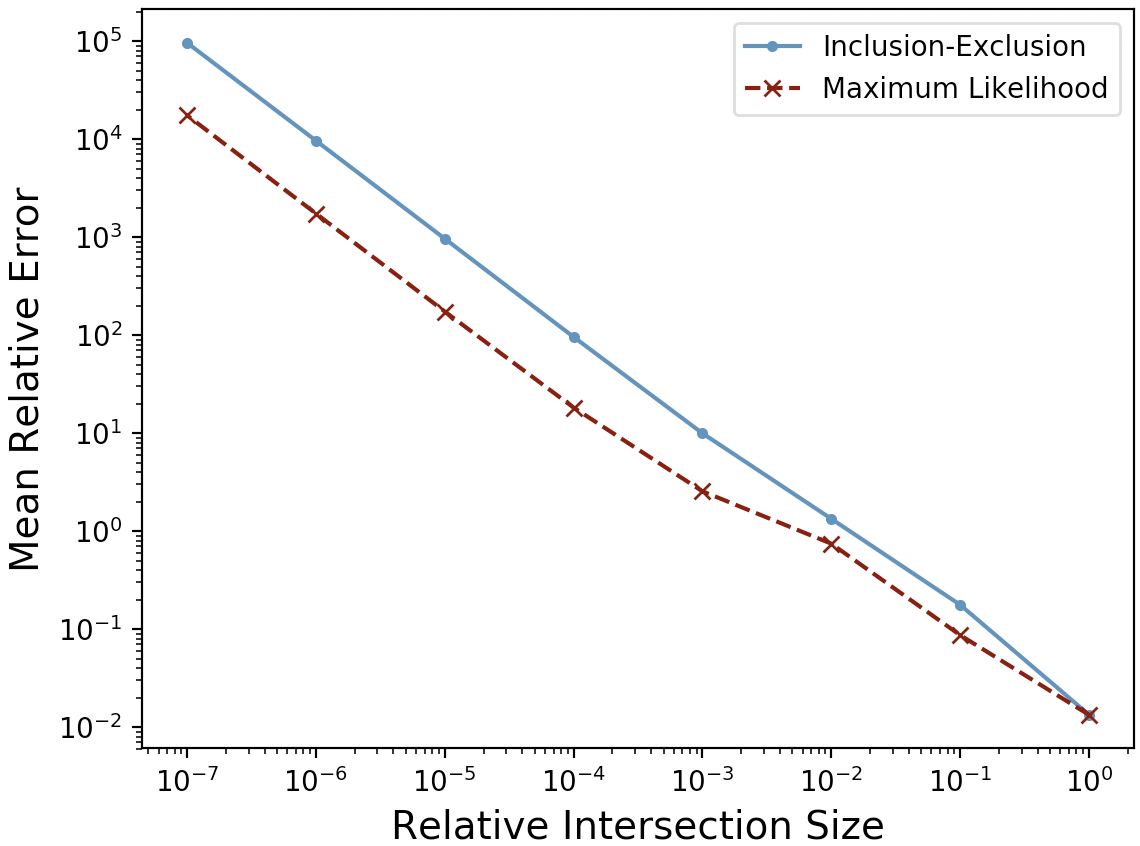
\includegraphics[width=1.0\columnwidth]{relative_intersection_size_vs_relative_error_equal}}
			\caption{$p = 8$. \label{fig:relative_intersection_size_equal_8}}
		\end{subfigure}%
		\hspace{1em}%
		\begin{subfigure}{0.45\linewidth}
			\centerline{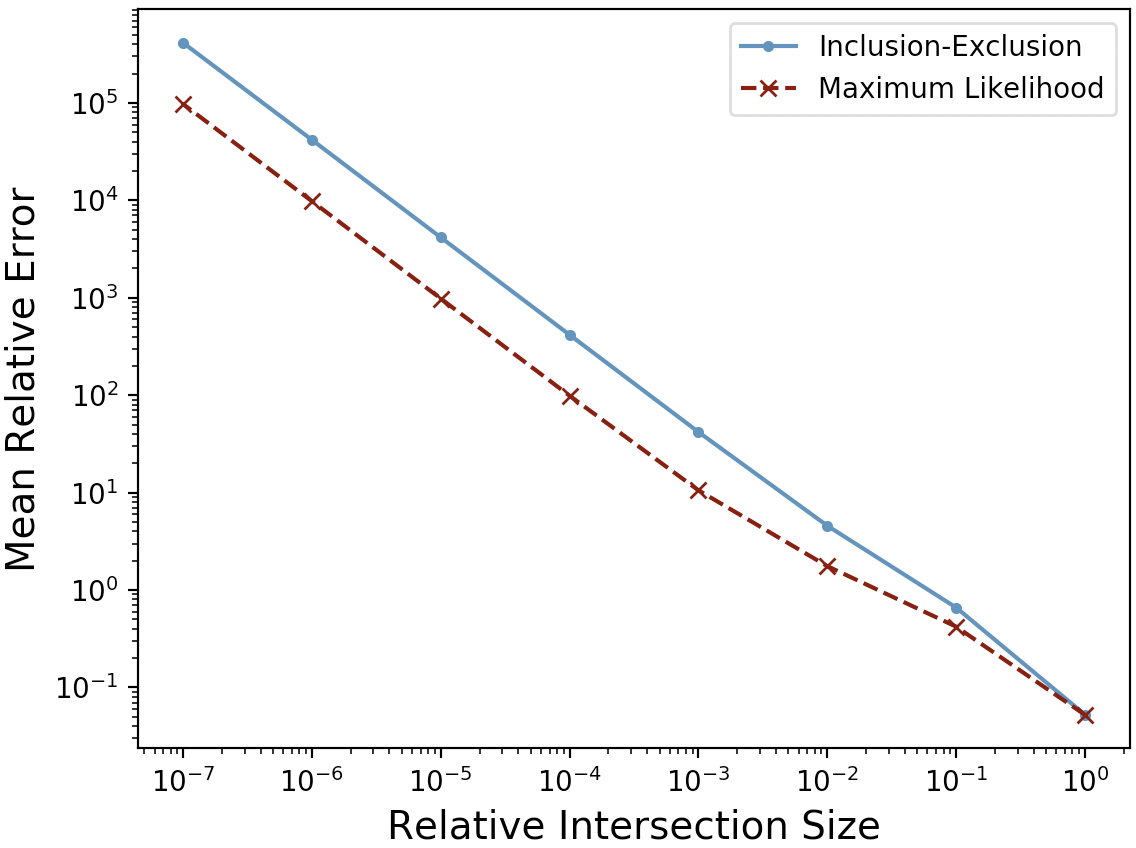
\includegraphics[width=1.0\columnwidth]{relative_intersection_size_vs_relative_error_equal_8}}
			\caption{$p = 12$. \label{fig:relative_intersection_size_equal_12}}
		\end{subfigure}%
%		\begin{subfigure}{0.49\linewidth}
%			\centerline{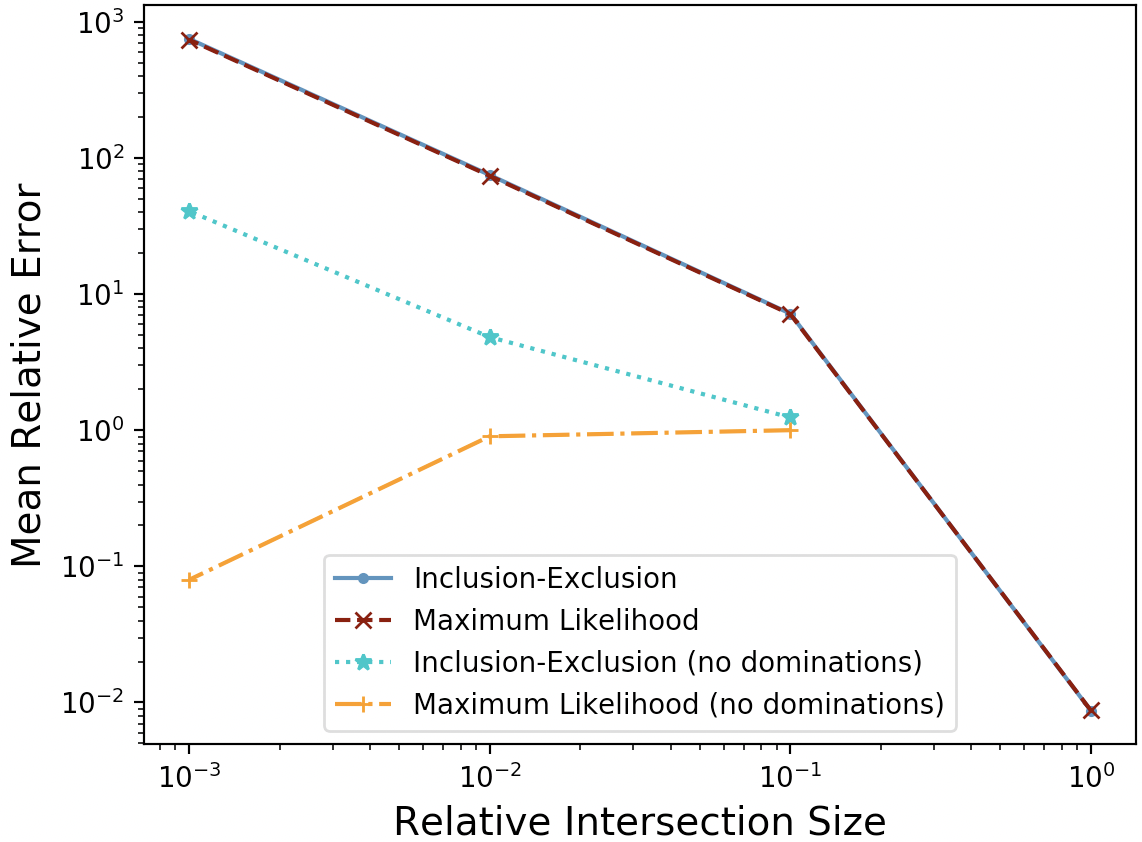
\includegraphics[width=1.0\columnwidth]{relative_intersection_size_vs_relative_error_small}}
%			\caption{Mean relative error as a function of relative intersection size where $|A| = 10^7$ and $|B| = 10^3$. \label{fig:relative_intersection_size_small}}
%		\end{subfigure}
%		\begin{subfigure}{0.49\linewidth}
%			\centerline{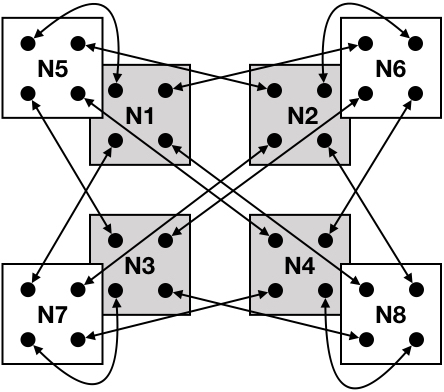
\includegraphics[width=1.0\columnwidth]{inter_layer_nlnr}}
%			\caption{Mean realtive error as a function of $|B|$, where \\ $|A \cap B| = \frac{|B|}{10}$. \label{fig:relative_B_size}}
%		\end{subfigure}
		\caption{\algoname{HLL} inclusion-exclusion and maximum likelihood intersection estimator performance where $|A| = |B| = 10^7$ and $|A \cap B|$ varies from $1$ up to $|B|$.
			Increasing $p$ increases intersection estimator performance.
			\label{fig:relative_intersection_size_equal}}
	\end{center}
\end{figure}


Figure~\ref{fig:relative_intersection_size_equal_8} plots the error of the na\"ive inclusion-exclusion estimator and the maximum likelihood estimator of $|A| = |B| = 10^7$ where $|A \cap B|$ varies from $1$ up to $10^7$ and $p=8$.
The sketches in question then have $r = 2^8 = 256$ registers.
While the maximum likelihood estimator generally outperforms the na\"ive estimator, both exhibit unacceptably poor performance when the true intersection is very small. 
Meanwhile, Figure~\ref{fig:relative_intersection_size_equal_12} plots the same parameters where $p=12$ and so $r = 2^{12} = 4096$.
In particular, the error of the maximum likelihood estimator remains at reasonable levels for much smaller intersections.
The mean relative error remains below 1 up until about the point where $|A \cap B| = \frac{|A|}{10^2}$.

Clearly, performance can clearly be boosted by increasing the precision parameter $p$, thereby increasing the number of registers. 
For fixed set sizes, one can choose $p$ to achieve arbitrarily small precision. 
However, as the sizes of the sets increase a fixed $p$ will cease to suffice, meaning that the size of the sketches is no longer independent of the streaming data size up to logarithmic factors, which is highly undesirable.
Thus, we can expect the triangle counting algorithms such as those described in Sections~\ref{DS:sec:edge_triangles} and \ref{DS:sec:vertex_triangles} to exhibit poor performance when estimating the incident triangles on an edge linking two hubs where the ground truth triangle count is small.
In our implementation on commodity hardware, the maximum likelihood estimations took approximately 2.7732824 times as much time as the na\"ive estimations.

\begin{figure}
	\begin{center}
		\begin{subfigure}{0.49\linewidth}
			\centerline{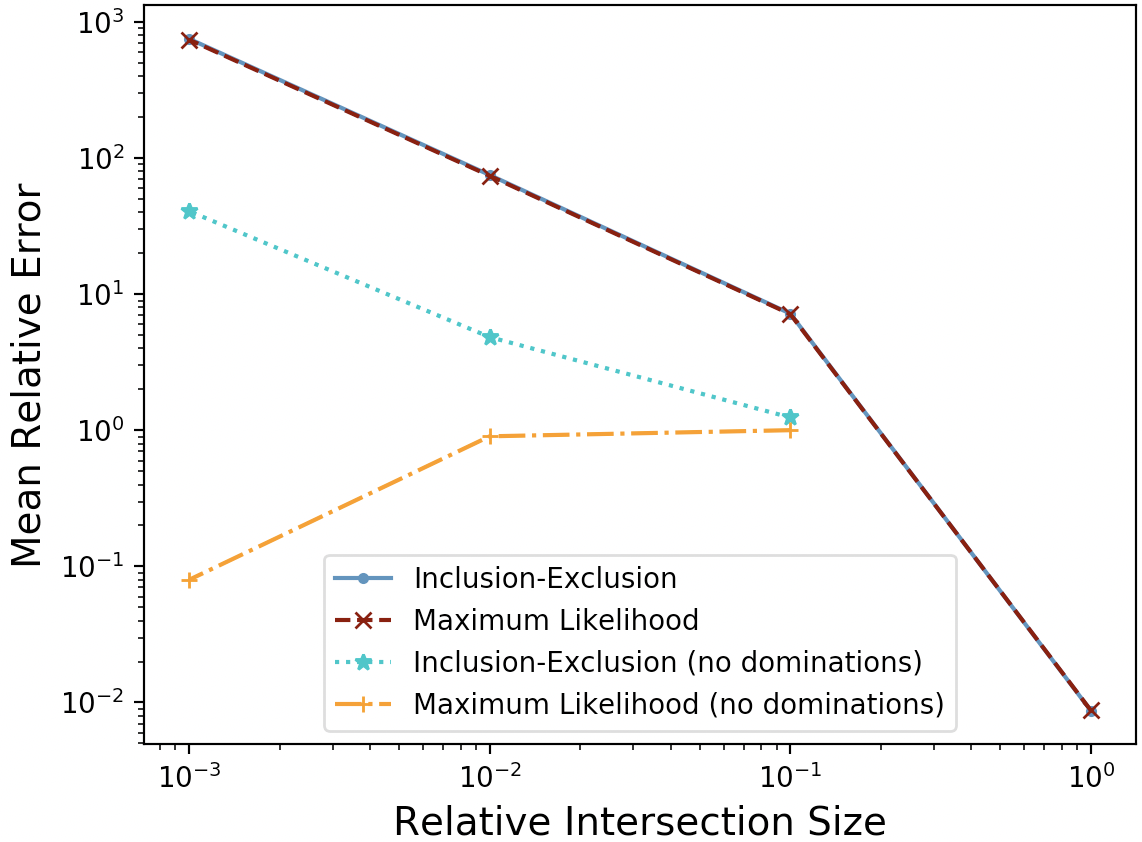
\includegraphics[width=1.0\columnwidth]{relative_intersection_size_vs_relative_error_small}}
			\caption{Mean relative error as a function of relative intersection size where $|A| = 10^7$ and $|B| = 10^3$. \label{fig:relative_intersection_size_small}}
		\end{subfigure}
		\begin{subfigure}{0.49\linewidth}
			\centerline{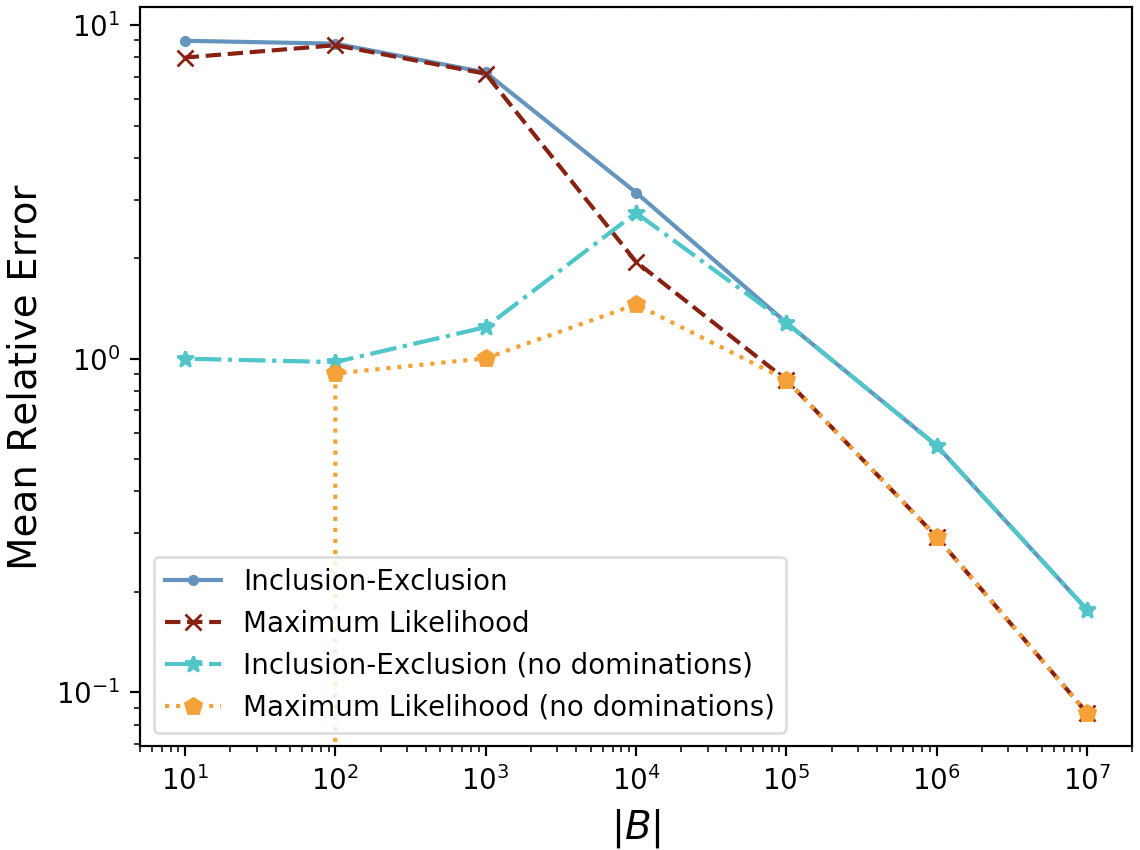
\includegraphics[width=1.0\columnwidth]{B_size_vs_relative_error_tenth_intersection.png}}
			\caption{Mean realtive error as a function of $|B|$, where \\ $|A \cap B| = \frac{|B|}{10}$. \label{fig:relative_B_size}}
		\end{subfigure}
		\caption{More comparisons between \algoname{HLL} inclusion-exclusion and maximum likelihood intersection estimator performance where $|A| = 10^7$ and $p = 12$.
			\label{fig:more_intersection_comparisons}}
	\end{center}
\end{figure}


Meanwhile, Figure~\ref{fig:relative_intersection_size_small} plots the same relationship where $|B| = 10^3 = \frac{|A|}{10^4}$.
This plot shows us a somewhat different picture. 
While both estimators perform poorly when the intersection is small, both appear to consistently estimate the intersection to be $|B| = 10^3$.
This is due to the observation of the effects of dominations from Section~\ref{DS:sec:intersections}.
Firgure~\ref{fig:relative_intersection_size_small} also plots the error of just the comparisons where $A$ does not dominate $B$ at all (about $25\%$ of the experiments). 
%Removing only strict dominations does decrease the mean relative error for both algorithms, but they remain asymptotically equivalent.
Eliminating the strict dominations does not dramatically improve mean performance, which appears asymptotically consistent with the aggregate.
However, removing all estimates that involve a domination results in \emph{improved} performance of both estimators.
In fact, the maximum likelihood estimator actually appears to improve as the intersection size decreases. 
On the other hand, the non-domination inclusion-exclusion estimates appear to exhibit relative error that is better, but not dramatically better, than the domination estimates.

Figure~\ref{fig:relative_B_size} plots the mean relative error as a function of $|B|$, where $|B|$ takes values in $10^j$ for $j \in [7]$ and $|A \cap B|$ is locked to $\frac{|B|}{10}$.
As $|B|$ gets smaller, the likelihood of a domination increases. 
At $|B|= 10^4$ dominations occur in $6.6\%$ of cases, at $|B|= 10^3$ dominations occur in $76.9\%$ of cases, at $|B|= 10^2$ dominations occur in $97.5\%$ of cases, and at $|B|= 10$ dominations occur in $99.8\%$ of cases.
In particular in the two cases where $|B|=10$ and $|A \cap B| = 1$ and a domination does not occur, the maximum likelihood estimator returns exactly 1. 
So for a fixed intersection size relative to $|B|$, both the inclusion-exclusion and maximum likelihood estimators return more reasonable estimates when dominations do not occur.
Figure~\ref{fig:relative_intersection_size_small} indicates that the maximum likelihood estimator benefits more as the intersection decreases. 

These results suggest that, had we a means of avoiding dominations, then the maximum likelihood estimator would be at least coarsely reliable when comparing sets of very different size. 
Unfortunately this is a difficult guarantee to provide.
We can bound the probability that $A$ dominates $B$ for disjoint $A$ and $B$ building from Eqs.~(1) and (2) of \cite{ertl2017new}.
However, the resulting expression is very messy and rather uninformative to look at, so we do not reproduce it here.
Suffice to say that the probability is bounded using the union bound by the normalized sum over all hashings of elements of $A$ and $B$ to their length $r$ register arrays $\mathbf{r}^{(A)}$ and $\mathbf{r}^{(B)}$ of the products of the probabilities that $\mathbf{r}^{(A)}_i \geq \mathbf{r}^{(B)}_i$.
By increasing $r$, we can make this bound arbitrarily small for a given $|A|$ and $|B|$ by doubling the number of registers for each incremental increase in $p$.
A similar expression suffices for the case where $|A \cap B| \neq 0$, but the expression grows even more complex.
However, as $|A \cup B|$ increases the bound also increases.
Ergo, if we want to bound the probability that a domination occurs among disjoint sets of a given sizes, it requires setting $r$ scaling proportional to $|A \cup B|$.
This is clearly an infeasible condition for a streaming algorithm, as the size of the sketch is no longer independent of the size of the streaming data.

If $|A| \gg |B|$, then for a fixed precision $p$ $A$ will asymptotically dominate $B$.
Increasing $p$ may suffice given a ceiling upon the size of the sets, but we have sketched how this is not a valid general purpose solution. 
Unfortunately, this means that unless the size of possible sets has a reasonable bound, it it not feasible to reliably recover intersections of very differently sized sets.

These negative results set a dour tone for our subsequent analysis. 
We have shown that the intersection estimator exhibits poor performance on very small intersections of equally sized sets and the intersections of sets of wildly different sizes, and we have explored why these gaps in performance occur.
Thus, the performance of the algorithms of Sections~\ref{DS:sec:edge_triangles} and \ref{DS:sec:edge_triangles} are dependent upon how prevalent these cases are in the data.
This is the reason that we limit ourselves to empirical heavy hitter recovery.

%----------------------------------------------------------------------------------------
\subsection{Local Triangle Counting}
 \label{DS:sec:experiments:triangles}
%----------------------------------------------------------------------------------------

We performed experiments on real graph datasets for the purpose of establishing the following of our Algorithms.
\begin{enumerate}
	\item \textbf{Heavy Hitter recovery	} Do the heavy hitters returned by Algorithms~\ref{alg:ds:edge_local} and \ref{alg:ds:vertex_local} correspond to the ground truth heavy hitters?
	\item \textbf{Estimation Quality} Do the algorithms yield good global and edge- and vertex-local estimates? How does the maximum likelihood estimator compare to the na\"ive estimator?
	\item \textbf{Speed \& Scalability} How fast is accumulation? Estimation? How does wall time relate to $|\mathcal{P}|$?
\end{enumerate}


%Fortunately, we can report some positive results below.
%Table~\ref{tab:big} lists the performance of Algorithm~\ref{alg:ds:edge_local}, the Edge-Local Triangle Count Heavy Hitters on 58 graphs. 

\noindent
\textbf{Graphs}: 
We considered the graphs listed in Table \ref{tab:graphs}.
We simulated graph streams by randomly ordering and partitioning the edge lists into $|\mathcal{P}|$ separate files, one of which is read by each member of $\mathcal{P}$.

Many of these graphs are provided by Stanford's widely used SNAP dataset \cite{snapnets}.
These graphs are collected from natural sources, such as email records, transportation networks, peer-to-peer communications, social media, and citation corpora, among others.
We casted each graph as unweighted, ignoring directionality, self-loops, and repeated edges. 

We also used 5 graphs derived from nonstochastic Kronecker products of smaller graphs.
Nonstochastic Kronecker graphs \cite{weichsel1962kronecker} have adjacency matrices $C$ that are Kronecker products $C = C_1 \otimes C_2$, where the factors are also adjacency matrices.
This type of synthetic graph is attractive for testing graph analytics at massive scale \cite{leskovec2010kronecker, kepner2018design}, as ground truth solution is often cheaply computable.
For such graphs, global triangle count and triangle counts at edges are computed via Kronecker formulas \cite{sanders2018large}: for a graph with $m$ edges, the worst-case cost of computing global triangle counts is sublinear, $O \left ( m^{\frac{3}{4}} \right )$, whereas the cost of computing the full set of edge-local counts is $O \left ( m \right )$.

Here, we build $C = C_1 \otimes C_2$ from identical factors, $C_1=C_2$, that come from a small set of  graphs with $m$ up to $10^5$ from the University of Florida sparse matrix collection ({\tt polbooks}, {\tt celegans}, {\tt geom}, {\tt yeast} \cite{davis2011university}). 
%, {\tt Oregon-1} -- could not use - catalyst nodes ran out of memory.
All graphs were forced to be undirected, unweighted, and without self loops.  
We compute the number of triangles at each edge for $C_1$ and use the Kronecker formula in \cite{sanders2018large} to get the respective quantities for $C$.
Summing over the edges and dividing by 3 gives the global triangle count for $C$.




\begin{table}[htbp]
\begin{center}
\begin{tabular}{|c|c|c|c|c|c|c|c|}
%\begin{longtable}{|c|c|c|c|c|c|c|c|}
\hline
\textbf{graph} & $|\mathcal{V}|$ & $|\mathcal{E}|$ & $|\mathcal{T}|$ & \textbf{graph} & $|\mathcal{V}|$ & $|\mathcal{E}|$ & $|\mathcal{T}|$  \\
\hline
\hline
as20000102 & 6,474 & 12,572 & 6,584 & 
facebookcombined & 4,039 & 88,234 & 1,612,010  \\
\hline
ca-GrQc & 5,242 & 14,484 & 48,260 & 
p2p-Gnutella30 & 36,682 & 88,328 & 1,590 \\
\hline
p2p-Gnutella08 & 6,301 & 20,777 & 2,383 & 
ca-CondMat & 23,133 & 93,439 & 173,361 \\
\hline
oregon1010407 & 10,729 & 21,999 & 15,834 & 
ca-HepPh & 12,008 & 118,489 & 3,358,500 \\
\hline
oregon1010331 &10,670 &  22,002 & 17,144 & 
p2p-Gnutella31 & 62,586 & 147,892 & 2,024 \\
\hline
oregon1010414 & 10,790 &  22,469 & 18,237 & 
email-Enron & 36,692 & 183,831 & 727,044 \\
\hline
oregon1010428 & 10,886 & 22,493 & 17,645 & 
ca-AstroPh & 18,772 & 198,050 & 1,351,440 \\
\hline
oregon1010505 & 10,943 & 22,607 & 17,597 & 
loc-brightkiteedges & 58,228 & 214,078 & 494,728 \\
\hline
oregon1010512 & 11,011 & 22,677 & 17,598 & 
cit-HepTh & 9,877 & 352,285 & 1,478,740 \\
\hline
oregon1010519 & 11,051 & 22,724 & 17,677 & 
email-EuAll & 265,214 & 364,481 & 267,313  \\
\hline
oregon1010421 & 10,859 & 22,747 & 19,108 & 
\textbf{pb $\boldsymbol{\otimes}$ pb} & 11,024 & 388,962 & 1,881,600 \\
\hline
oregon1010526 & 11,174 & 23,409 & 19,894 & 
soc-Epinions1 & 75,879 & 405,740 & 1,624,480 \\
\hline
ca-HepTh & 9,877 & 25,973 & 28,339 & 
cit-HepPh & 34,546 & 420,877 & 1,276,870 \\
\hline
p2p-Gnutella09 & 8,114 & 26,013 & 2,354 & 
soc-Slashdot0811 & 77,360 & 469,180 & 551,724 \\
\hline
oregon2010407 & 10,729 & 30,855 & 78,138 & 
soc-Slashdot0902 & 82,168 & 504,230 & 602,592 \\
\hline
oregon2010505 & 11,157 & 30,943 & 72,182 & 
amazon0302 & 262,111 & 899,792 & 717,719 \\
\hline
oregon2010331 & 10,900 & 31,180 & 82,856 & 
loc-gowallaedges & 196,591 & 950,327 & 2,273,140 \\
\hline
oregon2010512 & 11,260 & 31,303 & 72,866 & 
roadNet-PA & 1,088,092 & 1,541,898 & 67,150 \\
\hline
oregon2010428 & 11,113 & 31,434 & 78,000 & 
roadNet-TX & 1,379,917 & 1,921,660 & 82,869 \\
\hline
p2p-Gnutella06 & 8,717 & 31,525 & 1,142 & 
flickrEdges & 105,938 & 2,316,948 & 107,987,000 \\
\hline
oregon2010421 & 11,080 & 31,538 & 82,129 & 
amazon0312 & 400,727 & 2,349,869 & 3,686,470 \\
\hline
oregon2010414 & 11,019 & 31,761 & 88,905 & 
amazon0505 & 410,236 & 2,439,437 & 3,951,060 \\
\hline
p2p-Gnutella05 & 8,846 & 31,839 & 1,112 & 
amazon0601 & 403,394 & 2,443,408 & 3,986,510 \\
\hline
oregon2010519 & 1,1375 & 32,287 & 83,709 & 
roadNet-CA & 1,965,206 & 2,766,607 & 120,676 \\
\hline
oregon2010526 & 11,461 & 32,730 & 89,541 & 
graph500-scale18-ef16 & 174,147 & 3,800,348 & 82,287,300 \\
\hline
p2p-Gnutella04 & 10,876 & 39,994 & 934 & 
\textbf{cg $\boldsymbol{\otimes}$ cg} & 205,208 & 8,201,250 & 64,707,900 \\
\hline
as-caida20071105 & 26,475 & 53,381 & 36,365 & 
\textbf{ns $\boldsymbol{\otimes}$ ns} & 2,524,920 & 15,037,128 & 85,006,200 \\
\hline
p2p-Gnutella25 & 22,687 & 54,705 & 806 & 
cit-Patents & 3,774,768 & 16,518,947 & 7,515,020 \\
\hline
p2p-Gnutella24 & 26,518 & 65,369 & 986 & 
\textbf{em $\boldsymbol{\otimes}$ em} & 1,283,688 & 59,426,802 & 171,286,000 \\
\hline
& & & & \textbf{ye $\boldsymbol{\otimes}$ ye} & 5,574,320 & 88,338,632 & 74,765,400 \\
\hline
%\end{longtable}
\end{tabular}
\end{center}
\caption{Considered moderate graphs \label{tab:graphs}}
\end{table}



\noindent
\textbf{Hardware}: 
All of the experiments were performed on a cluster of compute nodes with thirty-six 2.1 GHz Intel Xeon E5-2695 v4 cores and 128GB memory per node. 
We varied the number of nodes per experiment depending on scalability requirements and the size of the graph.
Each core on each node is responsible for an equally sized partition of the vertices in the graph.
We consider graph partitioning to be a separate problem, and accordingly use simple round-robin assignment for our experiments.

\noindent
\textbf{Implementation}:
We implemented all of our algorithms in C++ and MVAPICH2 2.3. 
Inter- and intra-node communication is managed using the pseudo-asynchronous MPI-enabled communication software package YGM described in Chapter~\ref{chap:async}.
% \footnote{put github link here.}.
%Our implementations are freely available on Github \footnote{put github link here.}.
We used xxhash as our hash function implementation \cite{xxhash}. 

\noindent
\textbf{Evaluation}:
We ran each experiment for a total of 100 iterations using different random seeds, using prefix size $p = 12$. 
We found in experiments that this size gave the best tradeoff between performance and accuracy.
We evaluated the accuracy of the estimates of each algorithm in terms of 
%
\begin{align}
\label{eq:global_error}
\text{global relative error} &= \frac{ \left | T - \widetilde{T} \right |}{T}, \\
\label{eq:vertex_mre}
\text{mean relative error (vertices)} &= \frac{1}{|\mathcal{V}|} \sum_{u \in \mathcal{V}} \frac{\left | \mathcal{C}^{\algoname{Tri}}(u) - \widetilde{\mathcal{C}}^{\algoname{Tri}}(u) \right |}{1 + \mathcal{C}^{\algoname{Tri}}(u)}, \text{ and} \\
\label{eq:edge_mre}
\text{mean relative error (edges)} &= \frac{1}{|\mathcal{E}|} \sum_{uv \in \mathcal{E}} \frac{\left | \mathcal{C}^{\algoname{Tri}}(uv) - \widetilde{\mathcal{C}}^{\algoname{Tri}}(uv) \right |}{1 + \mathcal{C}^{\algoname{Tri}}(uv)}
\end{align}
%
as appropriate.
We will abbreviate ``mean relative error'' as MRE in figures and tables.
%We also examine the element-wise relative error distributions in detail in Section~\ref{sec:estimation}.

In addition, we computed the top $k$ ground truth edge- and vertex-local triangle count elements of each graph, and compared them with the estimated top $k$ elements. 
We considered multiple performance metrics using this approach.

One can make a similar comparison to the precision vs recall tradeoff by directly comparing the orderings.
Kendall's rank correlation coefficient, often colloquially referred to as Kendall's $\tau$, is a canonical non-parametric statistic that quantifies the similarity between different indexings of the same data \cite{kendall1938new}.
Vigna generalized Kendall's $\tau$ to a correlation coefficient that is robust to ties within indexings and permits weightings of different indices.
This generalization is an additive hyperbolic weighted correlation coefficient, and we will refer to it as Vigna's $\tau_{h, \phi}$ \cite{vigna2015weighted}.
$\tau_{h, \phi}$ is a correlation coefficient on two indexings $\{s_i\}_{i=1}^n$ and $\{r_i\}_{i=1}^n$ of the set of elements $\{1, 2, \dots, n\}$.
Assume that $\phi : \{1, 2, \dots, n\} \rightarrow \{1, 2, \dots, n, \infty\}$ is the map of elements to their ground truth rank, where $\phi(i) = \infty$ indicates that $i$ has null rank. 
Let
%
\begin{equation} \label{eq:tau_inner}
\langle r, s \rangle_{h, \phi} = \sum_{i < j} \algoname{sgn}(x_i - x_j)\algoname{sgn}(y_i - y_j) \left ( \frac{1}{\phi(i)+ 1} + \frac{1}{\phi(j)+ 1} \right ),
\end{equation}
%
where 
%
\begin{equation} \label{eq:sgn}
\algoname{sgn}(z) \coloneqq 
\begin{cases}
	1 &\text{if $x > 0$}\\
	0 &\text{if $x = 0$}\\
	-1 &\text{if $x < 0$}
\end{cases}. 
\end{equation}
%
If we further define the norm $\| r \|_{h, \phi} = \sqrt{ \langle r, r \rangle_{h, \phi}}$, $\tau_{h, \phi}$ can be expressed as 
%
\begin{equation} \label{eq:tau}
\tau_{h, \phi} = \frac{\langle r, s \rangle_{h, \phi}} {\| r \|_{h, \phi} \| s \|_{h, \phi}}.
\end{equation}
%
This coefficient yields a value $-1 \leq \tau_{h, \phi} \leq 1$, where $\tau_{h, phi} = 1$ indicates perfect agreement and $\tau_{h, phi} = -1$ indicates perfect disagreement between the indexings.
The use of the hyperbolic function ensures that higher ground truth priority elements bear a greater impact upon the correlation. 
We use the ranking function
%
\begin{equation} \label{eq:phi}
\phi_r(z) \coloneqq 
\begin{cases}
	i &\text{if $i \leq r$ and $z$ is the $i$th largest element}\\
	\infty &\text{else}
\end{cases},
\end{equation}
%
using $\tau_{h,\phi_r}$ to measure top $r$ correlation.
Vigna suggests this function in \cite{vigna2015weighted} as a means of performing top-$r$ correlation comparisons.
When one of the indexings is a ground truth ordering and the other is an estimate, $\tau_{h, \phi_r}$ is affected by only the top $r$ estimated elements, as well as the estimated indices of each of the ground truth elements.
This allows us to efficiently compute Vigna's $\tau_{h, \phi_r}$ on massive orderings in a distributed fashion in a single pass in $\widetilde{O}(n)$ time and $\widetilde{O}(1)$ space, where $r$ is treated as a constant.
We used $r = 100$ in our experiments.

\subsubsection{Heavy Hitter Recovery}

For an experiment consisting of a graph $G$, a prefix size $p$, a number of heavy hitters $k$, and a number of estimated heavy hitters $k^\prime$, we run an implementation of Algorithm~\ref{alg:ds:edge_local} using HyperLogLog sketches with $m=2^p$ registers and accumulate a $k^\prime$-min-heap $\widetilde{H}_{k^\prime}$. 
We then compare this heap to $H_k$, the true set of top $k$ triangle count edges in $G$.
We can also compare $\widetilde{\mathcal{T}}$ to $\mathcal{T}$.

We treat $H_{k^\prime}$ as a one-class classifier of the top $k$ elements in $H_k$, implicitly labelling all other vertices as ``not heavy hitters''.
Accordingly, an edge $e \in \mathcal{E}$ is a true positive (TP) if $e \in H_{k}$ and $e \in \widetilde{H}_{k^\prime}$, a false negative (FN) if $e \in H_{k}$ and $e \not\in \widetilde{H}_{k^\prime}$, a false positive (FP) if $e \not\in H_{k}$ and $e \in \widetilde{H}_{k^\prime}$, or a true negative (TN) if $e \not\in H_{k}$ and $e \not\in \widetilde{H}_{k^\prime}$.
We can report the quality of an experiment in terms of its recall $\left ( \frac{TP}{TP + FN} \right )$ versus its precision $\left ( \frac{TP}{TP + FP} \right )$.
%These are standard measures in information extraction.
The precision versus recall tradeoff is a common metric in information retrieval, where the goal is to tune model parameters so as to force both the precision and recall as close to one as possible.
In our experiments, we vary $k^\prime$ around a stationary $k$ to demonstrate the tradeoffs of accumulating more or less than the target number of heavy hitters.
Although these measures are know to exhibit bias, they are accepted as being reasonable for heavily uneven classification problems such as ours, where the class of interest is a small proportion of the samples \cite{boughorbel2017optimal}. 

\begin{figure}
	\centerline{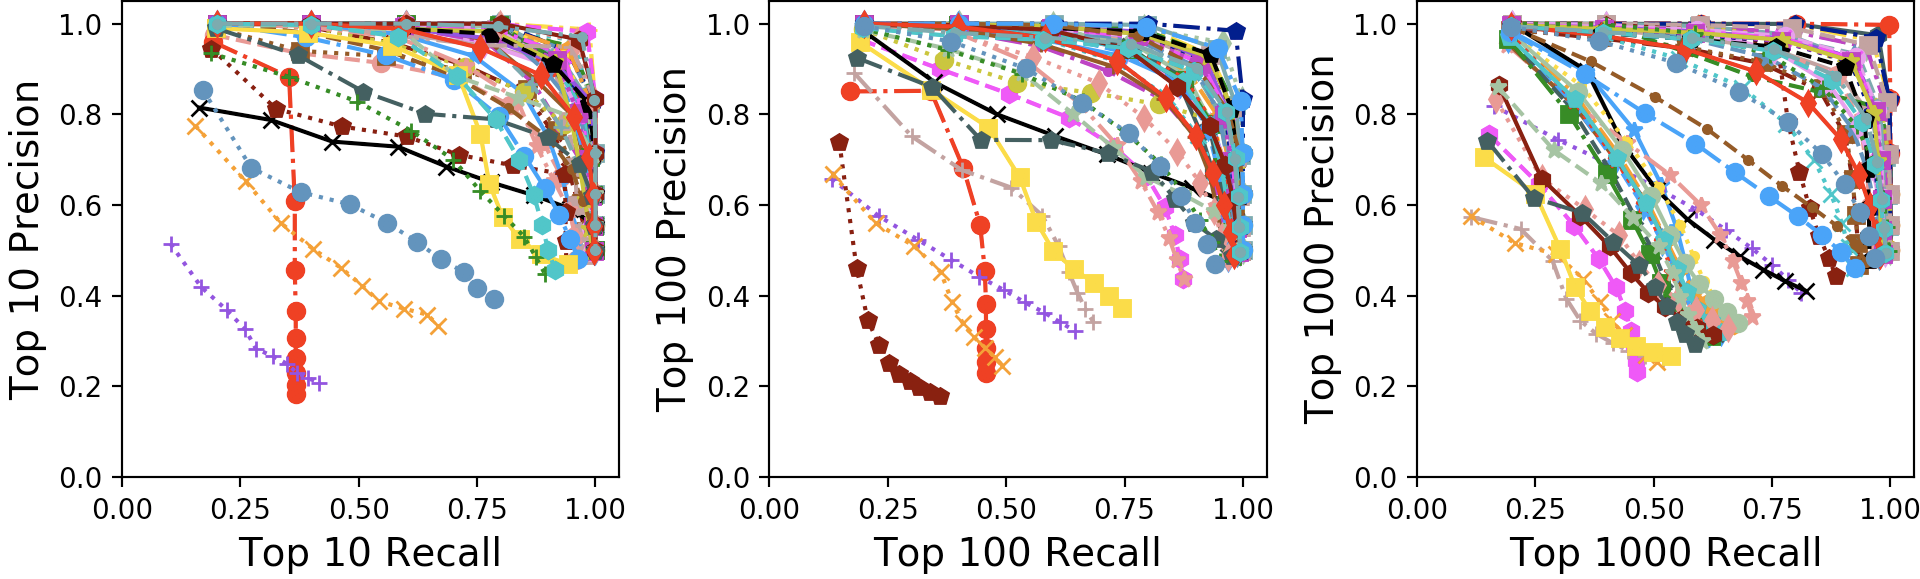
\includegraphics[width=1.0\columnwidth]{graph_challenge_plot}}
	\caption{Precision vs. recall and mean relative error (MRE) for the top 10, top 100, and top 1000 ground truth heavy hitters of all graphs listed in Table~\ref{tab:graphs} using $p=12$ and the na\"ive estimator.
	Also plots the mean relative error for the global estimates and the top 10 false positives and false negatives.
	All mean relative error plots use $k^\prime = k$.
	\label{fig:graph_challenge}}
\end{figure}

Figure~\ref{fig:graph_challenge} shows the edge local precision versus recall curves for all of the graphs in Table~\ref{tab:graphs} for $k = 10, 100, 1000$, where we vary $k^\prime$ from $0.2k$ to $2k$. 
These figures are generated using the na\"ive estimator.
The figure also plots the mean relative error of these top 10, top 100, and top 1000 edges.
They also plot the global mean relative error and the mean relative errors of the false positives and the false negatives.
This false positive relative error is the mean error observed by false positives - edges that are incorrectly identified as heavy hitters.
Similarly, the false negative relative error is the mean error observed by false negatives -edges that the algorithm fails to correctly identify as heavy hitters. 
Low false positive error indicates that the true heavy hitters are still accurately estimated, while low false negative error indicates that those edges falsely identified as top $k^\prime$ elements are still
These results were published by Priest, Pearce and Sanders in \cite{priest2018estimating}.



Figure~\ref{fig:graph_challenge} indicates that while the edge-local algorithm returns good performance on heavy hitter recovery for many of these graphs, some exhibit poor performance.
Figure~\ref{fig:hh_comp} compares three of these poor performers (em $\otimes$ em, p2pGnutella24, and ca-HepTh) with a graph that exhibits good performance (cit-Patents).
The figure plots the triangle count for the ordered top $10^4$ edges in each graph, as well as the triangle density for the same edges, in the same order.
The cit-Patent graph demonstrates near-optimal features of a graph given our approach.
The triangle count distribution is roughly scale-free, making it easier to differentiate top $k$ elements from others for small $k$. 
Furthermore, the triangle density of most of these edges is nontrivial, avoiding the noted problem stemming from estimating small intersections. 
We will discuss how the other three graphs fail to 

Consider first the the em $\otimes$ em graph. 
This is a synthetic kronecker graph, whose formula tends to promote the jagged triangle count distribution seen in Figure~\ref{fig:hh_comp}.
This results in many triangle count ties, which is problematic for our analysis. 
Indeed, this is a weakness of the approach.
Furthermore, all of the heavy hitter edges exhibit low triangle density, with the majority being trivial. 
This leads to increased estimation error as discussed in Section~\ref{DS:sec:intersections}, which can be observed in Figure~\ref{fig:graph_challenge}.
This error exacerbates the problems introduced by having many ties.

Now consider the p2p-Gnutella24 graph. 
This graph also exhibits many ties, but this is due to extreme sparsity of triangles present in the graph. 
Indeed, all but 14 edges in the graph have 2 or fewer incident triangles, and nearly all edges exhibit trivial triangle density.
This graph also exhibits the most estimation error of those considered in our experiments for this reason.
This indicates that our approach is probably not suitable for graphs with very few triangles.
It is worth noting, however, that we are reliably able to capture the top 2 triangle count elements. 

Finally, consider the ca-HepTh graph, which encodes the collaboration network of the Arxiv high energy physics theory community.
This graph, a union of cliques, proves to be a pathological for this problem. 
Note that, save the top 2 edges, the top $\sim 300$ edges are tied in triangle count.
Although our algorithm is able to reliably recover these top 2 elements, even an algorithm with perfect accuracy would fail up to ties on this graph for $k >2$ and $k < \sim 300$, which our results reflect.
Indeed, Figure~\ref{fig:graph_challenge} indicates that this graph exhibits some of the lowest relative error in our experiments.
This indicates that, even for graphs with favorable triangle density, ties can lead to poor heavy hitter recovery. 
This problem could be partially ameliorated via a dynamically sized heap like that utilized in Theorem~\ref{thm:dchh:cashregister}.
%However, this would still be thwarted by near-regular local triangle count graphs like ca-HepTh if size.


\begin{figure}
	\centerline{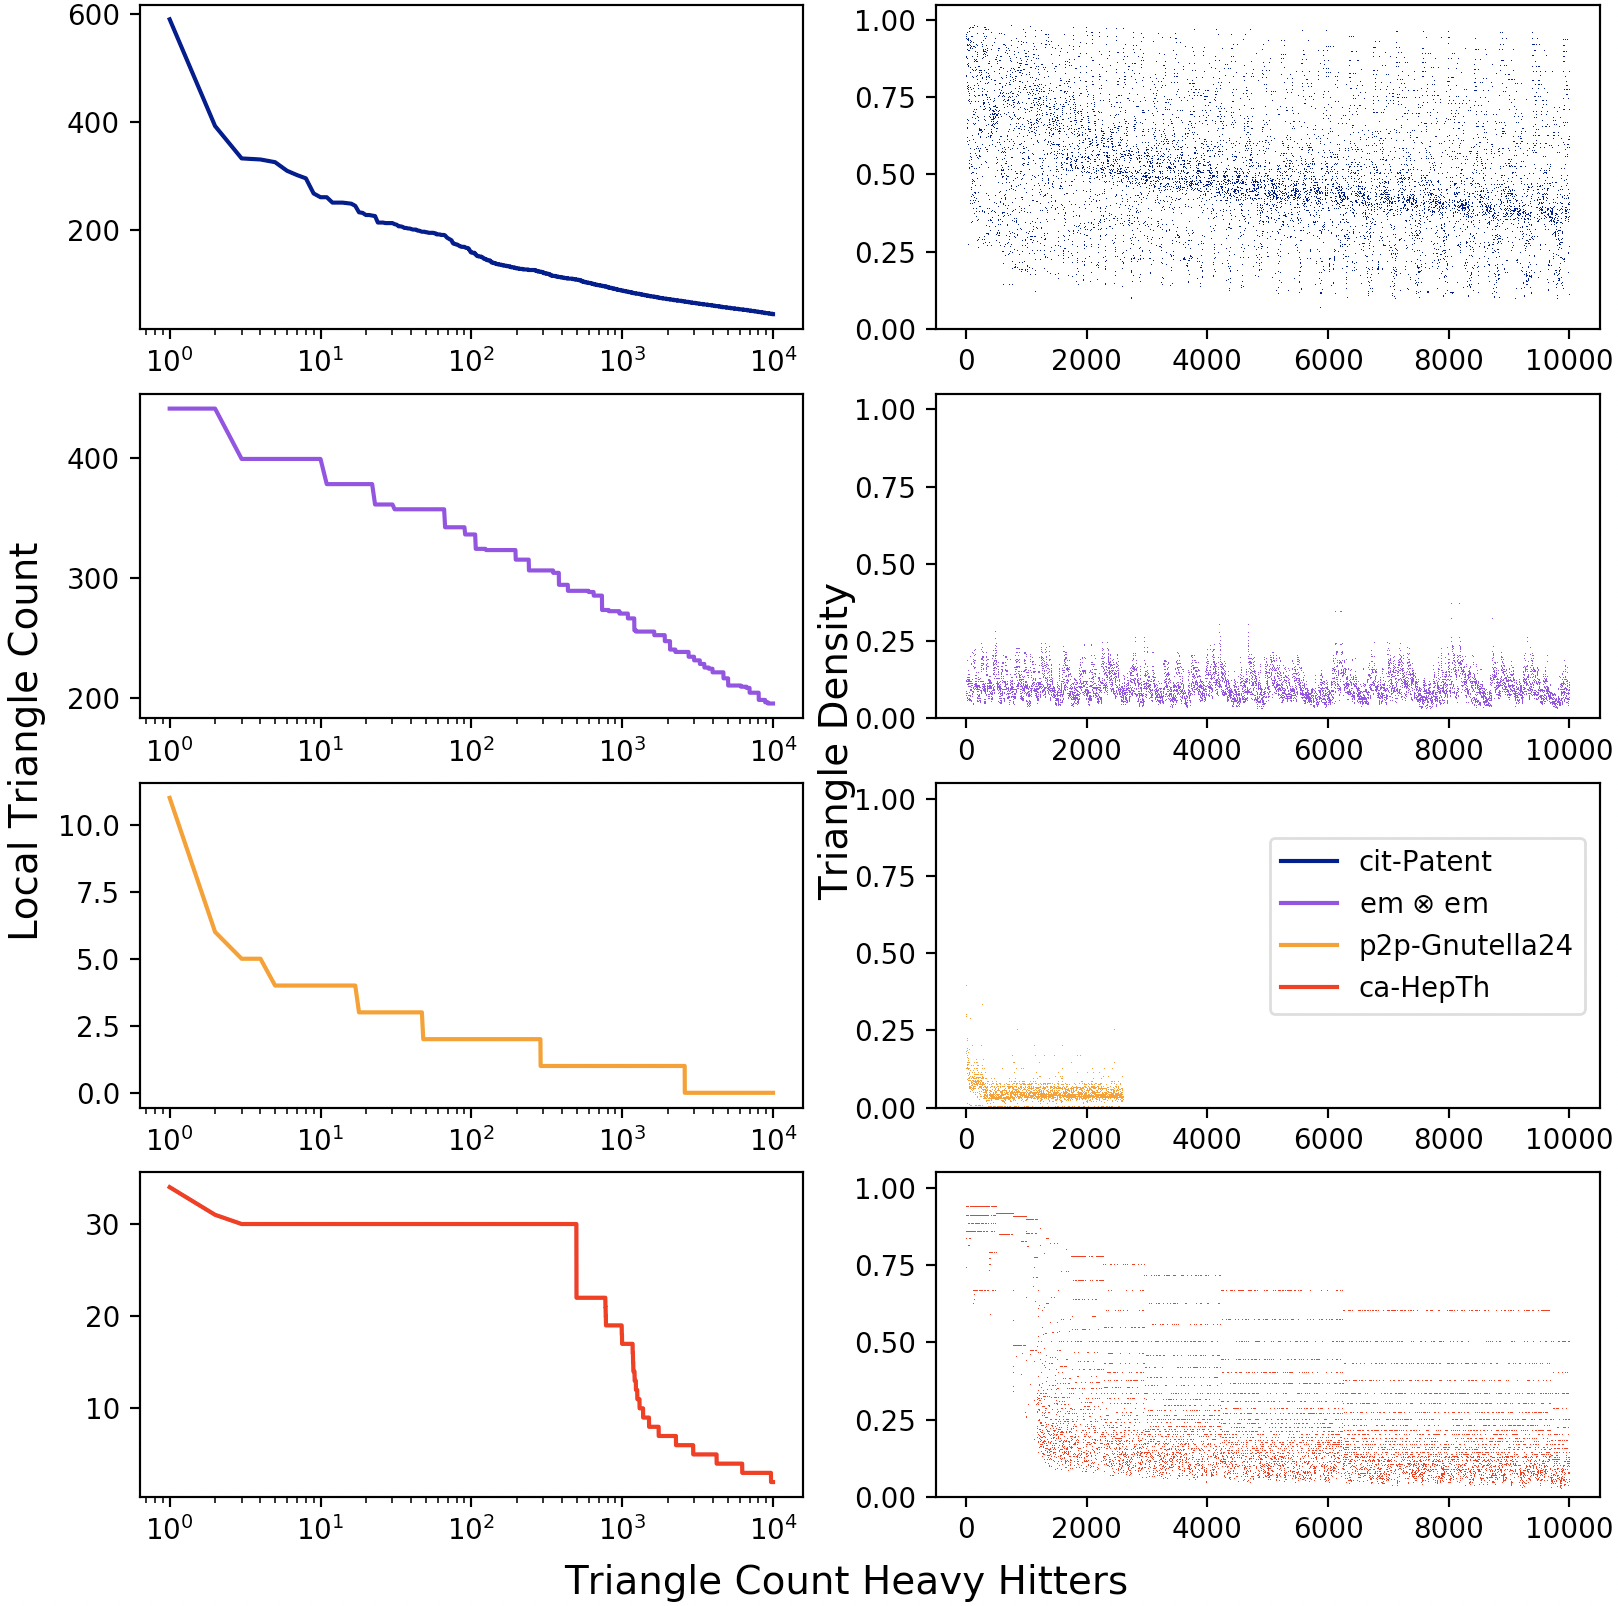
\includegraphics[width=1.0\columnwidth]{hh_comp_4}}
	\caption{The triangle counts and triangle densities of the edge-local triangle count heavy hitters up to $10^4$ for four graphs.
	The cit-Patent graph exhibits good performance in Figure~\ref{fig:graph_challenge}, and demonstrates a reasonable triangle count distribution as well as high triangle density throughout.
	The other three graphs demonstrate poor performance in Figure~\ref{fig:graph_challenge}.
	The kronecker em $\otimes$ em graph exhibits an unusual number of ties in its triangle count distribution due to its construction, in addition to low triangle density among its heavy hitters.
	The P2P-Gnutella24 graph has very low triangle density, and a 3 or fewer triangles for the vast majority of its edges.
	The ca-HepTh graph exhibits an unusual triangle distribution, where a huge portion of its edges tie at 30 triangles.
	Consequently, even a perfect heavy hitter extraction procedure will fail on this graph.
	Notably, the two edges with the largest triangle counts are reliably returned.
	\label{fig:hh_comp}}
\end{figure}

Figure~\ref{fig:graph_challenge} also tells us that as $k$ increases, the relative estimation error of the top $k$ elements tends to increase.
This is sensible, as both the true triangle counts and triangle density tend to decrease as we begin to consider smaller elements.
It is worth noting that some of these graphs would exhibit better performance for different settings of $k$, such as noted p2p-Gnutella and ca-HepTh perform well when $k=2$, because the top two elements stand out above the others.
Unfortunately, in practice we typically cannot know how many outliers there are ahead of time.

Furthermore, the global mean relative error for most of these graphs is reasonable. 
However, there are some notable outliers, which are mostly overestimates due to many small intersections. 
We will show that the maximum likelihood estimator dramatically increases the estimation accuracy in practice.

\subsubsection{Performance comparison between MLE and na\"ive estimators}

We have shown some results concerning the na\"ive estimators. 
It is interesting to compare the performance of the na\"ive estimator to the noted superior performance of the MLE estimator.

We choose to present the results in terms of the distribution of signed error for vertices and edges. 
The signed error of edges and vertices are given by
%
\begin{align}
\label{eq:vertex_sre}
\text{signed relative error (vertex $x$)} &= \frac{\widetilde{\mathcal{C}}^{\algoname{Tri}}(x) - \mathcal{C}^{\algoname{Tri}}(x)}{1 + \mathcal{C}^{\algoname{Tri}}(x)}, \text{ and} \\
\label{eq:edge_sre}
\text{signed relative error (edge $xy$)} &= \frac{\widetilde{\mathcal{C}}^{\algoname{Tri}}(xy) - \mathcal{C}^{\algoname{Tri}}(xy)}{1 + \mathcal{C}^{\algoname{Tri}}(xy)}.
\end{align}
%
The signed error of edge $xy$ varies from -1, where $\widetilde{\mathcal{C}}^{\algoname{Tri}}(xy)$ is incorrectly zero, to $\min \{ \mathbf{d}_x, \mathbf{d}_y \}$, where $\widetilde{\mathcal{C}}^{\algoname{Tri}}(x) = 0$ and a domination occurs, in which case the returned estimate is $\min \{ \mathbf{d}_x, \mathbf{d}_y \}$.
The signed error of a vertex $x$ is similarly bounded above by $\frac{1}{2} \sum_{y : xy \in \mathcal{E}} \min \{\mathbf{d}_x, \mathbf{d}_y \}$.

We ran two experiments of Algorithms~\ref{alg:ds:edge_local} and \ref{alg:ds:vertex_local} on the graphs in Table~\ref{tab:graphs}, disregarding loc-brightkite and loc-gowalla, one using the na\"ive estimator and another using the maximum likelihood estimator.
We used $p=12$ for each experiment. 
We collected the distribution of signed relative error for vertices and edges in each experiment.
As there are a huge number of observations of each phenomenon in each experiment, we only ran each experiment once.



\begin{figure}
	\centerline{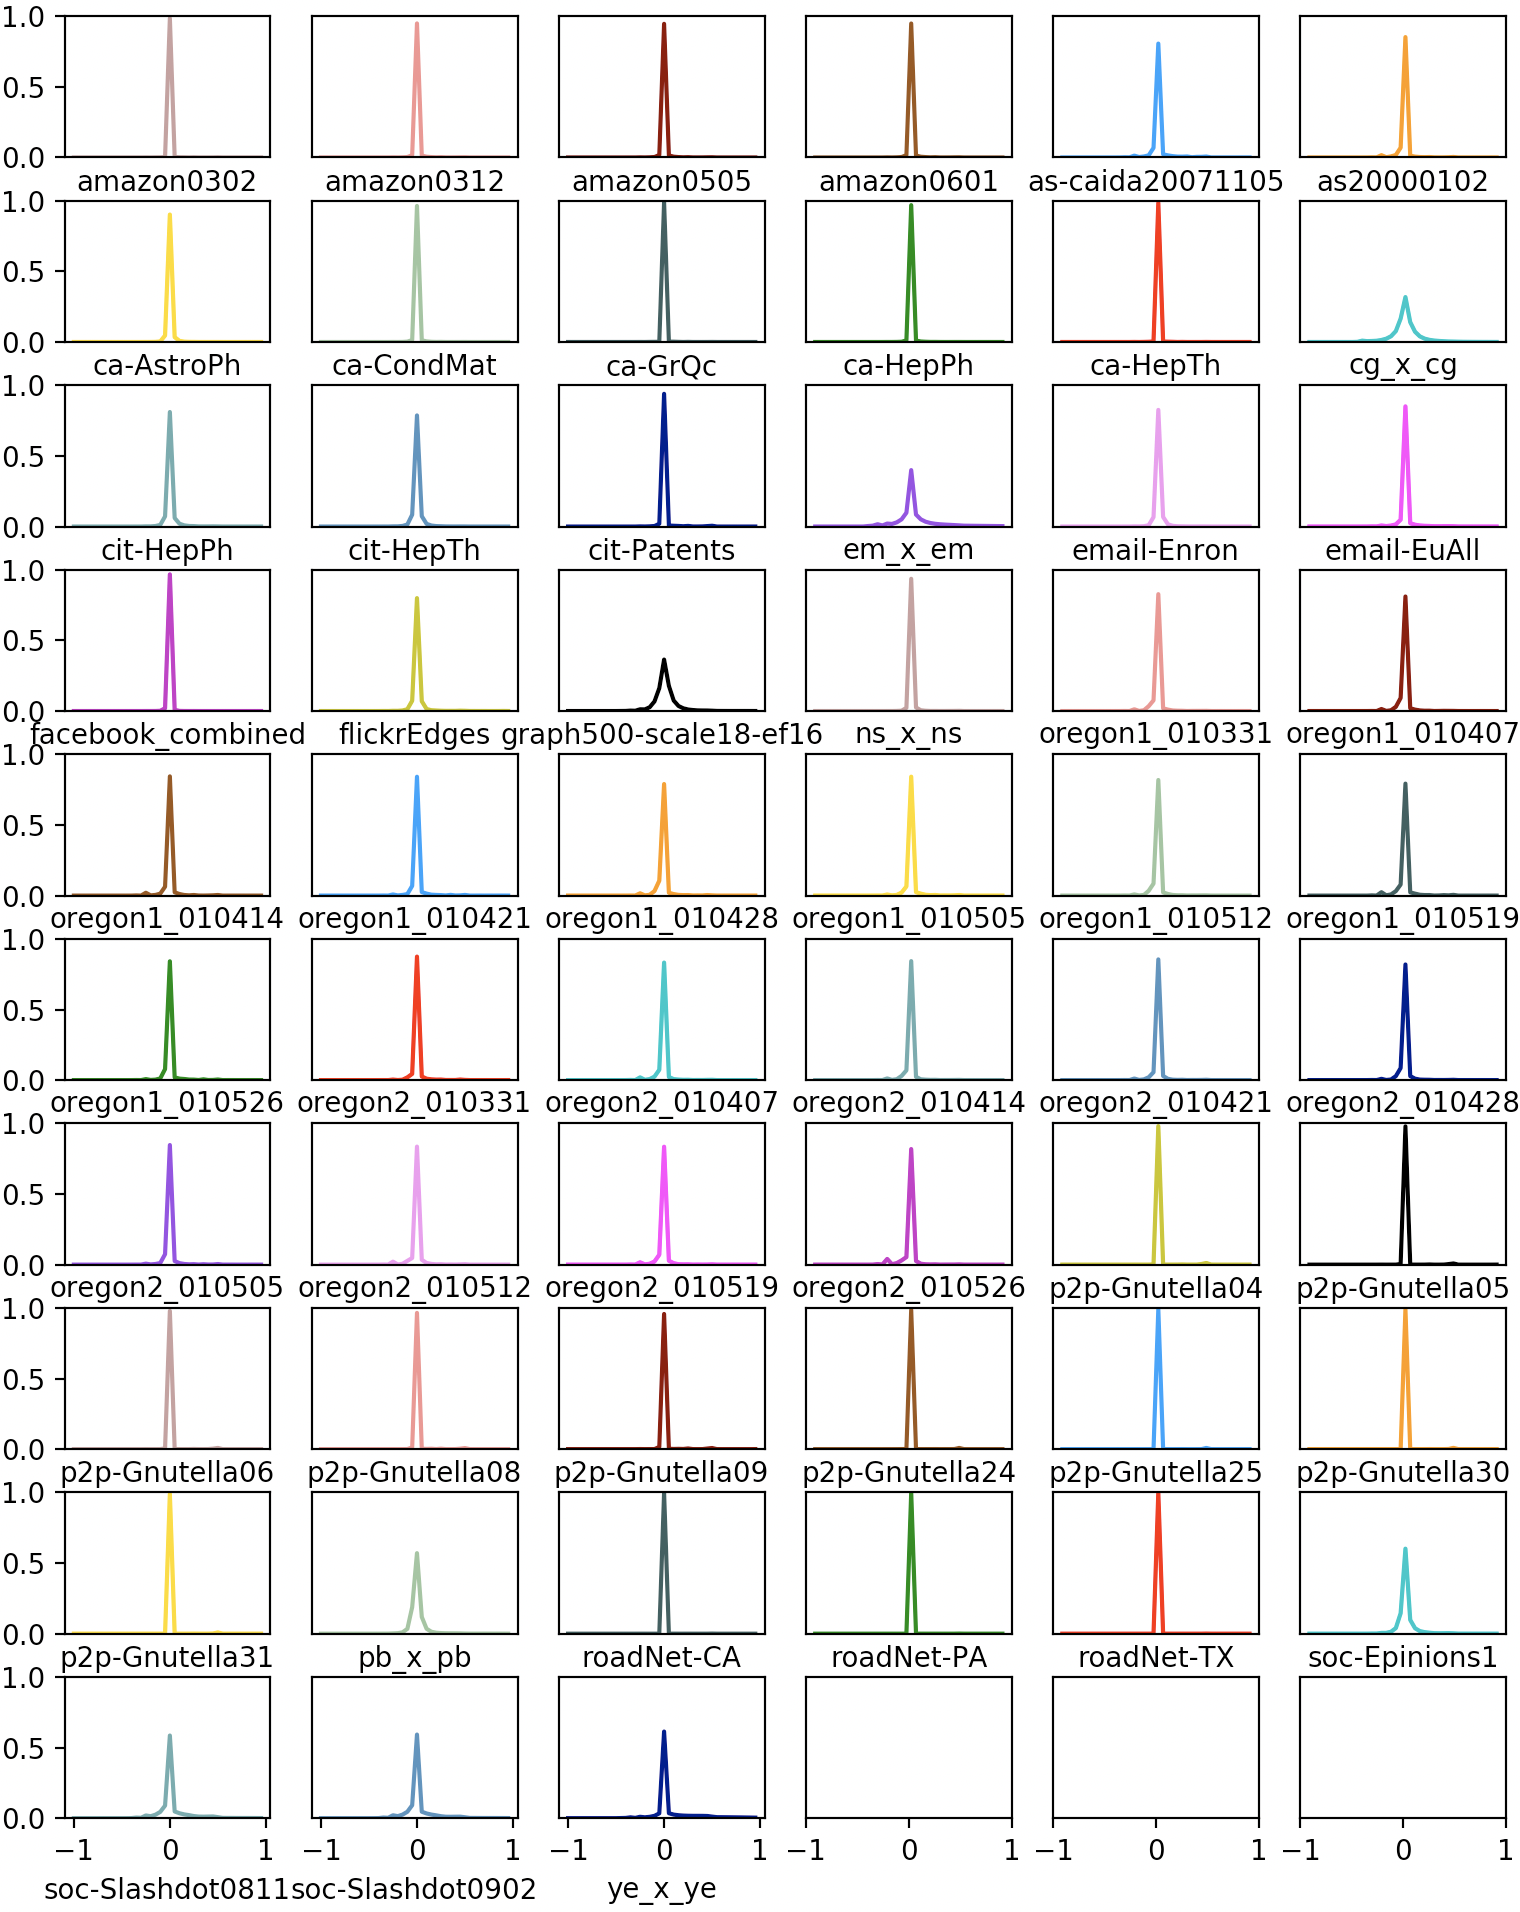
\includegraphics[width=1.0\columnwidth]{distn_edge_total}}
	\caption{The edge-local relative error of most of the  Table~\ref{tab:scaling_graphs} using $p=12$.
	Note that the experimental error appears to be largely unbiased.
	\label{fig:distn_edge}}
\end{figure}

\begin{figure}
	\centerline{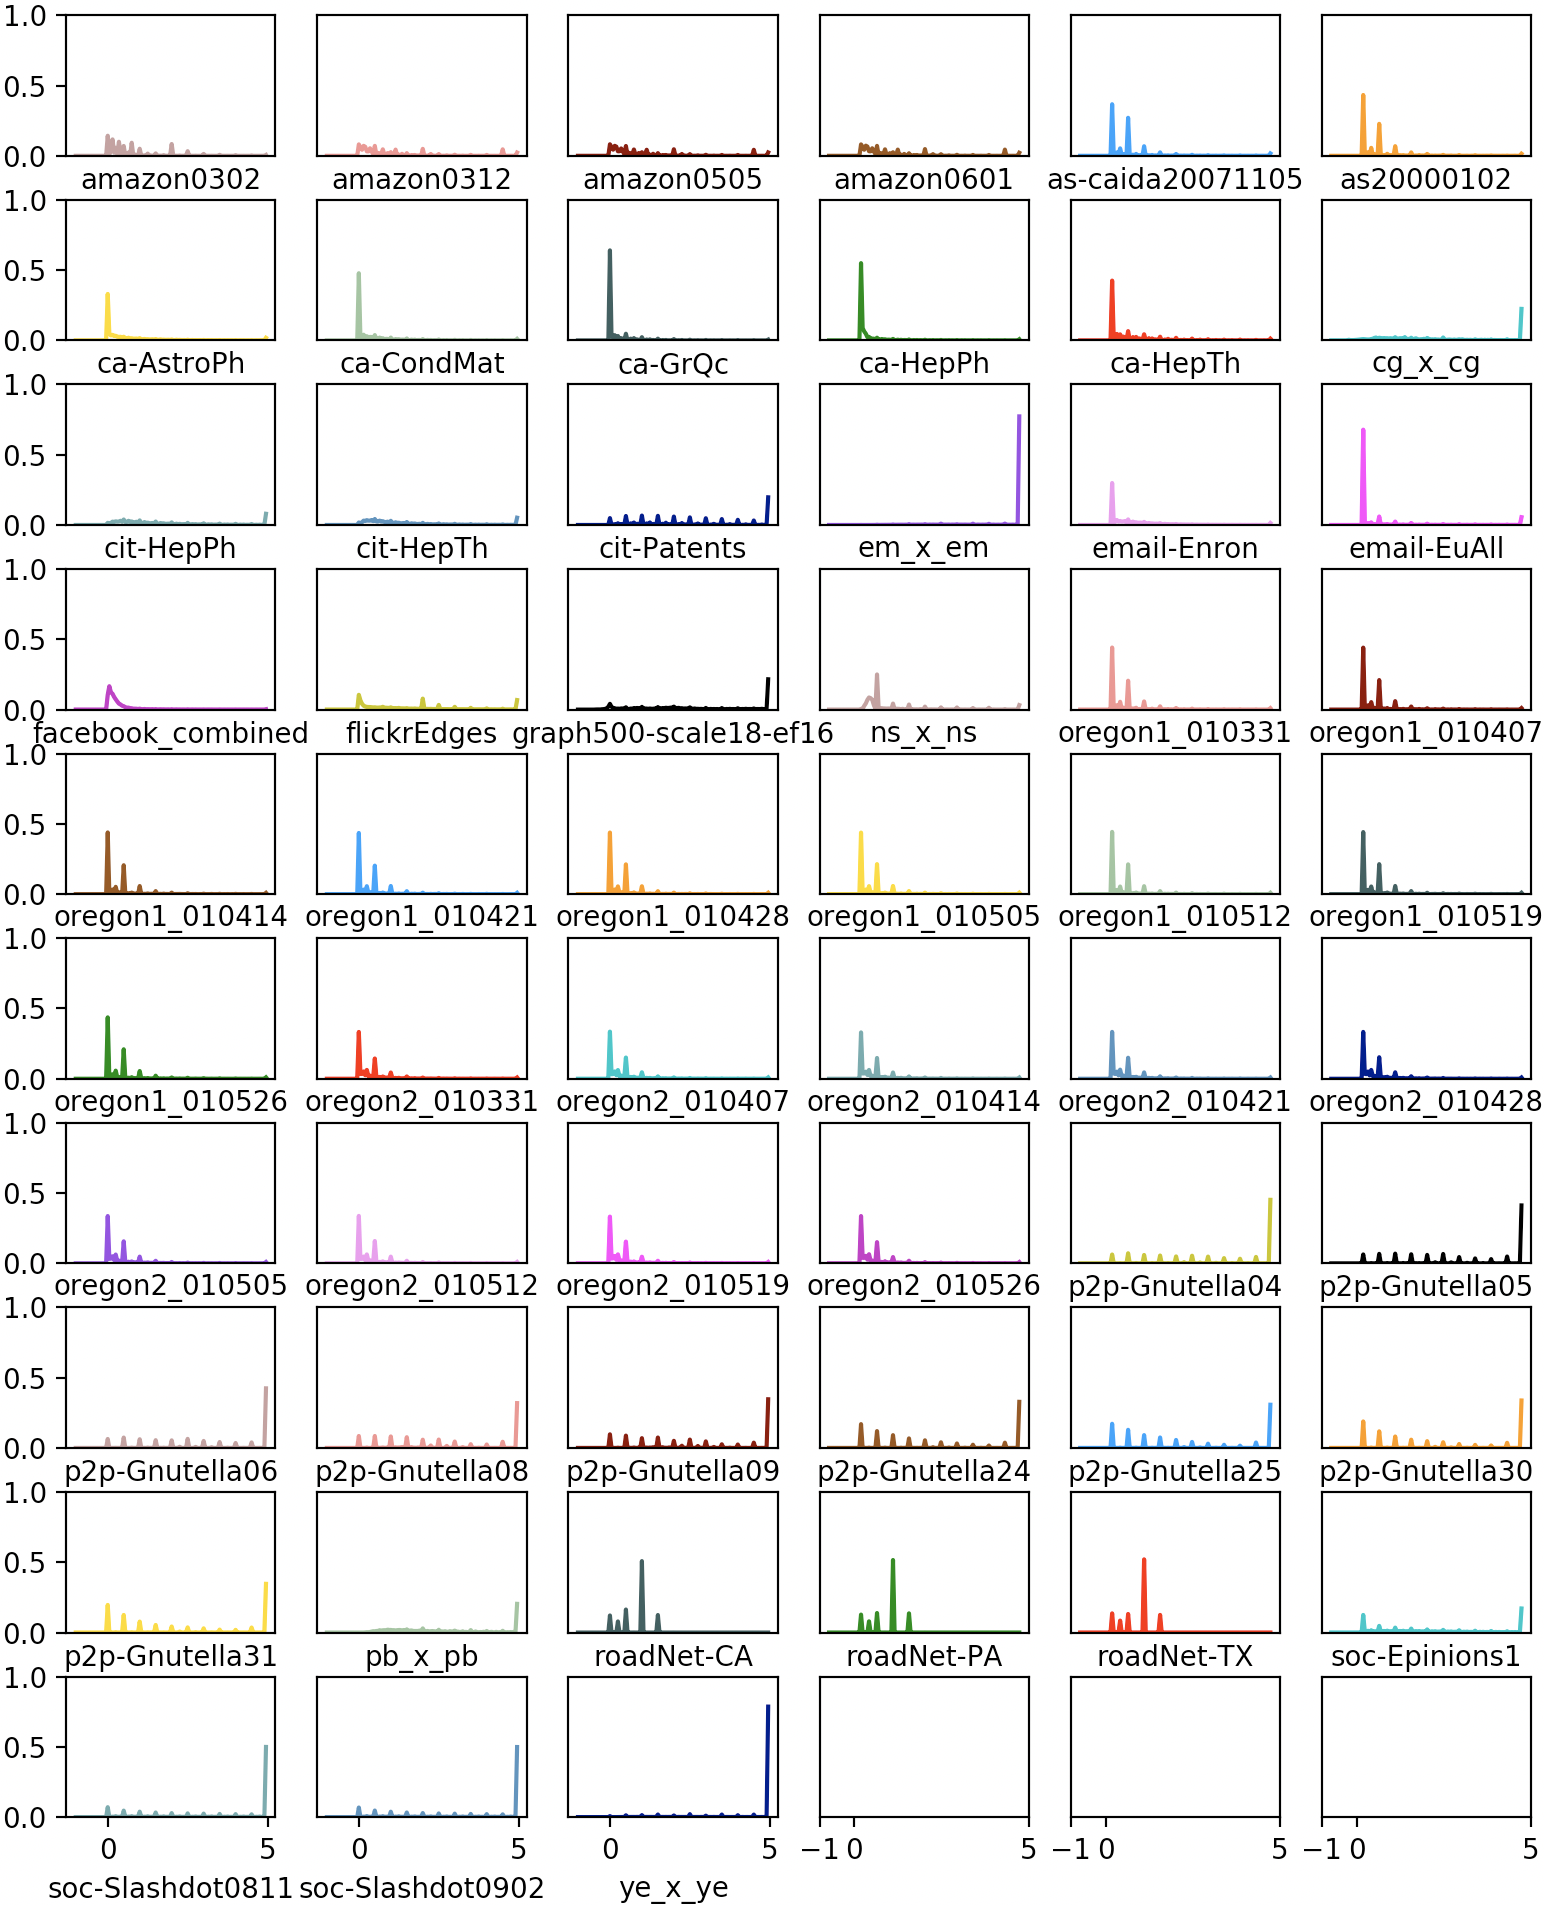
\includegraphics[width=1.0\columnwidth]{distn_naive_edge_total}}
	\caption{The edge-local relative error of most of the  Table~\ref{tab:scaling_graphs} using $p=12$ and the na\"ive inclusion-exclusion intersection estimator. 
	Note that we have had to widen horizontal axis to account for large overestimates in graphs. 
	Note the degraded performance compared to Figure~\ref{fig:distn_edge}.
	\label{fig:distn_naive_edge}}
\end{figure}


Figure~\ref{fig:distn_edge} plots the distributions of edge local signed errors for the graphs using the maximum likelihood estimator. 
Note that the experimental distributions for all vertices appear roughly unbiased around 0, which is highly desirable.
Compare these results with those of the na\"ive inclusion-exclusion estimator in Figure~\ref{fig:distn_naive_edge}.
We have widened the horizontal axis to account for signed error larger than 1.
The jaggedness of the distributions is due to the fact that we round our approximations to the nearest integer.
Note that a few plots have spikes at 5. 
This is because 5 is the largest histogram bucket that we maintained in our experiments, and so anything larger than 5 gets counted as 5. 
In any case, these plots indicate that not only are the na\"ive results biased in most observed graphs, but also they have a propensity to severely overestimate edge local triangle counts.
Thus, the MLE estimator is much more reliable for estimation in general, and can also be used for heavy hitter recovery.


\begin{figure}
	\centerline{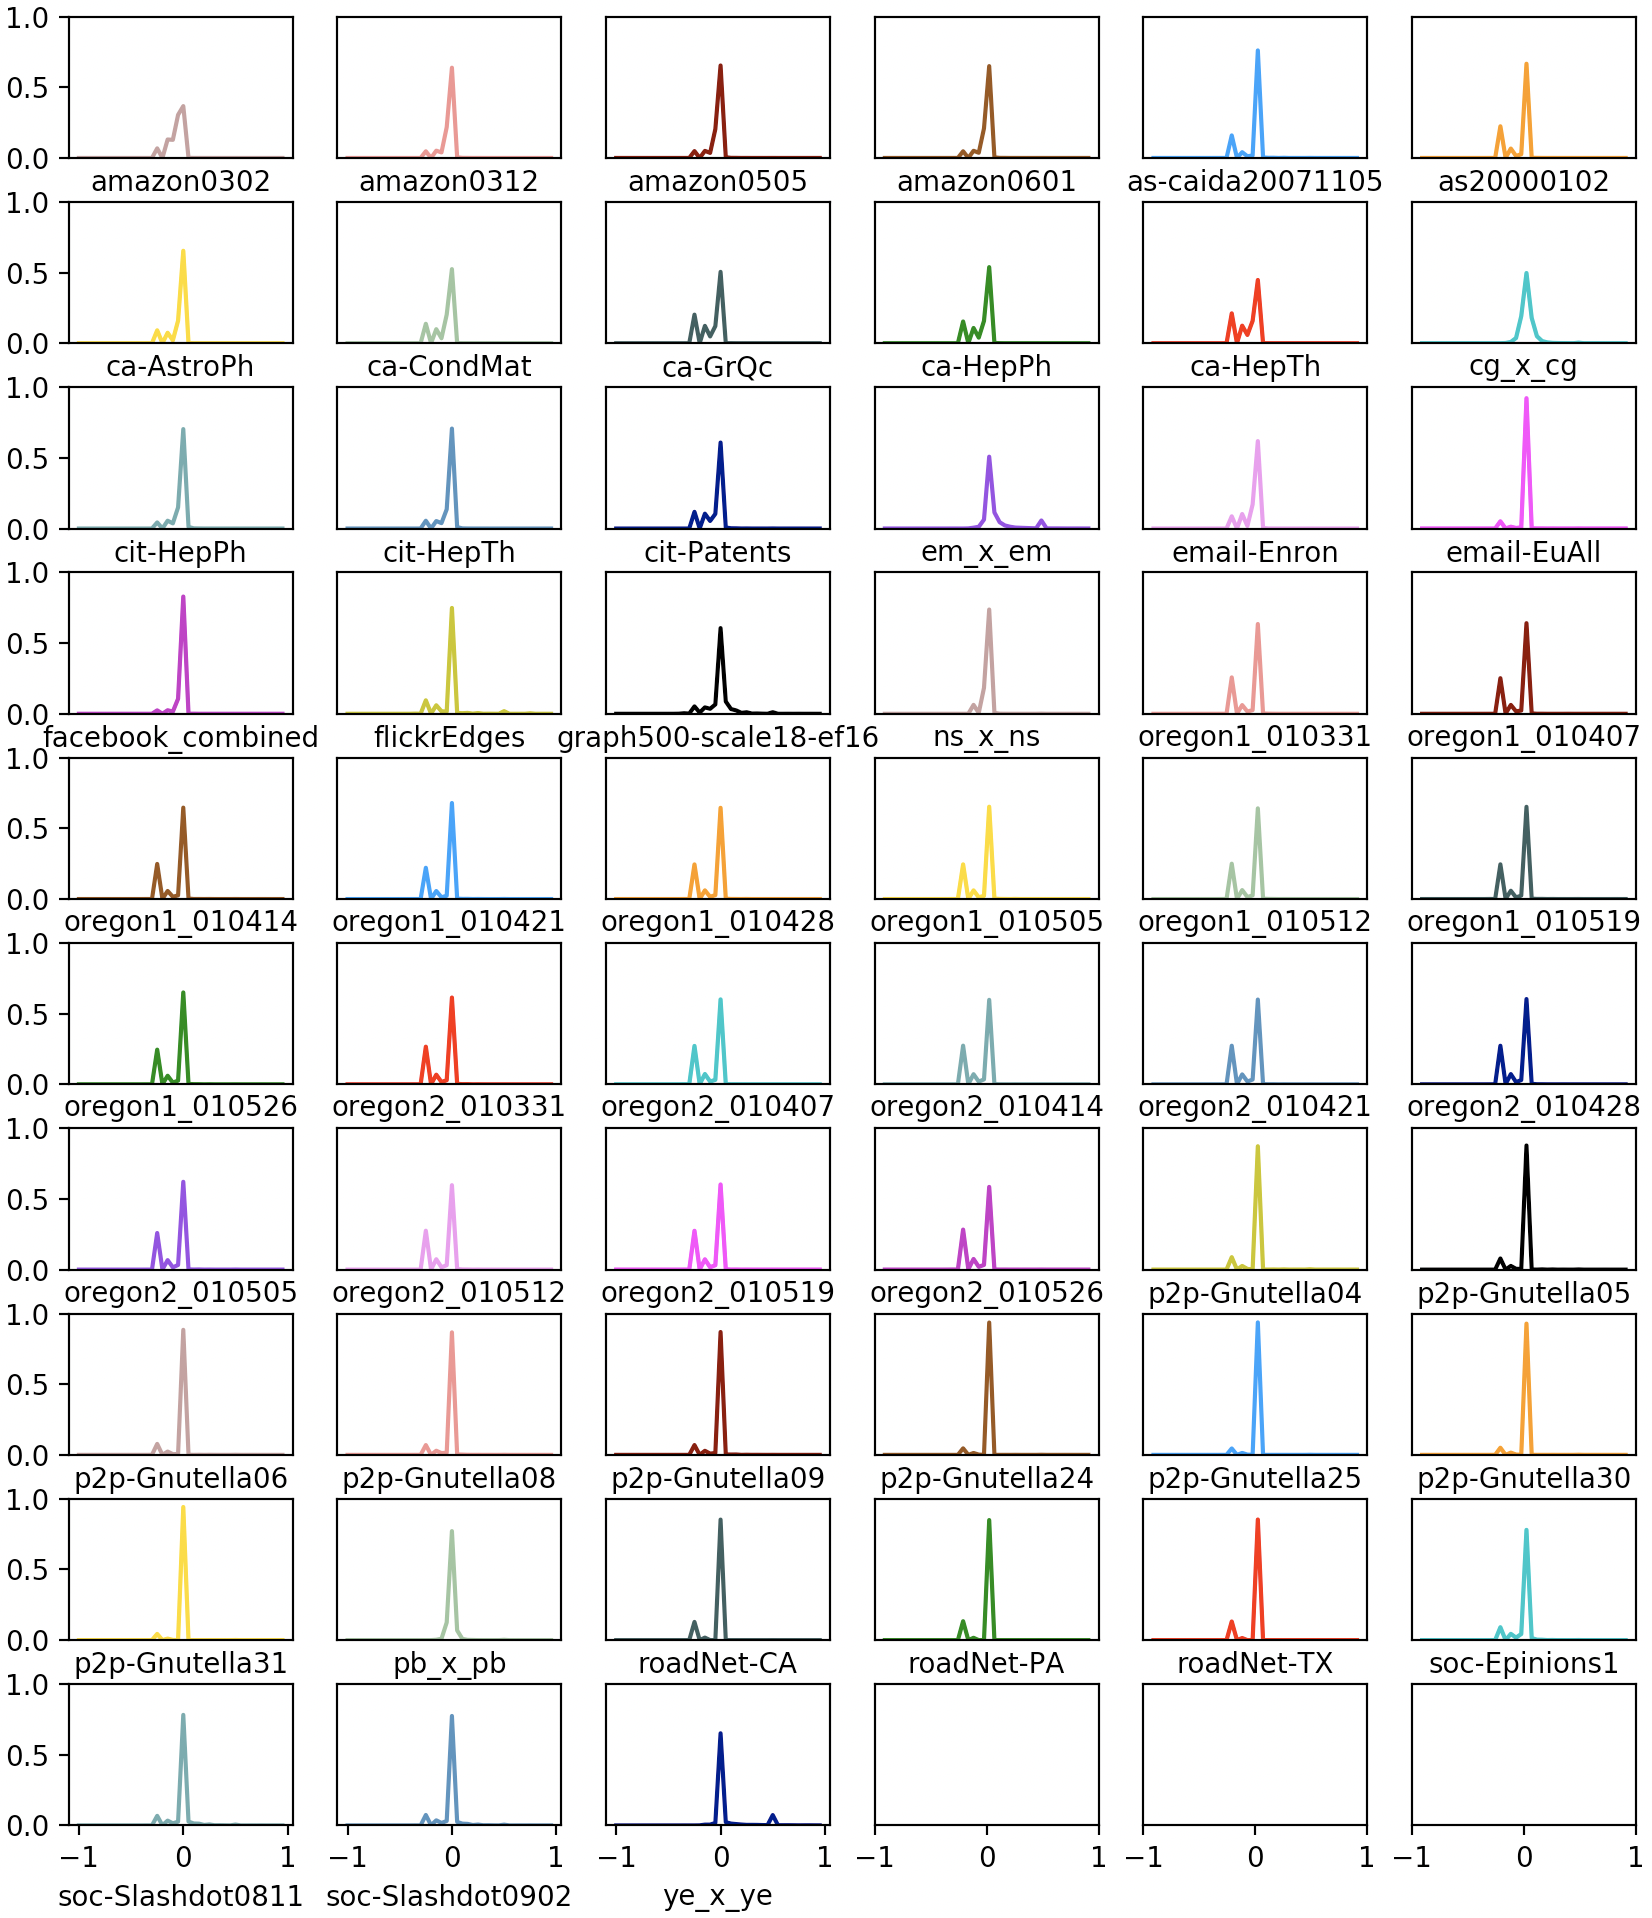
\includegraphics[width=1.0\columnwidth]{distn_vertex_total}}
	\caption{The vertex-local relative error of most of the  Table~\ref{tab:scaling_graphs} using $p=12$.
	\label{fig:distn_vertex}}
\end{figure}



\begin{figure}
	\centerline{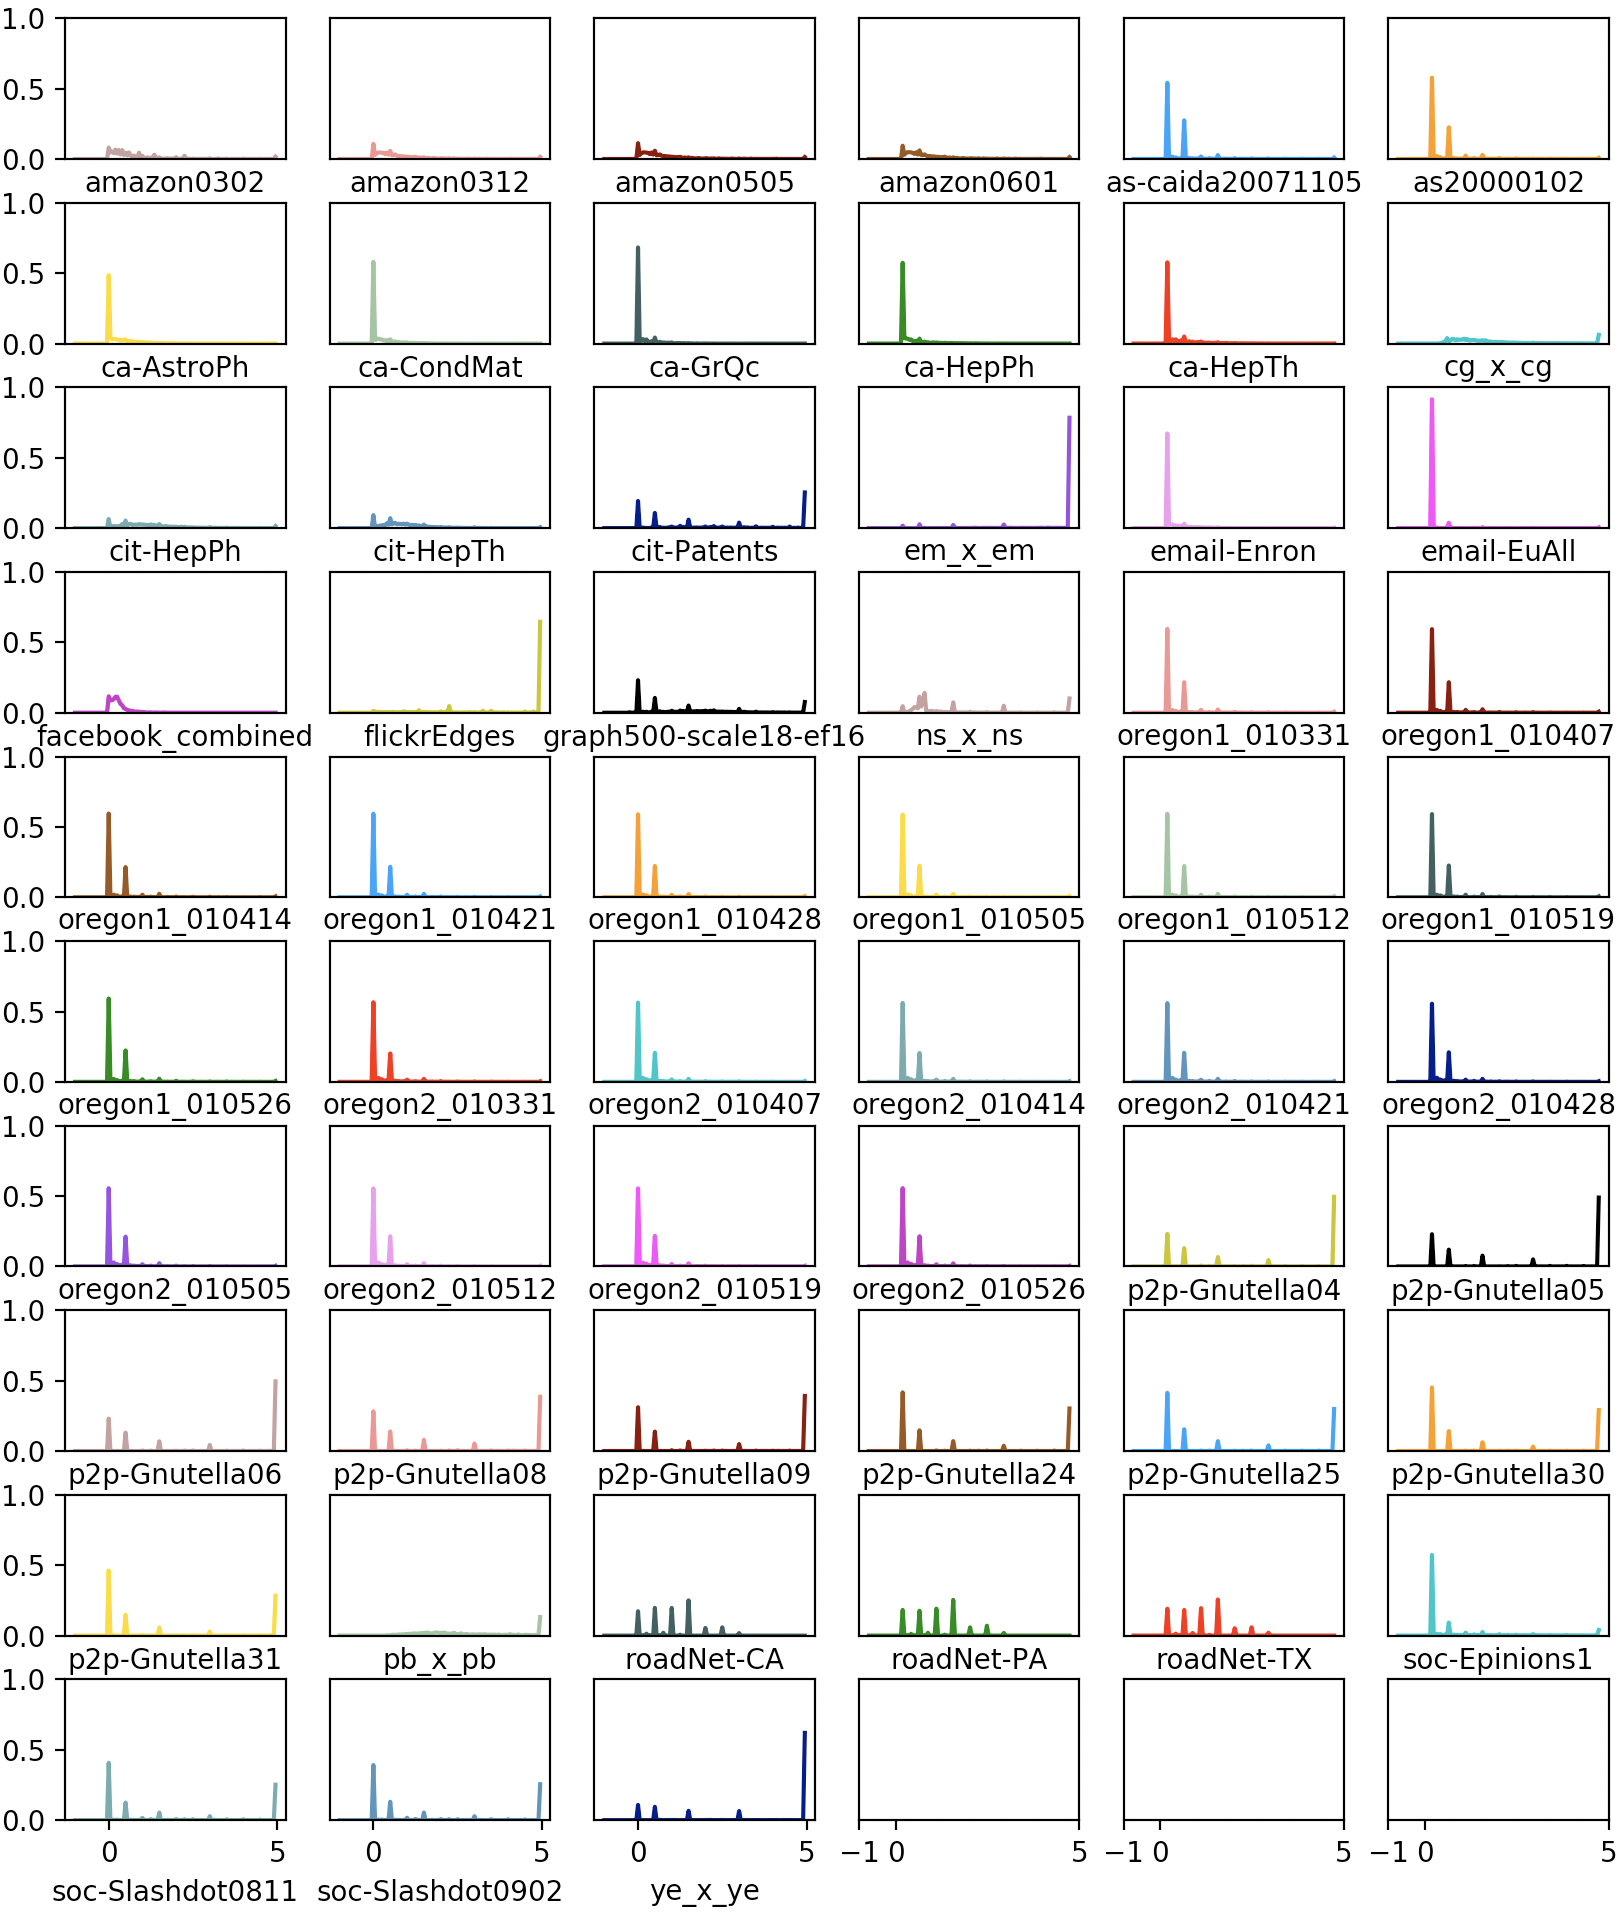
\includegraphics[width=1.0\columnwidth]{distn_naive_vertex_total}}
	\caption{The edge-local relative error of most of the  Table~\ref{tab:scaling_graphs} using $p=12$ and the na\"ive inclusion-exclusion intersection estimator. 
	Note that we have had to widen horizontal axis to account for large overestimates in graphs. 
	Note the degraded performance compared to Figure~\ref{fig:distn_vertex}.
	\label{fig:distn_naive_vertex}}
\end{figure}


Figure~\ref{fig:distn_vertex} plots the distributions of vertex local signed errors for the graphs using the maximum likelihood estimator. 
We should expect worse performance for vertex local triangle count estimation, as the estimates are composed of many triangle count estimates.
Indeed, we find that the experimental results no longer appear unbiased, as many vertices appear to underestimate their true triangle counts in most graphs. 
Compare these results with those of the na\"ive inclusion-exclusion estimator in Figure~\ref{fig:distn_naive_vertex}.
Similar to Figure~\ref{fig:distn_naive_edge}, we have widened the horizontal axis and some plots exhibit spikes at 5.
Figure~\ref{fig:distn_naive_vertex} tells a similar story to Figure~\ref{fig:distn_naive_edge}, with large overestimates in a large proportion of the vertex population.
Again, we find that the MLE estimator is much more reliable.

\begin{figure}
	\centerline{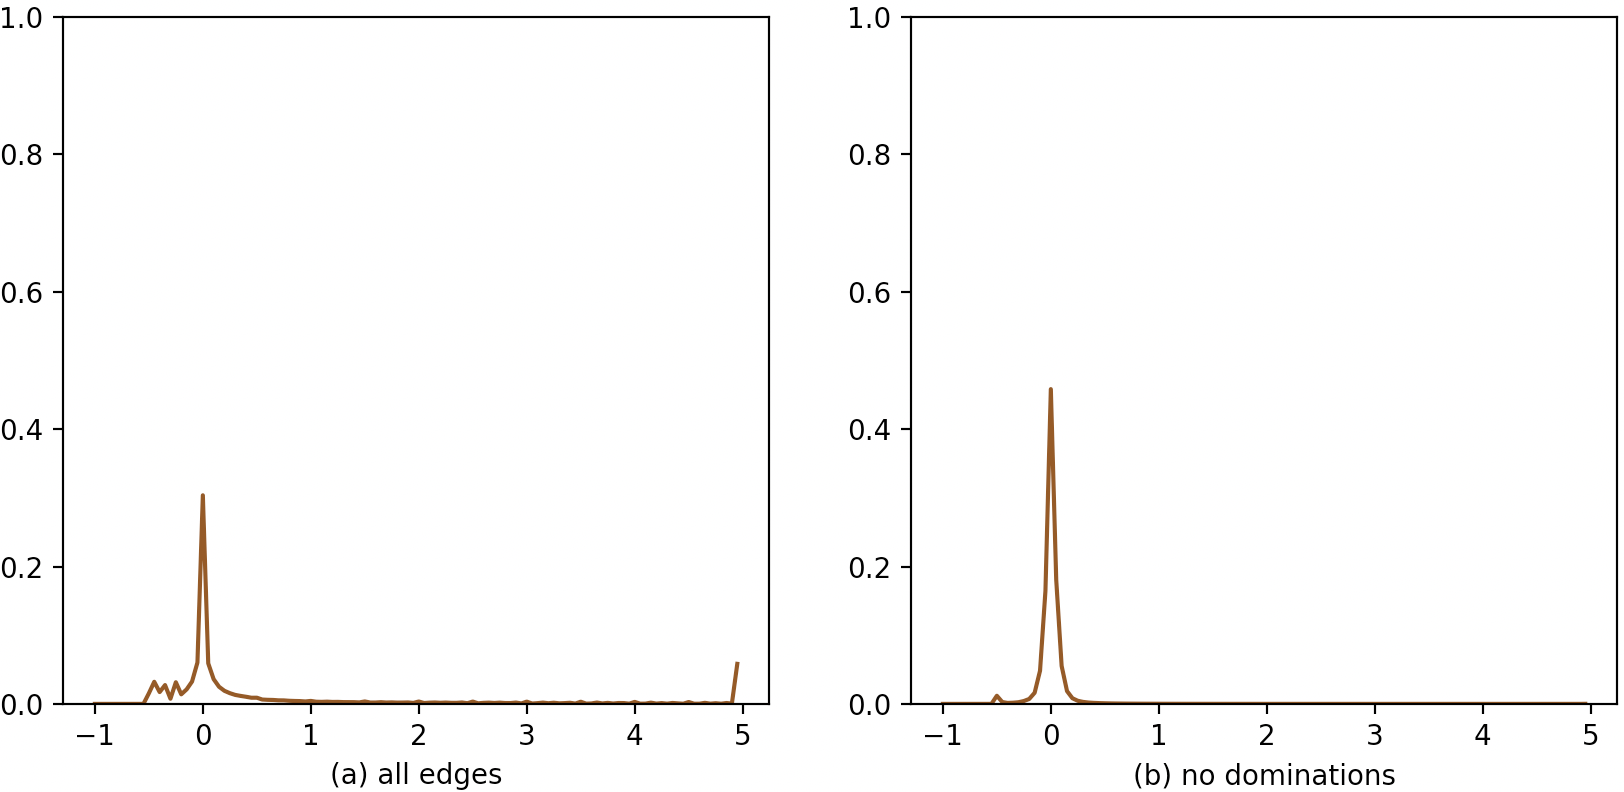
\includegraphics[width=0.8\columnwidth]{dist_twitter}}
	\caption{The edge local relative error distribution of the twitter graph (see Table~\ref{tab:scaling_graphs}).
	The distribution over all intersections (a) displays the heavy tail of overestimates.
	The distribution over only intersections not involving a domination (b) does not exhibit this tail, indicating that minimizing dominations results in improved relative error performance.
	\label{fig:dist_twitter}}
\end{figure}


We should be careful about generalizing these results to truly massive graphs, however.
As we noted in Section~\ref{DS:sec:experiments:intersection}, maintaining a constant bound on dominations is dependent upon graph size. 
That is, for fixed $p$, there will be a point as we increase the size of scale-free graphs where the error distribution will cease to look like the better examples in Figure~\ref{fig:distn_edge}. 
For example, consider Figure~\ref{fig:dist_twitter}, which plots the edge local signed error distributions for the larger Twitter graph (see Table~\ref{tab:scaling_graphs}).
This plot shows that the larger twitter graph involves a large number of dominations, which result in a heavy tail in the error distribution. 
When dominations are discounted, however, the result is a much more well behaved distribution.
While maintaining a low proportion of dominations is key, as we have established the only way to do so in the presence of increasing set size is to increase $p$.
Thus, in order to scale to immense graphs sketch size must increase as well, which is an undesirable feature. 

\begin{figure}
	\begin{center}
		\begin{subfigure}{0.32\linewidth}
			\centerline{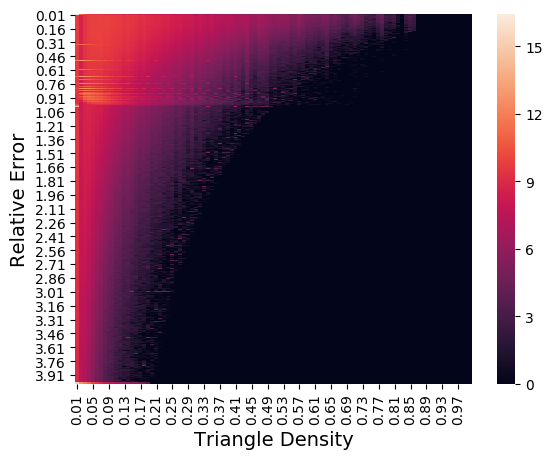
\includegraphics[width=1.0\columnwidth]{em_x_em_edge_dist_p8}}
			\caption{em $\otimes$ em, $p=8$. \label{fig:em_x_em_edge_density_vs_rel_err_p8}}
		\end{subfigure}
		\begin{subfigure}{0.32\linewidth}
			\centerline{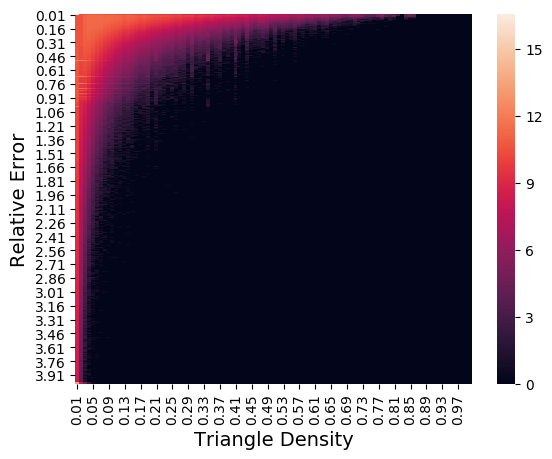
\includegraphics[width=1.0\columnwidth]{em_x_em_edge_dist_p12}}
			\caption{em $\otimes$ em, $p=12$. \label{fig:em_x_em_edge_density_vs_rel_err_p12}}
		\end{subfigure}
		\begin{subfigure}{0.32\linewidth}
			\centerline{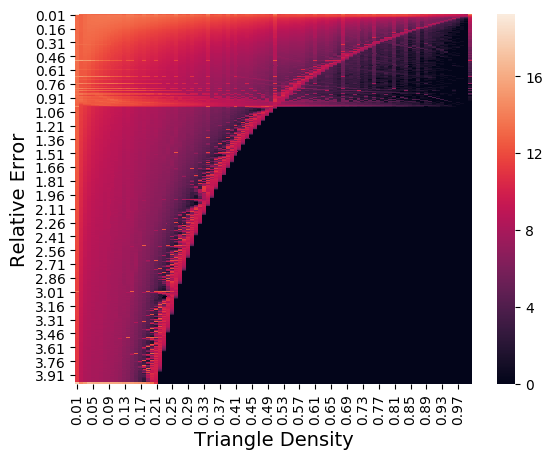
\includegraphics[width=1.0\columnwidth]{twitter_edge_dist_p12}}
			\caption{Twitter, $p=12$. \label{fig:twitter_edge_density_vs_rel_err_p12}}
		\end{subfigure}
		\caption{Heat maps displaying the distribution of edge-local triangle count relative error versus triangle density for the em $\otimes$ em and Twitter graphs. 
			Heat values asigned to cells are the logarithm of the number of edges matching that triangle density and relative error.
		 	Note that performance drastically improves for the em $\otimes$ em graph when $p$ increases from 8 to 12.
			\label{fig:edge_density_vs_rel_err}}
	\end{center}
\end{figure}

Consider also Figure~\ref{fig:edge_density_vs_rel_err}. 
This figure plots the distribution of observed relative errors versus triangle density for the em $\otimes$ em graph and the same Twitter graph explored in Figure~\ref{fig:dist_twitter}.
Note that the twitter graph is about two orders of magnitude larger than the em $\otimes$ em graph. 
We see a marked improvement in the distribution of error for the em $\otimes$ em graph as $p$ increases. 
While $p=12$ is clearly sufficient for the em $\otimes$ em graph, scaling to the Twitter graph clearly requires larger $p$.




\subsubsection{MLE performance statistics}

Table~\ref{tab:mle_performance} examines the maximum likelihood estimator performance on the graph in Table~\ref{tab:graphs} in specific detail. 
Note that these are the data from only a single run of the algorithm on each graph, as this is sufficient information to glean the distribution of errors on edge and vertex local estimates because each operation is performed a large number of times in each experiment.
The table plots the global relative error Eq.~\eqref{eq:global_error}, the number of dominations, the edge mean relative error Eq.~\eqref{eq:edge_mre}, the edge variance, the edge Vigna's $\tau_{h, \phi_{100}}$, the vertex mean relative error Eq.~\eqref{eq:vertex_mre}, the vertex variance, and the vertex Vigna's $\tau_{h, \phi_{100}}$.
The Vigna's $\tau_{h, \phi_{100}}$ statistics provide a quantificaton of the heavy hitter recovery performance similar to the precision versus recall, where elements at the very top of the ground truth triangle count are weighted more heavily than those near $100$.
It also serves as a better general purpose statistic. 

\begin{table}
\caption{MLE performance on all graphs, including global MRE, \# dominations, MRE and variance and $\tau_{h, \phi_{100}}$ for edges and vertices. \label{tab:mle_performance}}
\resizebox{\textwidth}{!}{
\begin{tabular}{|c|c|c|c|c|c|c|c|c|}
\hline
&  & & \multicolumn{3}{c}{edges} & \multicolumn{3}{c}{vertices} \\
\textbf{graph name} & global MRE & \# doms & MRE & variance & $\tau_{h, \phi_{100}}$ &  MRE & variance & $\tau_{h, \phi_{100}}$ \\
\hline
\hline
amazon0302&0.000410871 & 37258 & 0.00511415 & 0.00236737 & 0.948169 & 0.00617304 & 0.00174465 & 0.862339 \\
\hline
amazon0312&0.00101454 & 97923 & 0.0147273 & 0.0066181 & 0.969474 & 0.0109858 & 0.00210728 & 0.910493 \\
\hline
amazon0505&0.0045002 & 105156 & 0.0157157 & 0.00815814 & 0.971034 & 0.011564 & 0.00238126 & 0.9086 \\
\hline
amazon0601&0.000363835 & 101666 & 0.0147765 & 0.00686827 & 0.971244 & 0.0110941 & 0.00214676 & 0.90911 \\
\hline
as-caida20071105&0.0329567 & 1848 & 0.0592927 & 0.0292914 & 0.854042 & 0.0394628 & 0.0159984 & 0.765845 \\
\hline
as20000102&0.0321906 & 425 & 0.040091 & 0.0139573 & 0.694214 & 0.0271399 & 0.00551577 & 0.764055 \\
\hline
ca-AstroPh&0.0020574 & 8326 & 0.0183591 & 0.00194955 & 0.915358 & 0.00705243 & 0.0014227 & 0.678024 \\
\hline
ca-CondMat&0.00014373 & 3740 & 0.00790223 & 0.00135315 & 0.870845 & 0.00701574 & 0.00271152 & 0.720792 \\
\hline
ca-GrQc&0.00554309 & 500 & 0.00440433 & 0.000970238 & 0.506617 & 0.00647719 & 0.00275309 & 0.678824 \\
\hline
ca-HepPh&0.00248209 & 4927 & 0.0107195 & 0.00133045 & 0.899939 & 0.00842168 & 0.00227844 & 0.684348 \\
\hline
ca-HepTh&0.00359288 & 1112 & 0.00499942 & 0.00117584 & 0.788572 & 0.00820159 & 0.0037099 & 0.771194 \\
\hline
\textbf{cg $\boldsymbol{\otimes}$ cg}&0.00450143 & 80556 & 0.180783 & 0.059384 & 0.979046 & 0.115359 & 1.10753 & 0.0957111 \\
\hline
cit-HepPh&0.000491567 & 17143 & 0.0383193 & 0.00859173 & 0.930214 & 0.0150293 & 0.00176638 & 0.717774 \\
\hline
cit-HepTh&3.17927e-05 & 16412 & 0.0389419 & 0.00744493 & 0.929648 & 0.0137159 & 0.00178527 & 0.764128 \\
\hline
cit-Patents&0.00780909 & 692085 & 0.0238169 & 0.0134303 & 0.98958 & 0.0183164 & 0.0102654 & 0.97152 \\
\hline
\textbf{em $\boldsymbol{\otimes}$ em}&0.0269762 & 618030 & 0.361598 & 0.694572 & 0.970543 & 1.39935 & 29.4262 & 0.935464 \\
\hline
email-Enron&0.00237792 & 8728 & 0.0308221 & 0.00570846 & 0.904239 & 0.0125266 & 0.00314965 & 0.791837 \\
\hline
email-EuAll&0.0071636 & 10901 & 0.0438659 & 0.0250123 & 0.925389 & 0.00995284 & 0.00762299 & 0.91131 \\
\hline
facebook\_combined&0.00280804 & 3362 & 0.0115543 & 0.000545316 & 0.834189 & 0.00737009 & 0.000233799 & 0.536985 \\
\hline
flickrEdges&0.00341508 & 102572 & 0.0471881 & 0.0218786 & 0.983674 & 0.195658 & 32.6787 & 0.730175 \\
\hline
graph500-scale18-ef16&0.0165722 & 160923 & 0.138074 & 0.0367471 & 0.977851 & 0.133161 & 0.0554794 & 0.230933 \\
\hline
\textbf{ns $\boldsymbol{\otimes}$ ns}&0.000667794 & 155908 & 0.0160818 & 0.00657722 & 0.953689 & 0.0199951 & 0.0686846 & 0.90299 \\
\hline
oregon1\_010331&0.0120226 & 973 & 0.0374072 & 0.0105397 & 0.81614 & 0.0283393 & 0.00623208 & 0.761701 \\
\hline
oregon1\_010407&0.00341295 & 923 & 0.0392721 & 0.0110109 & 0.800534 & 0.0297942 & 0.00548587 & 0.736287 \\
\hline
oregon1\_010414&0.0394825 & 1577 & 0.0413332 & 0.0159812 & 0.82125 & 0.0302528 & 0.00780099 & 0.751239 \\
\hline
oregon1\_010421&0.0119283 & 725 & 0.0397194 & 0.0180728 & 0.800203 & 0.0284574 & 0.00844028 & 0.758715 \\
\hline
oregon1\_010428&0.0178996 & 500 & 0.0450234 & 0.0149815 & 0.810885 & 0.0323162 & 0.00681453 & 0.733992 \\
\hline
oregon1\_010505&0.00514401 & 635 & 0.0374775 & 0.0133416 & 0.815531 & 0.0262984 & 0.00580777 & 0.764276 \\
\hline
oregon1\_010512&0.00372097 & 1369 & 0.0363218 & 0.0100373 & 0.812308 & 0.0266561 & 0.00477533 & 0.787779 \\
\hline
oregon1\_010519&0.00167728 & 839 & 0.0544582 & 0.0216188 & 0.805998 & 0.040216 & 0.0112947 & 0.756786 \\
\hline
oregon1\_010526&0.0257453 & 779 & 0.0394423 & 0.0163412 & 0.790612 & 0.0278942 & 0.00708625 & 0.77016 \\
\hline
oregon2\_010331&0.00215726 & 1065 & 0.0313933 & 0.0110602 & 0.814389 & 0.0265301 & 0.00632335 & 0.732991 \\
\hline
oregon2\_010407&0.0102734 & 1798 & 0.0399965 & 0.0124726 & 0.812382 & 0.0374412 & 0.0079474 & 0.764744 \\
\hline
oregon2\_010414&0.00214211 & 1139 & 0.0348277 & 0.00999769 & 0.828402 & 0.0317464 & 0.00610695 & 0.741403 \\
\hline
oregon2\_010421&0.00696287 & 1697 & 0.0349412 & 0.0116954 & 0.807914 & 0.0297692 & 0.00620846 & 0.763229 \\
\hline
oregon2\_010428&0.000930958 & 1518 & 0.0378781 & 0.0110547 & 0.829194 & 0.0321114 & 0.00601949 & 0.775626 \\
\hline
oregon2\_010505&0.00920473 & 1016 & 0.0361535 & 0.0133905 & 0.82981 & 0.0288103 & 0.00774782 & 0.78395 \\
\hline
oregon2\_010512&0.000384439 & 1312 & 0.0425334 & 0.0146203 & 0.801557 & 0.0366068 & 0.00780288 & 0.787347 \\
\hline
oregon2\_010519&0.00208633 & 1194 & 0.0378019 & 0.0107673 & 0.839299 & 0.0333108 & 0.00662257 & 0.754128 \\
\hline
oregon2\_010526&0.00106532 & 1473 & 0.0514426 & 0.0174551 & 0.835291 & 0.0515479 & 0.0123812 & 0.769886 \\
\hline
p2p-Gnutella04&0.148558 & 1555 & 0.0177248 & 0.0168244 & 0.695298 & 0.0489285 & 0.111457 & 0.762134 \\
\hline
p2p-Gnutella05&0.121239 & 1310 & 0.0151124 & 0.0137138 & 0.808389 & 0.034442 & 0.0241619 & 0.728775 \\
\hline
p2p-Gnutella06&0.063464 & 1191 & 0.0146142 & 0.0124697 & 0.802282 & 0.0345433 & 0.0267341 & 0.66756 \\
\hline
p2p-Gnutella08&0.0728463 & 754 & 0.0174324 & 0.0119514 & 0.752416 & 0.0241876 & 0.0191441 & 0.6 \\
\hline
p2p-Gnutella09&0.135828 & 1110 & 0.0200961 & 0.0146221 & 0.804122 & 0.0272512 & 0.0165108 & 0.6878 \\
\hline
p2p-Gnutella24&0.219074 & 2730 & 0.0109942 & 0.0103753 & 0.819203 & 0.0219898 & 0.0254313 & 0.859488 \\
\hline
p2p-Gnutella25&0.291334 & 2322 & 0.00901289 & 0.00842632 & 0.758603 & 0.0191121 & 0.0239306 & 0.820848 \\
\hline
p2p-Gnutella30&0.173799 & 3829 & 0.0107415 & 0.0101481 & 0.851817 & 0.0216437 & 0.0322464 & 0.808806 \\
\hline
p2p-Gnutella31&0.228864 & 6211 & 0.0102196 & 0.00964274 & 0.886073 & 0.0204559 & 0.020475 & 0.767571 \\
\hline
\textbf{pb $\boldsymbol{\otimes}$ pb}&0.0142477 & 4671 & 0.0801485 & 0.0248473 & 0.858059 & 0.0969235 & 0.6582 & 0.569607 \\
\hline
roadNet-CA&0.0059839 & 113001 & 0.000806493 & 0.000731067 & 0.567993 & 0.00130683 & 0.00097556 & 0.985063 \\
\hline
roadNet-PA&0.00545083 & 63207 & 0.000781687 & 0.000702402 & 0.590963 & 0.00126972 & 0.000967292 & 0.99904 \\
\hline
roadNet-TX&0.0053398 & 78363 & 0.000763467 & 0.000690403 & 0.579244 & 0.00126706 & 0.000940359 & 1.0 \\
\hline
soc-Epinions1&0.0041685 & 19872 & 0.0823205 & 0.025062 & 0.927086 & 0.0256688 & 0.0086639 & 0.841355 \\
\hline
soc-Slashdot0811&0.0219384 & 19301 & 0.152505 & 0.0902361 & 0.937038 & 0.0713931 & 0.044451 & 0.855897 \\
\hline
soc-Slashdot0902&0.0153844 & 20220 & 0.145098 & 0.0816233 & 0.949649 & 0.0664616 & 0.0370551 & 0.890315 \\
\hline
\textbf{ye $\boldsymbol{\otimes}$ ye}&0.128437 & 926066 & 0.381506 & 0.930024 & 0.991193 & 2.15683 & 110.979 & 0.943107 \\
\hline
\end{tabular}}
\end{table}

The results in Table~\ref{tab:mle_performance} indicate that our algorithms produce surprisingly good estimates on all edges and vertices, not just heavy hitters, for sufficiently large $p$. 
Note that the worst performers in terms of mean relative error are the large synthetic Kronecker graphs $em \otimes em$ and $ye \otimes ye$, which also experience a large volume of dominations. 
Increasing $p$, of course, improves performance on these graphs at the expense of increased memory, communication, and computation overhead. 




%}
%----------------------------------------------------------------------------------------
\subsubsection{Scaling to Massive Graphs}
%----------------------------------------------------------------------------------------

We have already discussed the challenges in scaling intersections to large graphs. 
We will now examine the performance scaling of the algorithms as a function of data and computing resource sizes.
An advantage of this analysis is that it extends to other applications of \algoname{DegreeSketch}, such as the distributed neighborhood estimation algorithm discussed in Section~\ref{DS:sec:neighborhoods}.

\begin{table}[htbp]
\caption{Scaling Graphs \label{tab:scaling_graphs}}
\begin{center}
\begin{tabular}{|c|c|c|c|}
\hline
\textbf{graph} & $|\mathcal{V}|$ &  $|\mathcal{E}|$ & Type \\
\hline
\hline
patents & 3,774,768 & 16,518,947 & Citation \\
\hline
\textbf{ye $\boldsymbol{\otimes}$ ye} & 5,574,320 & 88,338,632 & Kronecker \\
\hline
\textbf{or $\boldsymbol{\otimes}$ or} & 131,859,288 & 1,095,962,562 & Kronecker \\
\hline
Twitter & 41,652,224 & 1,201,045,942 & Soc. Net. \cite{kunegis2013konect} \\
\hline
WebDataCommons & 3,563,602,788 & 128,736,914,864 & Web \\
\hline
\end{tabular}
\end{center}
\end{table}


For our scaling experiments we ran Algorithm~\ref{alg:ds:accumulation} (accumulation) and Algorithm~\ref{alg:ds:vertex_local} (vertex local estimation) on each graph in Table~\ref{tab:scaling_graphs}.
Note that some of these graphs are much larger than those considered in Table~\ref{tab:graphs}.
We used $p=8$ for efficacy, as we are interested in scaling and not concerned with the estimation quality in this case. 
We discounted the I/O time spent on reading data streams from files.

It is worth noting that a competing state-of-the-art exact triangle counting algorithm required $N=256$ compute nodes to even load the largest WebDataCommons graph into distributed memory \cite{pearce2017triangle}.

\begin{figure}
	\centerline{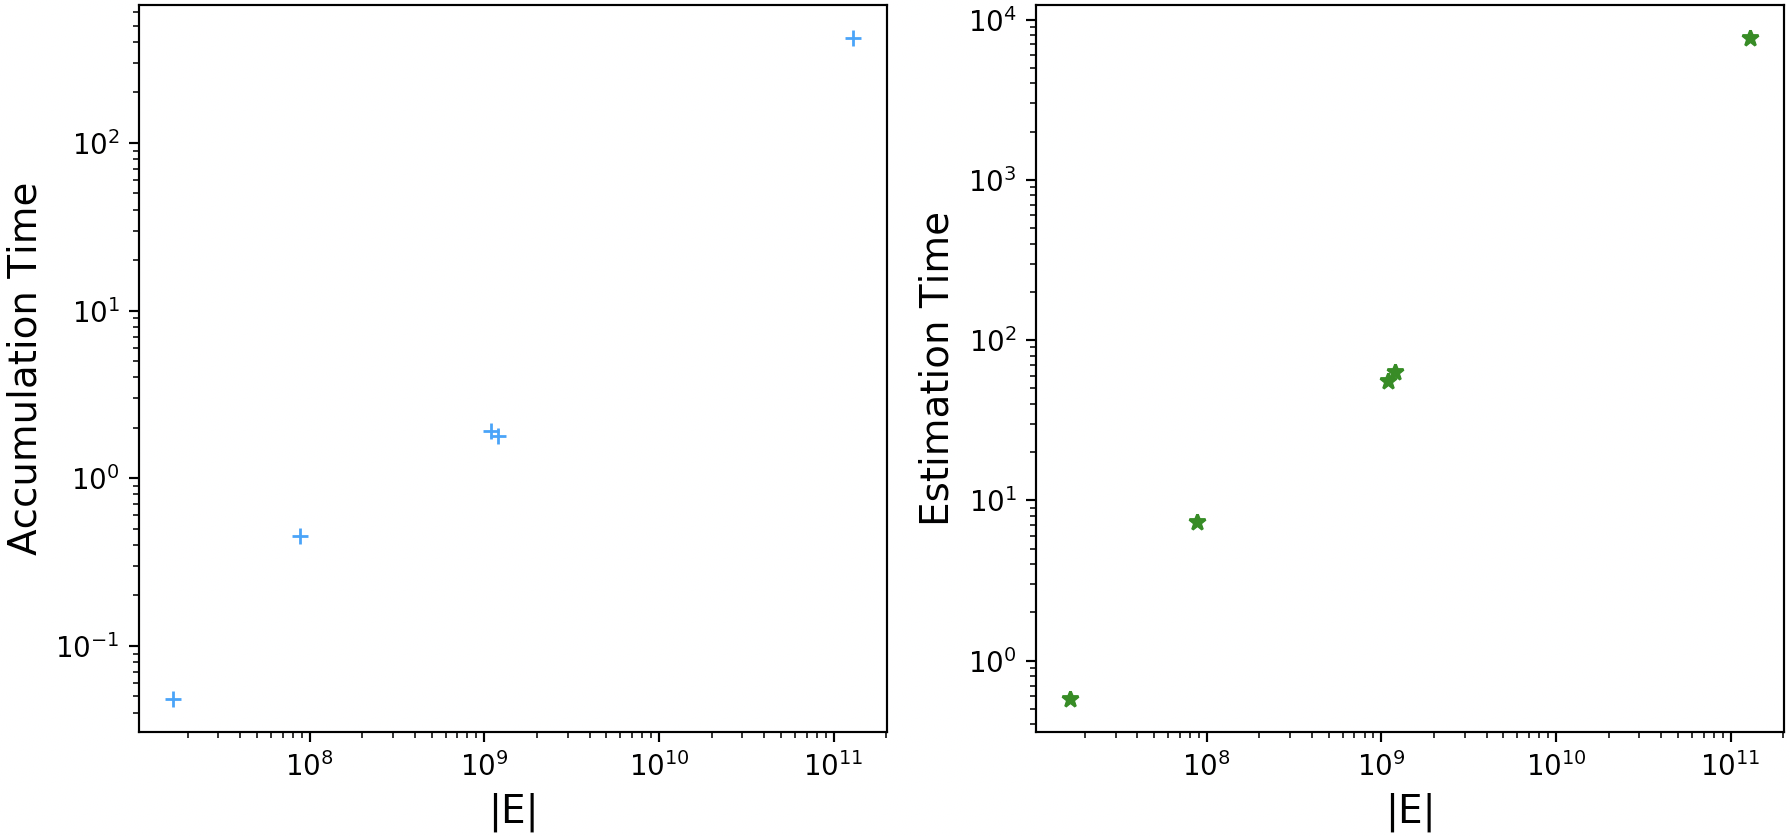
\includegraphics[width=0.8\columnwidth]{ds_scaling}}
	\caption{The time in seconds to accumulate and estimate using $N=72$ compute nodes, each of which have 24 cores, for all graphs listed in Table~\ref{tab:scaling_graphs} using $p=8$.
	We have ignored the time taken reading from streams and included only the time spend on local computations and communication.
	This shows that linear scaling in $|\mathcal{E}|$ extends out to truly massive graphs.
	\label{fig:ds_scaling}}
\end{figure}

\begin{figure}
	\centerline{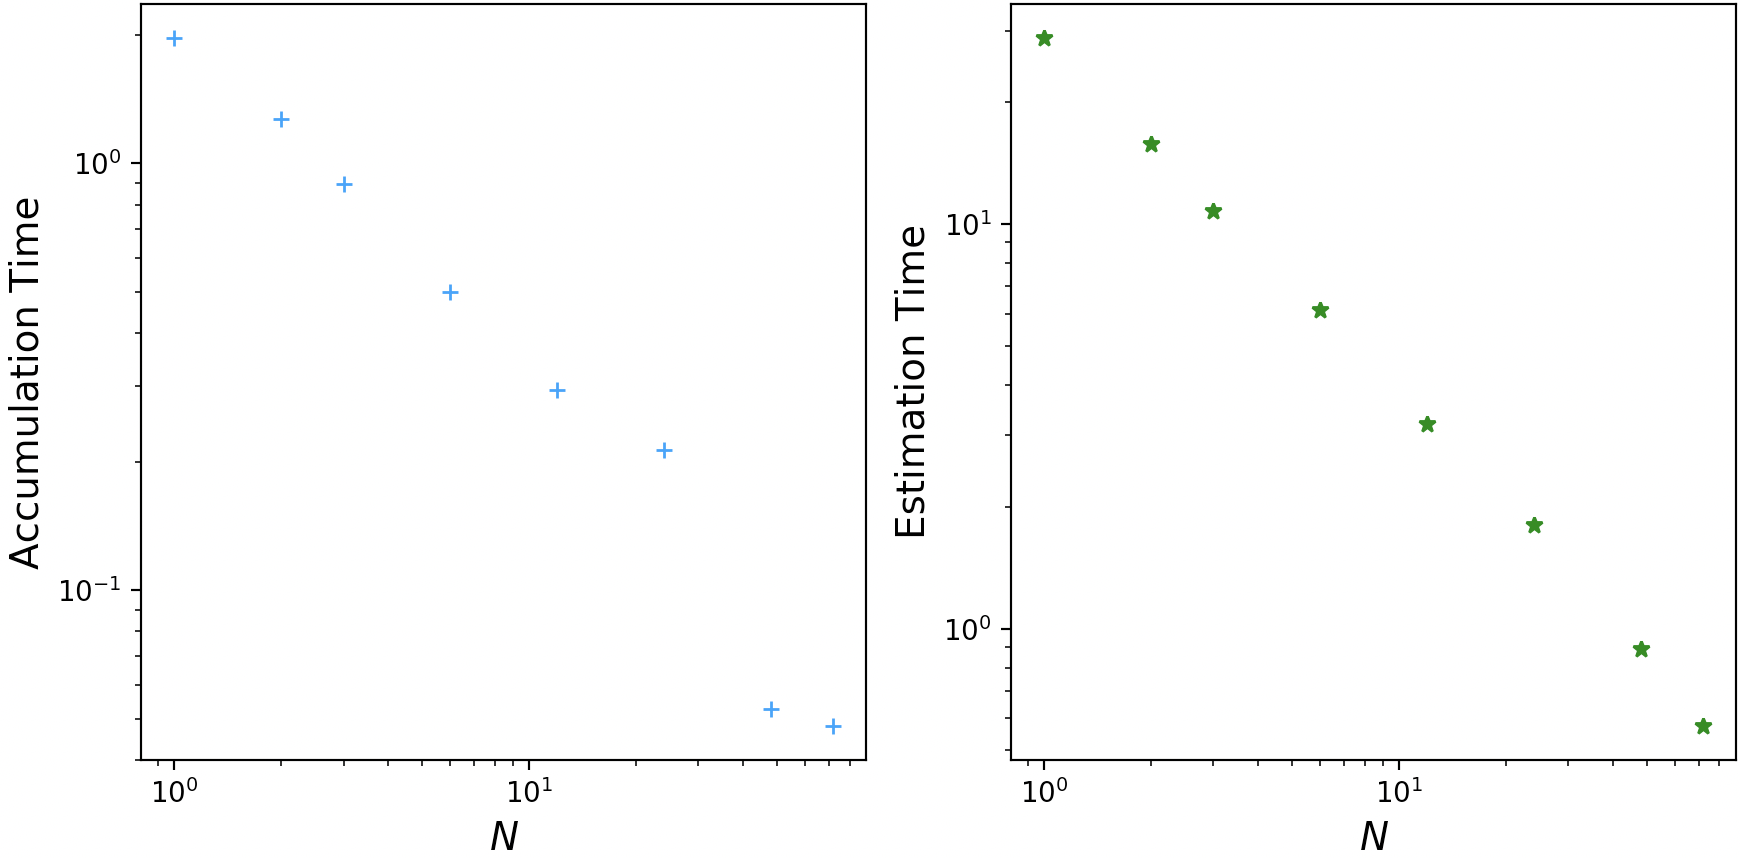
\includegraphics[width=0.8\columnwidth]{patents_scaling}}
	\caption{The time in seconds to accumulate and estimate using $N=1$ up to $72$ compute nodes, each of which have 24 cores, for the citation-Patents graph using $p=8$.
	We have ignored the time taken reading from streams and included only the time spend on local computations and communication.
	This shows inverse linear scaling as $N$ increases and the workload remains the same.
	\label{fig:patents_scaling}}
\end{figure}

Figure~\ref{fig:ds_scaling} measures the the time in seconds spent accumulating $\algoname{DegreeSketch}$ and performing the vertex-local estimation on each graph, plotted against the number of edges in each graph. 
We used $N=72$ compute nodes in each case. 
As promised, the wall time is linear in the number edges for both accumulation and estimation.
Similarly, Figure~\ref{fig:patents_scaling} measures the the time in seconds spent accumulating $\algoname{DegreeSketch}$ and performing the vertex-local estimation on the cit-Patents graph, where $N$ varies from 1 up to 72. 
The wall time gain of increasing $N$ is linear in this case as well. 



%\begin{figure}
%	\begin{center}
%		\begin{subfigure}{0.49\linewidth}
%			\centerline{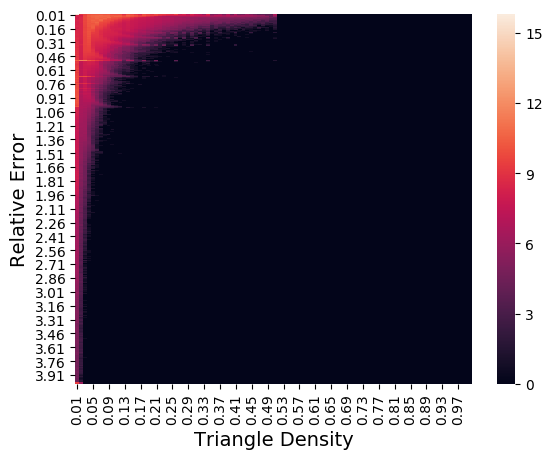
\includegraphics[width=1.0\columnwidth]{patents_edge_distn_density_vs_rel_err.png}}
%			\caption{cit-Patents. \label{fig:patents_edge_density_vs_rel_err}}
%		\end{subfigure}
%		\begin{subfigure}{0.49\linewidth}
%			\centerline{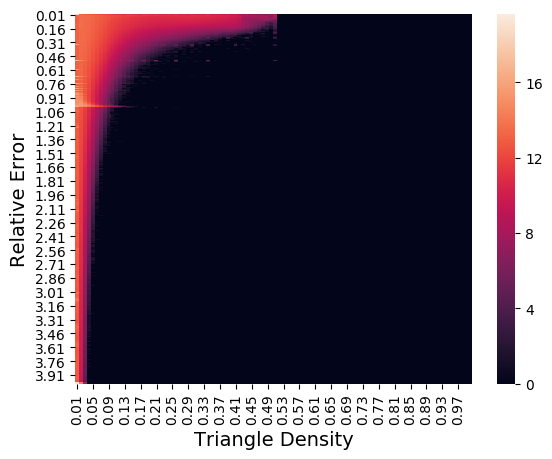
\includegraphics[width=1.0\columnwidth]{twitter_edge_distn_density_vs_rel_err.png}}
%			\caption{Twitter. \label{fig:twitter_edge_density_vs_rel_err}}
%		\end{subfigure}
%		\caption{Heat maps displaying the distribution of edge-local triangle count relative error for two large graphs where $p = 12$.
%			Heat values asigned to cells are the logarithm of the number of edges matching that triangle density and relative error.
%			\label{fig:edge_density_vs_rel_err}}
%	\end{center}
%\end{figure}

%\begin{table}[htbp]
%\caption{Graph Scaling \label{tab:graphs}}
%\begin{center}
%\begin{tabular}{|c|c|c|c|c|c|}
%\hline
%\textbf{graph} & $|\mathcal{V}|$ &  $|\mathcal{E}|$ & $|\mathcal{T}|$ & Type \\
%\hline
%\hline
%patents & 3,774,768 & 16,518,947   & 7,515,020& Citation \\
%\hline
%\textbf{ye $\boldsymbol{\otimes}$ ye} & 5,574,320 & 88,338,632 & 74,765,400 & Kronecker \\
%\hline
%\textbf{or $\boldsymbol{\otimes}$ or} & 131,859,288 & 1,095,962,562 & 7,123,882,248 & Kronecker \\
%\hline
%Twitter & 41,652,224 & 1,201,045,942 &  104,079,430,149 & Soc. Net. \cite{konect2016twitter} \\
%\hline
%WebData & 3,563,602,788 & 128,736,914,864 &  \#\#\# & Web \\
%\hline
%\end{tabular}
%\end{center}
%\end{table}



%\begin{longtable}{|c|c|c|c|c|c|c|c|}
%\hline
%\textbf{graph} & $|E|$ & $|T|$ & $\frac{|T|}{|E|}$ & $\frac{||T| - |\tilde{T}||}{|T|}$ & top 10 MRE & top 100 MRE & top 1000 MRE \\
%\hline
%as20000102 & 12572 & 6584 & 0.52 & 3.2815 & 0.0781 & 0.1719 & 0.4974 \\
%\hline
%ca-GrQc & 14484 & 48260 & 3.33 & 0.0072 & 0.0125 & 0.0133 & 0.0127 \\
%\hline
%p2p-Gnutella08 & 20777 & 2383 & 0.11 & 0.0923 & 0.0549 & 0.0932 & 0.2424 \\
%\hline
%oregon1010407 & 21999 & 15834 & 0.72 & 1.4523 & 0.0795 & 0.1244 & 0.3531 \\
%\hline
%oregon1010331 & 22002 & 17144 & 0.78 & 1.2731 & 0.1 & 0.121 & 0.2807 \\
%\hline
%oregon1010414 & 22469 & 18237 & 0.81 & 1.2338 & 0.0604 & 0.1147 & 0.3056 \\
%\hline
%oregon1010428 & 22493 & 17645 & 0.78 & 1.4769 & 0.0659 & 0.1234 & 0.3274 \\
%\hline
%oregon1010505 & 22607 & 17597 & 0.78 & 1.2909 & 0.0684 & 0.1258 & 0.3187 \\
%\hline
%oregon1010512 & 22677 & 17598 & 0.78 & 1.3222 & 0.0666 & 0.1202 & 0.3137 \\
%\hline
%oregon1010519 & 22724 & 17677 & 0.78 & 1.396 & 0.0643 & 0.1234 & 0.315 \\
%\hline
%oregon1010421 & 22747 & 19108 & 0.84 & 1.1561 & 0.0648 & 0.1087 & 0.2862 \\
%\hline
%oregon1010526 & 23409 & 19894 & 0.85 & 1.3068 & 0.0717 & 0.1178 & 0.2838 \\
%\hline
%ca-HepTh & 25973 & 28339 & 1.09 & 0.0058 & 0.0079 & 0.0074 & 0.007 \\
%\hline
%p2p-Gnutella09 & 26013 & 2354 & 0.09 & 0.1347 & 0.0626 & 0.094 & 0.2683 \\
%\hline
%oregon2010407 & 30855 & 78138 & 2.53 & 0.2687 & 0.0607 & 0.0606 & 0.0485 \\
%\hline
%oregon2010505 & 30943 & 72182 & 2.33 & 0.3038 & 0.0499 & 0.0607 & 0.057 \\
%\hline
%oregon2010331 & 31180 & 82856 & 2.66 & 0.264 & 0.0674 & 0.0584 & 0.0473 \\
%\hline
%oregon2010512 & 31303 & 72866 & 2.33 & 0.3406 & 0.0525 & 0.06 & 0.0563 \\
%\hline
%oregon2010428 & 31434 & 78000 & 2.48 & 0.2612 & 0.0529 & 0.0583 & 0.0567 \\
%\hline
%p2p-Gnutella06 & 31525 & 1142 & 0.04 & 0.1909 & 0.0296 & 0.114 & 0.2764 \\
%\hline
%oregon2010421 & 31538 & 82129 & 2.6 & 0.3039 & 0.0478 & 0.0583 & 0.0532 \\
%\hline
%oregon2010414 & 31761 & 88905 & 2.8 & 0.2745 & 0.0501 & 0.0585 & 0.0493 \\
%\hline
%p2p-Gnutella05 & 31839 & 1112 & 0.03 & 0.5652 & 0.0557 & 0.1493 & 0.2506 \\
%\hline
%oregon2010519 & 32287 & 83709 & 2.59 & 0.2927 & 0.0569 & 0.0535 & 0.0557 \\
%\hline
%oregon2010526 & 32730 & 89541 & 2.74 & 0.3163 & 0.0487 & 0.0488 & 0.0531 \\
%\hline
%p2p-Gnutella04 & 39994 & 934 & 0.02 & 0.1534 & 0.0676 & 0.0825 & 0.1849 \\
%\hline
%as-caida20071105 & 53381 & 36365 & 0.68 & 0.9618 & 0.1049 & 0.1176 & 0.2616 \\
%\hline
%p2p-Gnutella25 & 54705 & 806 & 0.01 & 0.1521 & 0.037 & 0.0642 & 0.1341 \\
%\hline
%p2p-Gnutella24 & 65369 & 986 & 0.02 & 0.4879 & 0.0272 & 0.3085 & 0.3786 \\
%\hline
%facebookcombined & 88234 & 1612010 & 18.27 & 0.0675 & 0.0311 & 0.0234 & 0.0142 \\
%\hline
%p2p-Gnutella30 & 88328 & 1590 & 0.02 & 0.0596 & 0.0506 & 0.0616 & 0.1286 \\
%\hline
%ca-CondMat & 93439 & 173361 & 1.86 & 0.0074 & 0.0183 & 0.0199 & 0.0268 \\
%\hline
%ca-HepPh & 118489 & 3358500 & 28.34 & 0.0101 & 0.0108 & 0.0119 & 0.0117 \\
%\hline
%p2p-Gnutella31 & 147892 & 2024 & 0.01 & 0.3307 & 0.0525 & 0.0603 & 0.1043 \\
%\hline
%email-Enron & 183831 & 727044 & 3.95 & 0.0454 & 0.0438 & 0.0597 & 0.078 \\
%\hline
%ca-AstroPh & 198050 & 1351440 & 6.82 & 0.0085 & 0.0169 & 0.024 & 0.0233 \\
%\hline
%loc-brightkiteedges & 214078 & 494728 & 2.31 & 0.2306 & 0.0426 & 0.0308 & 0.0241 \\
%\hline
%cit-HepTh & 352285 & 1478740 & 4.2 & 0.0476 & 0.0259 & 0.0543 & 0.0744 \\
%\hline
%email-EuAll & 364481 & 267313 & 0.73 & 1.4844 & 0.0223 & 0.0727 & 0.1487 \\
%\hline
%\textbf{pb $\boldsymbol{\otimes}$ pb} & 388962 & 1881600 & 4.84 & 0.0215 & 0.044 & 0.0482 & 0.0523 \\
%\hline
%soc-Epinions1 & 405740 & 1624480 & 4.0 & 1.8267 & 0.0702 & 0.074 & 0.0832 \\
%\hline
%cit-HepPh & 420877 & 1276870 & 3.03 & 0.0269 & 0.0213 & 0.0292 & 0.036 \\
%\hline
%soc-Slashdot0811 & 469180 & 551724 & 1.18 & 0.1829 & 0.0883 & 0.0447 & 0.0548 \\
%\hline
%soc-Slashdot0902 & 504230 & 602592 & 1.2 & 0.2646 & 0.0204 & 0.0415 & 0.0523 \\
%\hline
%amazon0302 & 899792 & 717719 & 0.8 & 0.139 & 0.0441 & 0.0523 & 0.0457 \\
%\hline
%loc-gowallaedges & 950327 & 2273140 & 2.39 & 0.3591 & 0.1708 & 0.1834 & 0.2103 \\
%\hline
%roadNet-PA & 1541898 & 67150 & 0.04 & 0.014 & 0.0034 & 0.0035 & 0.0036 \\
%\hline
%roadNet-TX & 1921660 & 82869 & 0.04 & 0.0048 & 0.0033 & 0.0031 & 0.0033 \\
%\hline
%flickrEdges & 2316948 & 107987000 & 46.61 & 0.0108 & 0.0126 & 0.0109 & 0.0138 \\
%\hline
%amazon0312 & 2349869 & 3686470 & 1.57 & 0.0948 & 0.057 & 0.0474 & 0.049 \\
%\hline
%amazon0505 & 2439437 & 3951060 & 1.62 & 0.158 & 0.0656 & 0.044 & 0.0508 \\
%\hline
%amazon0601 & 2443408 & 3986510 & 1.63 & 0.1734 & 0.0612 & 0.0459 & 0.051 \\
%\hline
%roadNet-CA & 2766607 & 120676 & 0.04 & 0.0062 & 0.0047 & 0.0054 & 0.0041 \\
%\hline
%graph500-scale18-ef16 & 3800348 & 82287300 & 21.65 & 3.7168 & 0.0516 & 0.0523 & 0.0742 \\
%\hline
%\textbf{cg $\boldsymbol{\otimes}$ cg} & 8201250 & 64707900 & 7.89 & 0.3832 & 0.031 & 0.064 & 0.1362 \\
%\hline
%\textbf{ns $\boldsymbol{\otimes}$ ns} & 15037128 & 85006200 & 5.65 & 0.0015 & 0.018 & 0.0155 & 0.0158 \\
%\hline
%cit-Patents & 16518947 & 7515020 & 0.45 & 0.0044 & 0.0105 & 0.0127 & 0.016 \\
%\hline
%\textbf{em $\boldsymbol{\otimes}$ em} & 59426802 & 171286000 & 2.88 & 0.0222 & 0.1093 & 0.0985 & 0.0953 \\
%\hline
%\textbf{ye $\boldsymbol{\otimes}$ ye} & 88338632 & 74765400 & 0.85 & 0.054 & 0.0516 & 0.0605 & 0.0636 \\
%\hline
%\caption{Edge-Local Aggregate Performance \label{tab:big}}
%\end{longtable}

%------------------------------------------------
%\bibliography{sketching-centrality} 
\bibliography{../eed1a7a966f874f4aa88bc8e943e71ce/bibliography.bib} 
\bibliographystyle{alpha} 
%------------------------------------------------

%----------------------------------------------------------------------------------------

\end{document} 